\section{Practice}
\label{sec:experiments}

This section will provide the implementation details of the theory part (Section \ref{sec:theory}). The algorithm is implemented in C ++ and makes use of the CGAL library (\url{https://www.cgal.org}). 
Then, given the implementation, experimental setups will be introduced. The experimental setup will include some basic test polygons to check the correct execution of the algorithm. We will also observe the behaviour of the algorithm and emphasise the importance of each of the heuristics used. Lastly, we will showcase the fragility and importance of hyperparameters.

% Polygons used:
% - 2 guards
% - random
% - love
% - comb
% - corridor

% For every heuristic:
% - show how each polygon behaves when turning it off

% Try to see if the comb polygon scales

\subsection{Heuristics}
In this subsection we will observe the role played by each of the heuristics used. We will additionally notice how different heuristics are more relevant for different types of polygons. In order to do so, we will run the program with all the heuristics but one, for each of the heuristics. By analysing the difference in movement for each of the guards', we will be able to assess the influence every heuristic has on each type of polygon.

We will use fixed hyperparameters for all the runs. This will allow us to focus on the differences between the heuristics. Later in this section we will also discuss the actual hyperparameter choice. As such, we will use a momentum past weight $\gamma = 0.8$ and pull attraction $\beta = 1$. The learning rate will be varied per polygon and type of experiment. This choice is due to the fragility of the algorithm implementation and will be explained later in this section.

\subsubsection{Without Momentum}
In this section we will discuss the impact momentum has on the overall behaviour of the algorithm. As introduced in Section \ref{sec:momentum}, momentum takes into account the position history of the guards. In this way, the overall trajectory of a guard is smoothened out.

A suggestive way to observe this is with the arbitrary polygon from Figure \ref{fig:random}. The polygon requires a minimum of 3 guards to be fully seen. For this reason, we will run the algorithm with only 3 guards.

\begin{figure}[h!]
    \centering
    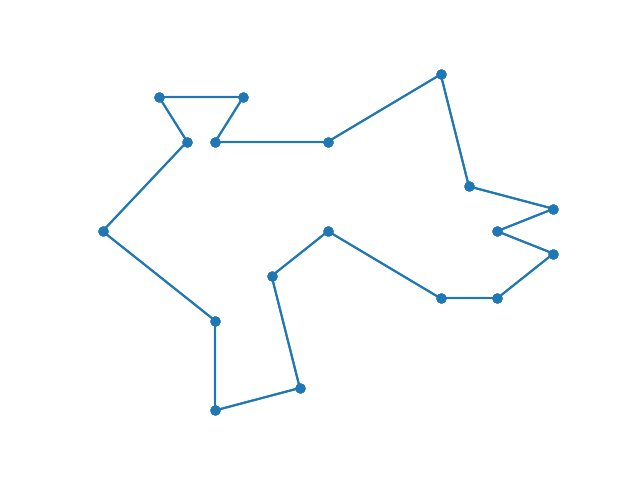
\includegraphics[width = 0.5\textwidth]{experiments/random.png}
    \caption{Arbitrarily shaped polygon.}
    \label{fig:random}
\end{figure}

We will compare how the guards move when we are using all the heuristics to when we are not using momentum. They will start at the same fixed position in both cases.

Figure \ref{fig:no_momentum} displays the area seen per iteration for the arbitrary polygon Both the total area seen and the individual area seen by each are shown. Starting with almost the whole area seen, the guards are eventually optimally placed in a position from which the whole polygon is seen. Nonetheless, using momentum clearly makes a difference in Subfigure \ref{fig:no_momentum1}, than when not using it in Subfigure \ref{fig:no_momentum2}. Using momentum allows the overall seen area to keep a steady trajectory towards its maximum. Additionally, guards quickly find their optimum in only 4 iterations, without many oscillations. In Subfigure \ref{fig:no_momentum2} however we can observe how the total area fluctuates. The guards also display large jumps close to iterations 5 and 20. These jumps cause the overall progress towards the optimum to be less stable. For example, when guard 2 has a sudden drop in the area it sees around iteration 5, the total area seen naturally drops as well, and only recovers after iteration 20, when guard 0 makes another large jump. This behaviour also suggests that the movement of one guard can heavily influence others, resulting in a noisy behaviour and in a higher number of iterations.
% Subfigure \ref{fig:no_momentum1} displays a more smoothened out trajectory for each guard. 
Therefore, it becomes clearer how momentum allows the smoothening of noisy guard movements. Additionally, we reckon that because guards are holding a steadier trajectory, they are more likely to achieve the optimum in less iterations (in this example, 3). When not using momentum, the number of iterations increases substantially to 24. Momentum thus is a crucial improving heuristic to our whole algorithm, both in speedup and in the smoothness of the process.

\begin{figure}[h!]
    \centering
    \begin{subfigure}{0.45\textwidth}
        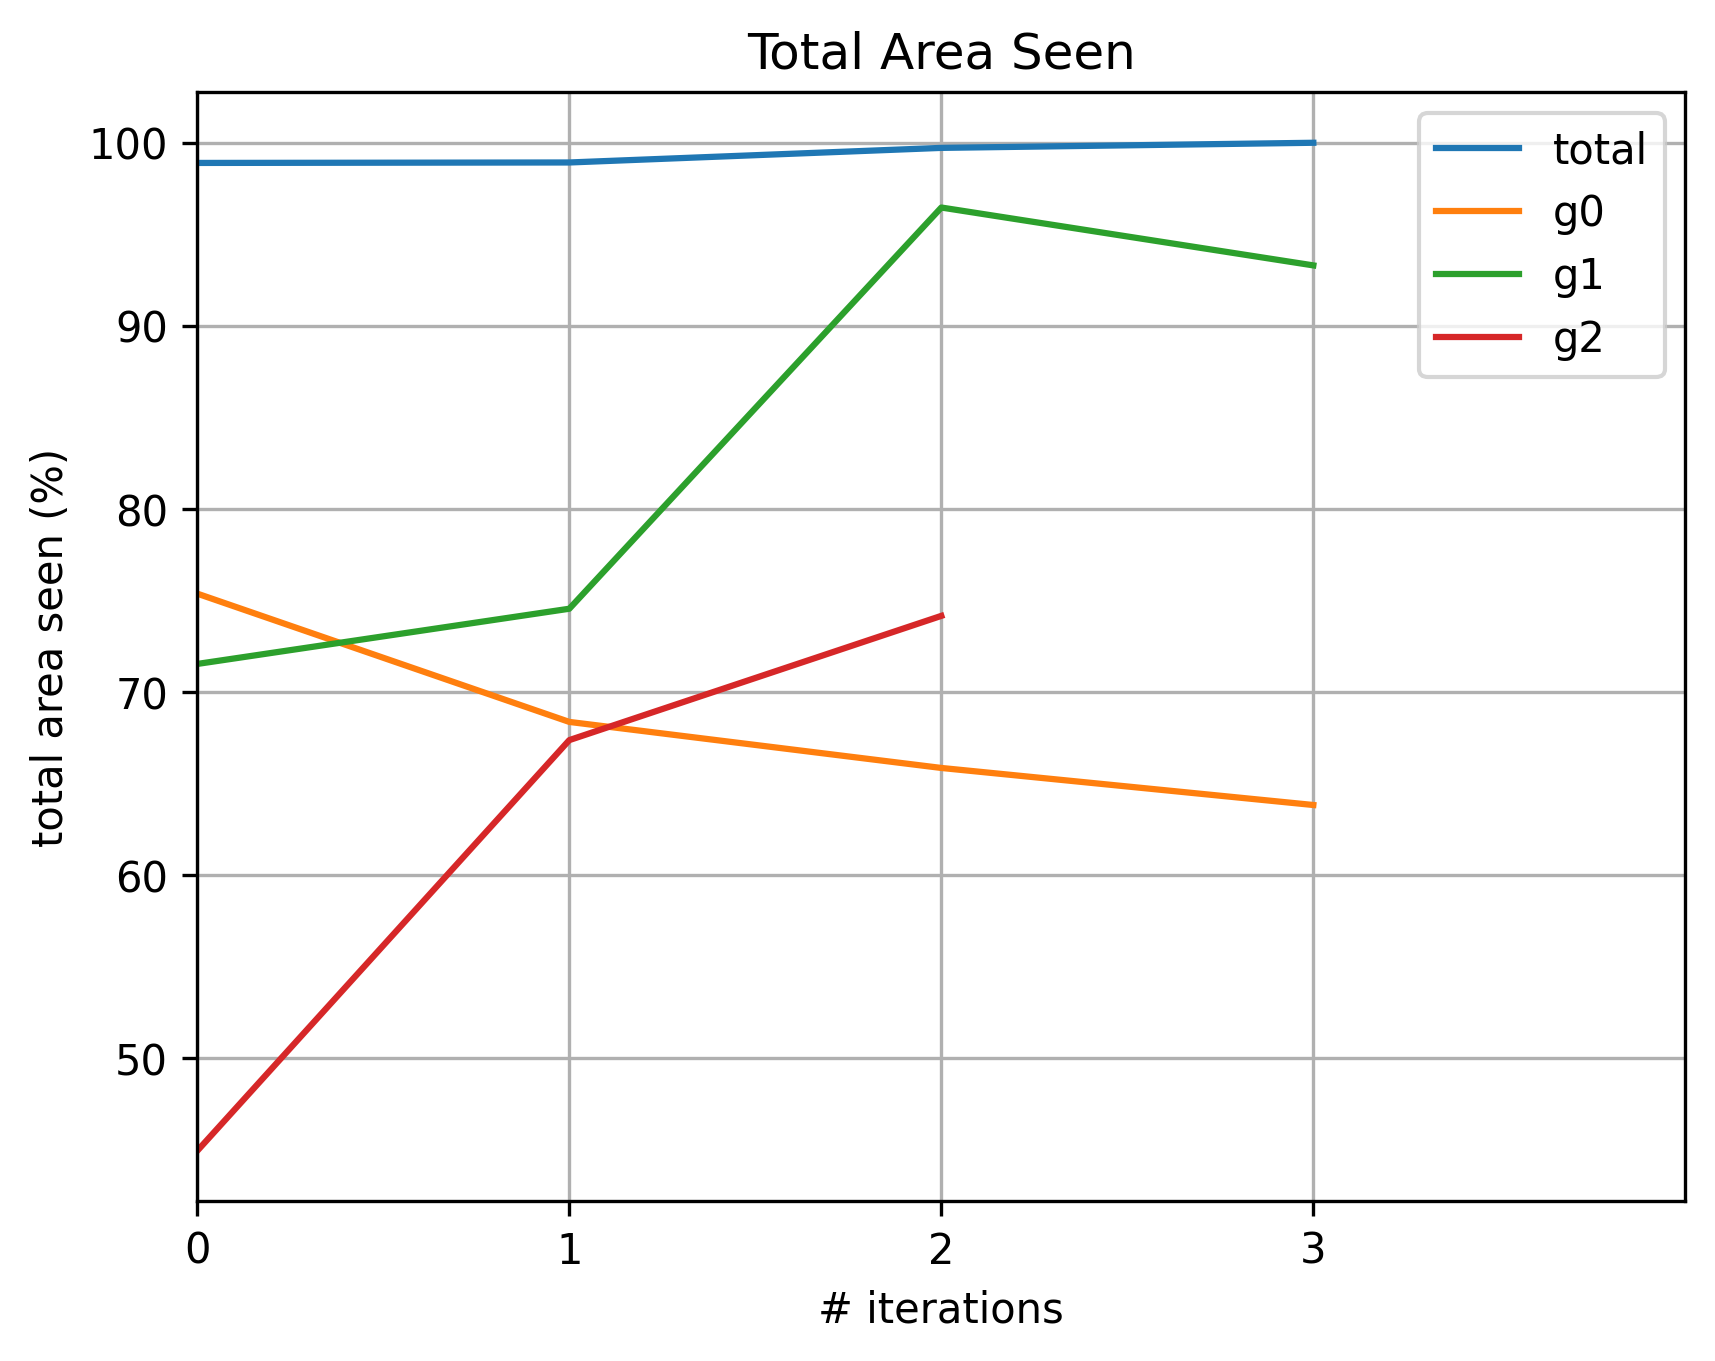
\includegraphics[width = \textwidth]{experiments/area_random_all.png}
        \caption{All heuristics.}
        \label{fig:no_momentum1}
    \end{subfigure}
    \begin{subfigure}{0.45\textwidth}
        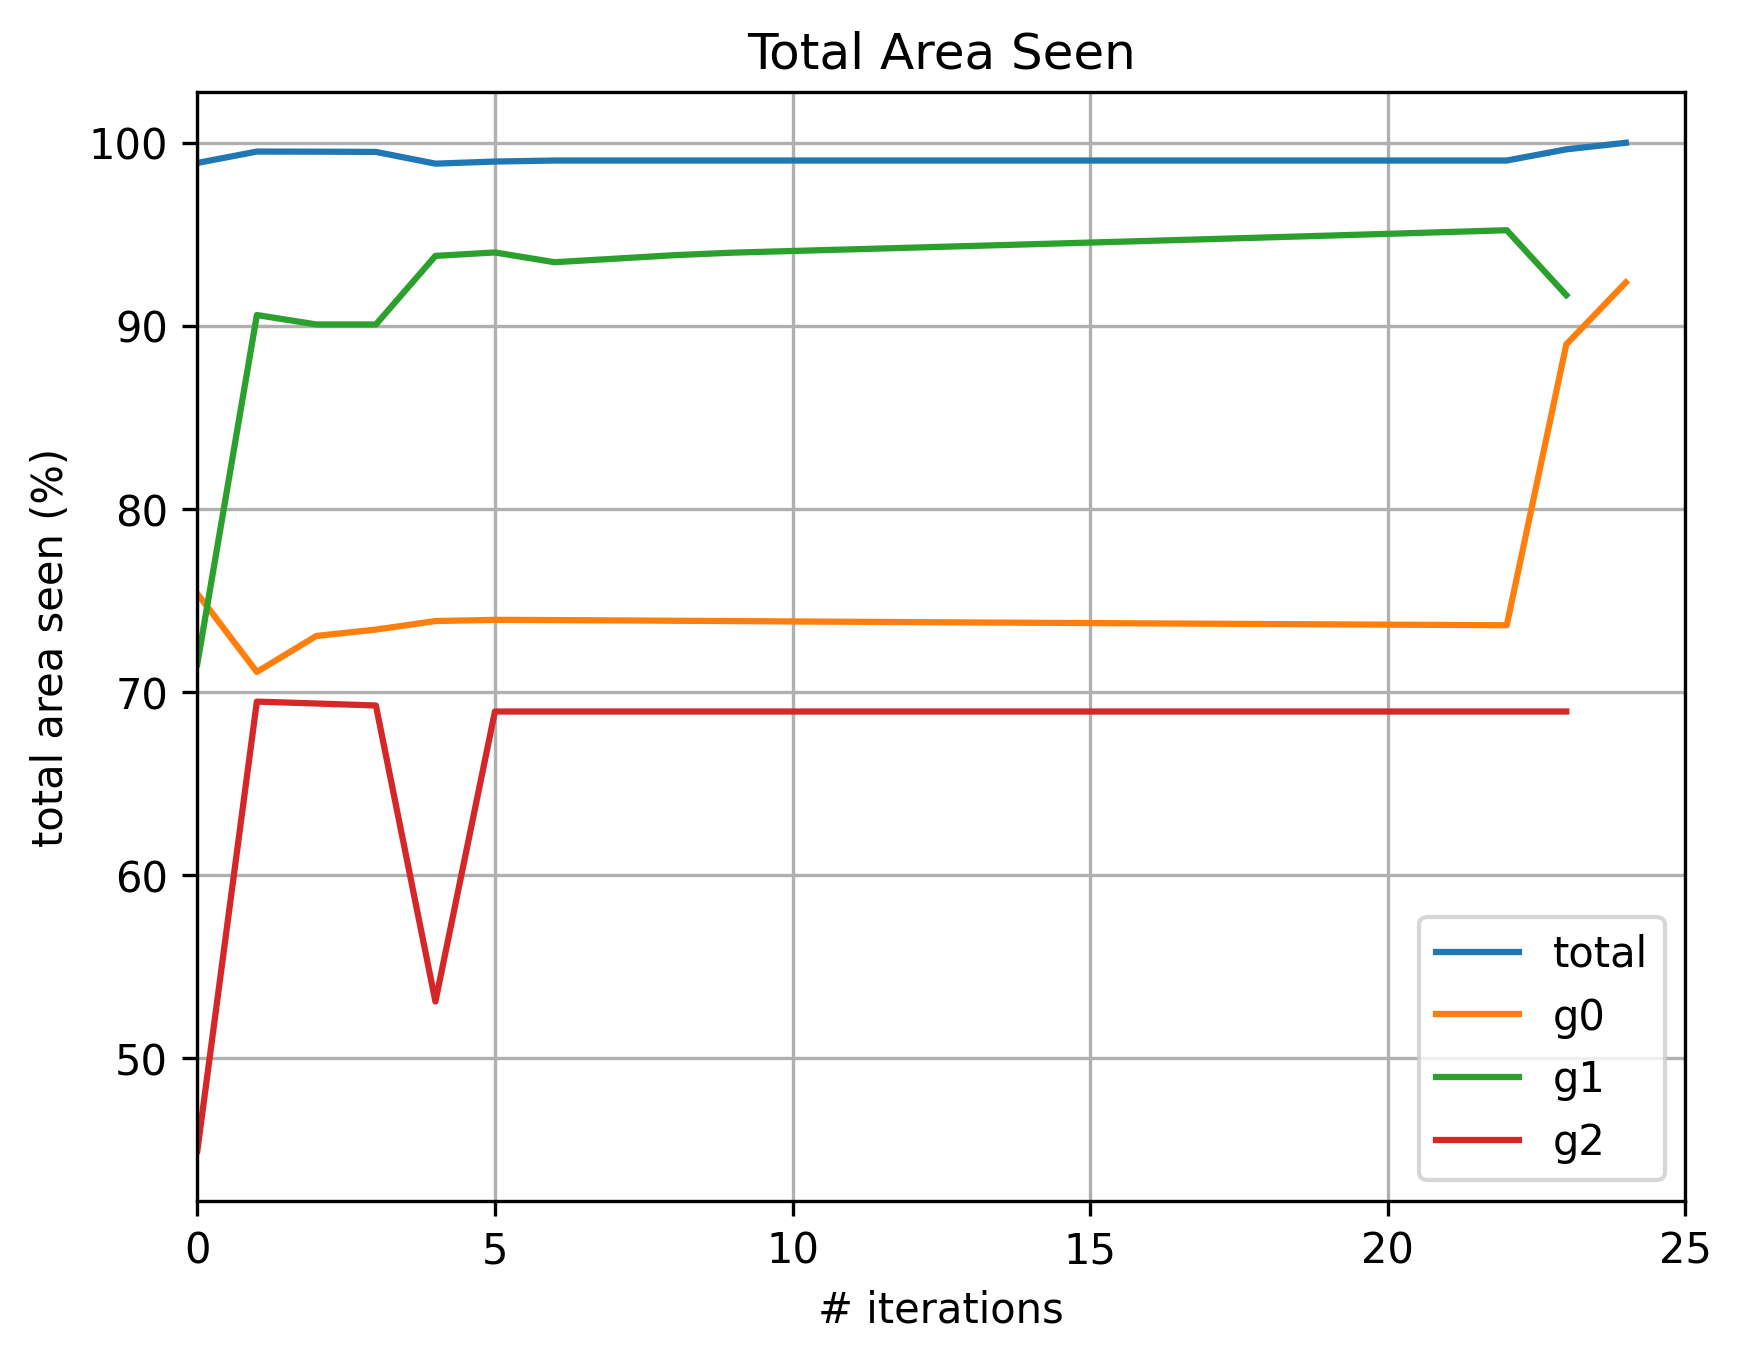
\includegraphics[width = \textwidth]{experiments/area_random_no_momentum.png}
        \caption{No momentum.}
        \label{fig:no_momentum2}
    \end{subfigure}
    \caption{Total area seen per iteration for an arbitrary polygon guarded by 3 guards.}
    \label{fig:no_momentum}
\end{figure}

\subsubsection{Without Line Search}
In this section we will discuss the impact line search has on the overall behaviour of the algorithm. As introduced in Section \ref{sec:line_search}, line search determines how far a guard should move into the optimal direction. In this way, it computes the optimal position of a guard on the direction line given a step size.

For our experiments, we will be using a step size factor of 2. This will allow us to search a larger space of position possibilities knowing the direction of the gradient descent. 
Namely, we will start with a factor of $\frac 1 x$, and we will increase it by a factor of $s$ up to factor $x$. We choose step size factor $s = 2$ and $x = 32$ so that we are able to choose in between 10 positions at every iteration. We will pick for the best solution along all the step size based on the largest area increase. Firstly, we will start with a more finely-grated search closer to the actual value of the gradient. This step will check whether the gradient descent overshoots. Then, we will check farther away from the actual value of the gradient for the case that a larger gain in the guard positioning is possible.

A suggestive way to observe how well Line Search works is with the comb polygon with four teeth from Figure \ref{fig:comb}.

\begin{figure}[h!]
    \centering
    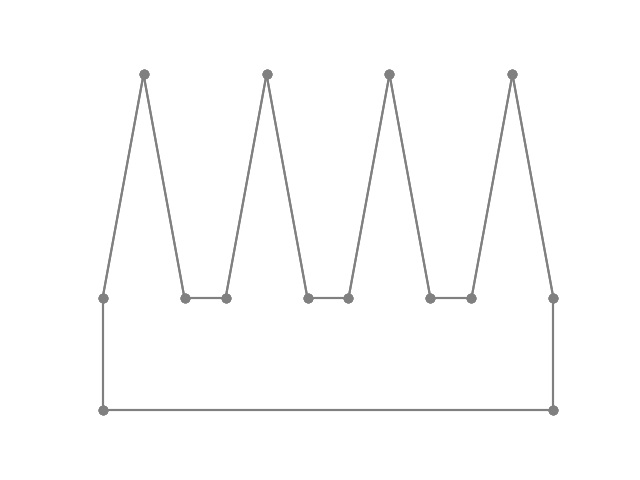
\includegraphics[width = 0.5\textwidth]{experiments/comb.png}
    \caption{Polygon in the shape of a comb with four teeth.}
    \label{fig:comb}
\end{figure}

We will compare how the guards move when we are using all the heuristics to when we are not using line search. They will start at the same fixed position in both cases.

Figure \ref{fig:no_line_search} displays the area seen per iteration for the comb polygon with four teeth. Both the total area seen and the individual area seen by each guard are shown. Starting with around 82.5\% total area seen, the guards are eventually optimally placed in a position from which the whole polygon is seen. Nonetheless, using line search clearly makes a difference between Subfigures \ref{fig:no_line_search1} and \ref{fig:no_line_search2}. The first noticeable difference is the number of iterations. Using line search allows the guards to find their optimal positions in 3 iterations, with a steady increase in the total area seen. On the other hand, not using line search results in the optimal position to be found in more than 80 iterations. What is more, 3 of the guards seem to have found their optimal position after the $30^{\text{th}}$ iteration, whereas the last 50 iterations are spent on only one guard finding its own.

Therefore, we reckon that line search significantly and more efficiently speeds up the process of finding the optimal position for each guard. In this way, each guard moves faster to its optimal position and avoids creating situations where multiple guards that have found their optimal position have to wait for only one guard to find its own.


\begin{figure}[h!]
    \centering
    \begin{subfigure}{0.45\textwidth}
        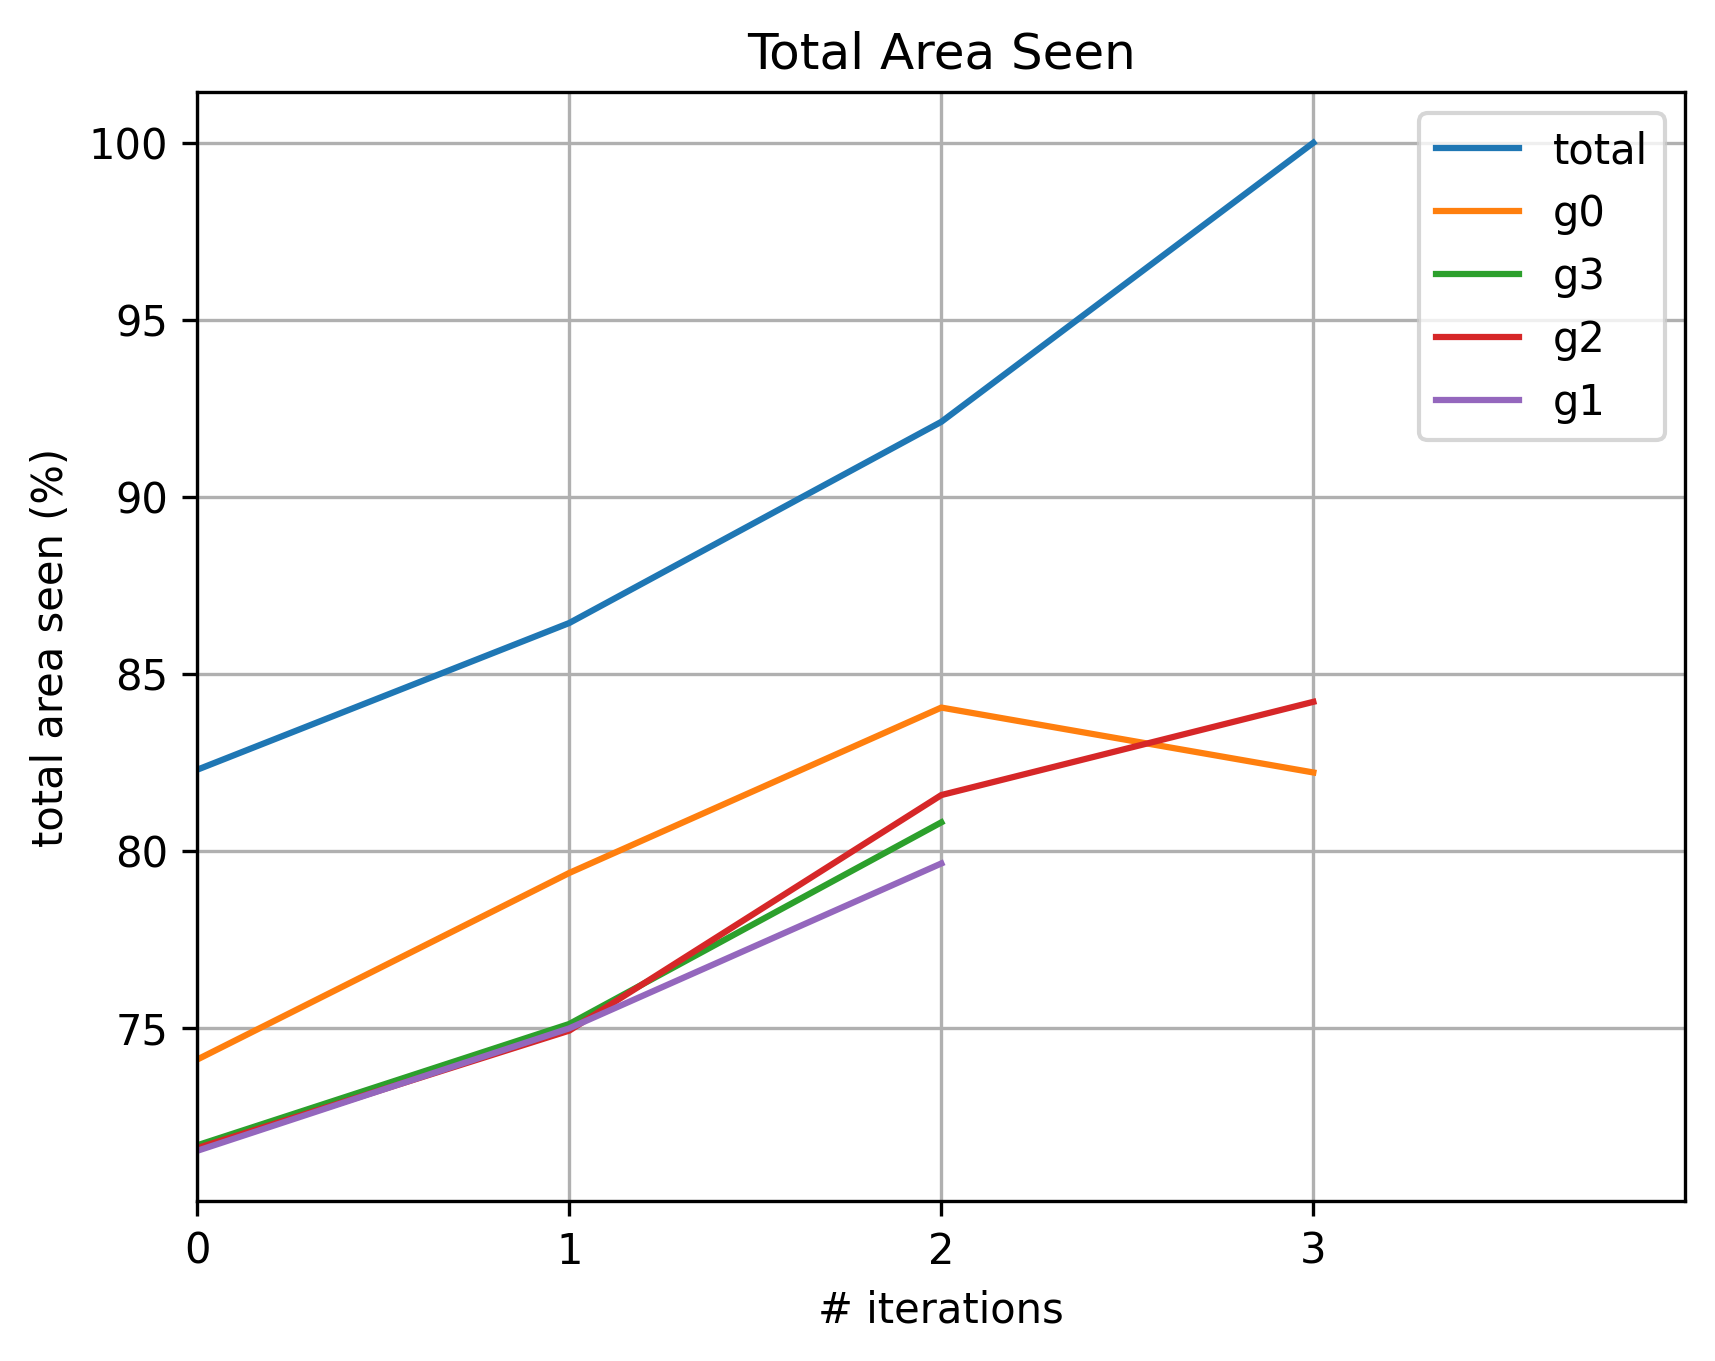
\includegraphics[width = \textwidth]{experiments/area_comb_easy_all.png}
        \caption{All heuristics.}
        \label{fig:no_line_search1}
    \end{subfigure}
    \begin{subfigure}{0.45\textwidth}
        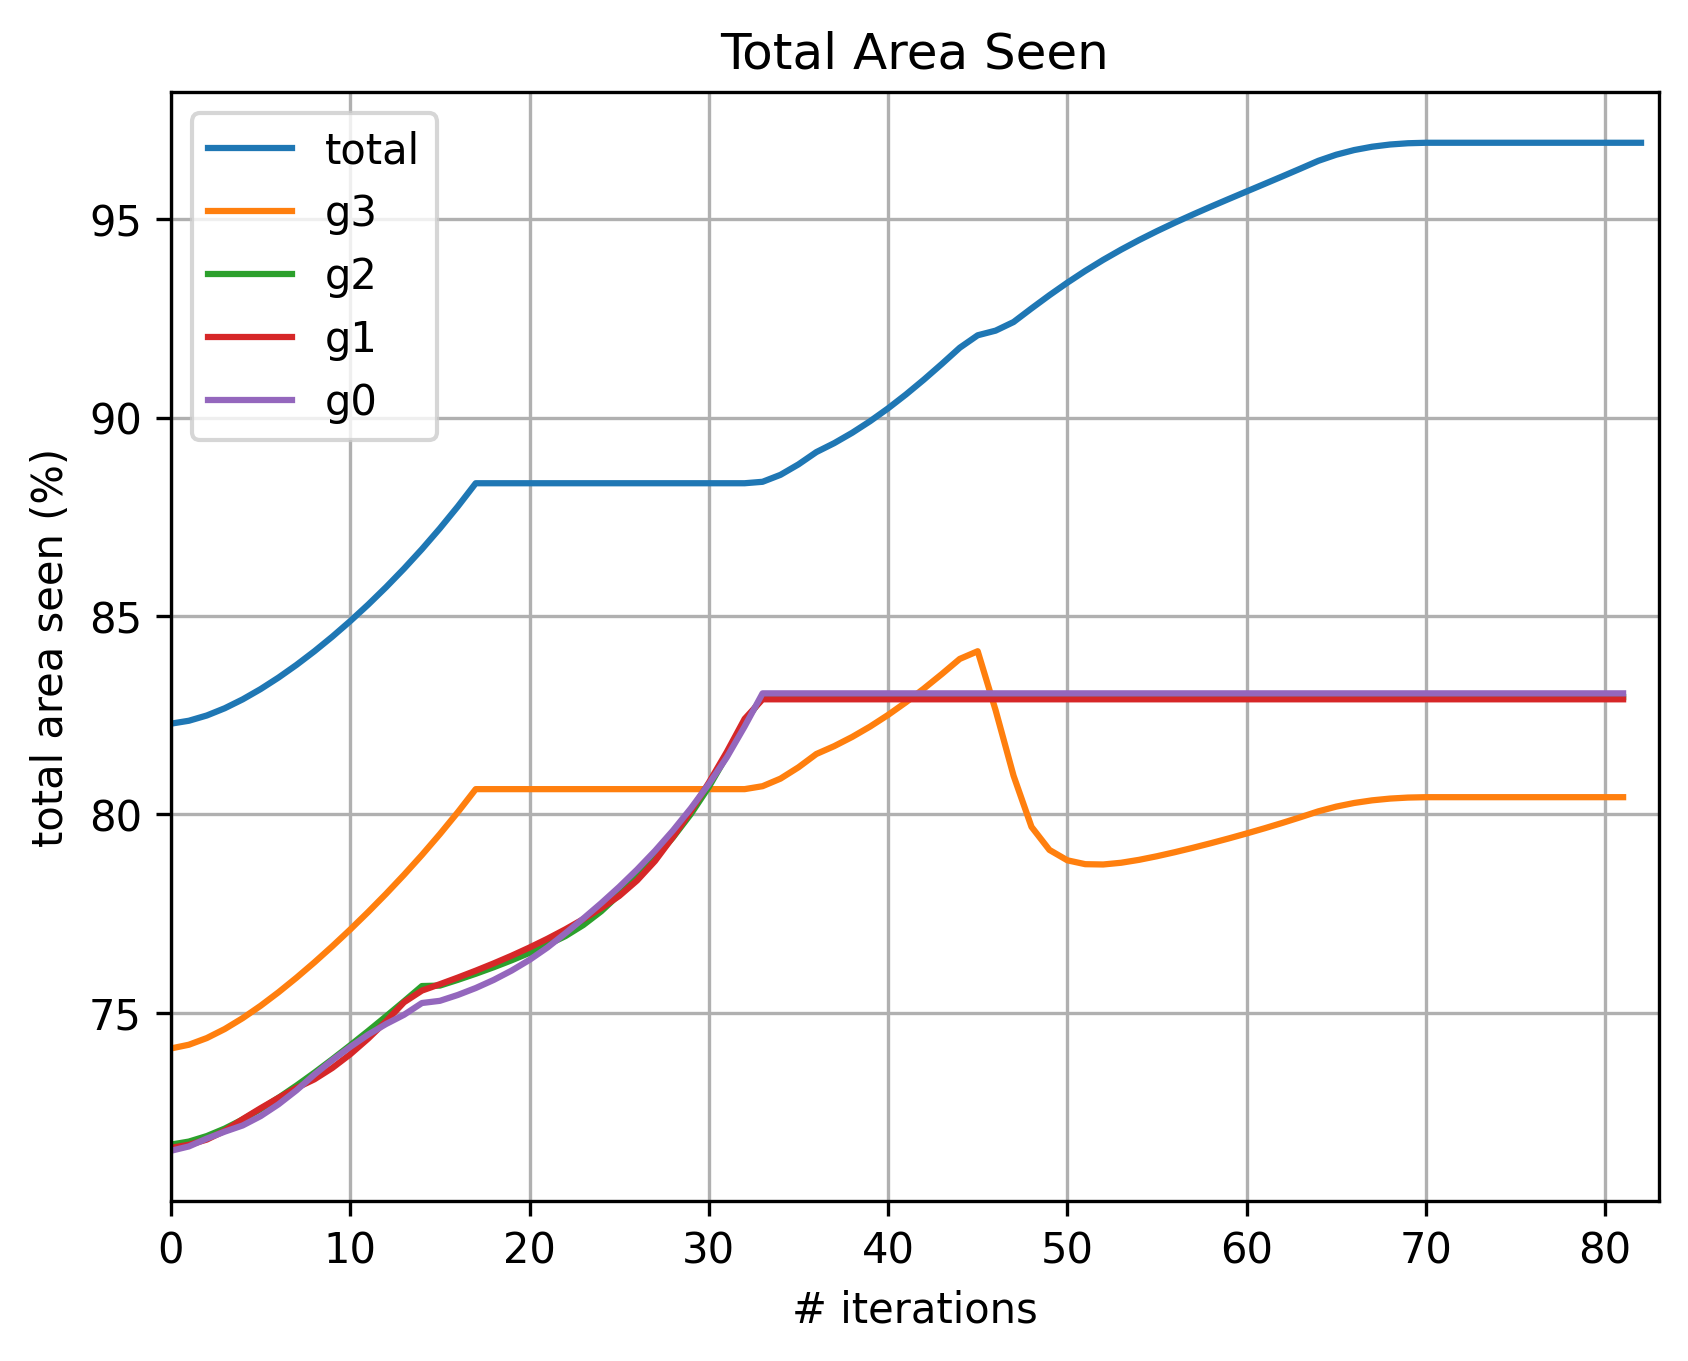
\includegraphics[width = \textwidth]{experiments/area_comb_no_linear_search.png}
        \caption{No line search.}
        \label{fig:no_line_search2}
    \end{subfigure}
    \caption{Total area seen per iteration for the comb polygon with four teeth.}
    \label{fig:no_line_search}
\end{figure}

\subsubsection{Without Pulling Onto Reflex Vertex}
In this section we will discuss the impact the pull onto the reflex vertex heuristic has on the behaviour of the algorithm. Section \ref{sec:pull_onto} introduced the pulling guards on top of a reflex vertex heuristic. This heuristic tackles the idea that if a guard is ``close enough'' to a reflex vertex, then the locally maximum seen area would be achieved by placing the guard on top of the reflex vertex. We have defined a guard being ``close enough'' to a reflex vertex as closer than two thirds of the minimum distance between any two reflex vertices in the polygon.

We will compare how the guards move when we are using all the heuristics to when we are not pulling them onto reflex vertices. The guards will start at the same fixed position in both cases.

Figure \ref{fig:no_pull} displays the two reflex vertex pull cases: Subfigures \ref{fig:all_pull_pos0} and \ref{fig:all_pull_pos1} show how the green guard movement changes when it is placed onto the reflex vertex; Subfigures \ref{fig:no_pull_pos0} and \ref{fig:no_pull_pos1} show how the guard movement changes when the guard is pulled towards the reflex vertex, but not pulled onto it. We can observe how in Subfigure \ref{fig:all_pull_pos1} the green guard is placed onto the reflex vertex. It then strives to reach the unseen polygon part in the upper left corner. On the other hand, in Subfigure \ref{fig:no_pull_pos1} the guard moved away from the reflex vertex. 
% However, its movement still indicates that it should move back, closer to the reflex vertex it was not placed on. 
These events can also be observed in the two seen area plots in Subfigures \ref{fig:area_all_pull} and Subfigures \ref{fig:area_no_pull}. Clearly, the case when the green guard is not placed on top of the reflex vertex results in more iterations, as seen in Subfigure \ref{fig:area_no_pull}. This is due to the fact that the green guard could not take advantage of the local area maximisation by being placed on the reflex vertex. So, it needs to move around more before finding its optimal path. This is also displayed in how the total area seen lowers and then rises in between iterations 1 and 4. Conversely, Subfigure \ref{fig:area_all_pull} displays how the green guard has quickly moved towards the last part of the polygon that was not yet seen. This resulted in a steady increase in the total seen area.

Therefore, we believe that pulling guards on top of reflex vertices when they are ``close enough'' results in the local maximisation of the area seen by those guards. The number of iterations needed to reach the global maximum is thus reduced. So, the efficiency of the algorithm is also positively affected.

\begin{figure}[h!]
    \centering
    \begin{subfigure}{0.45\textwidth}
        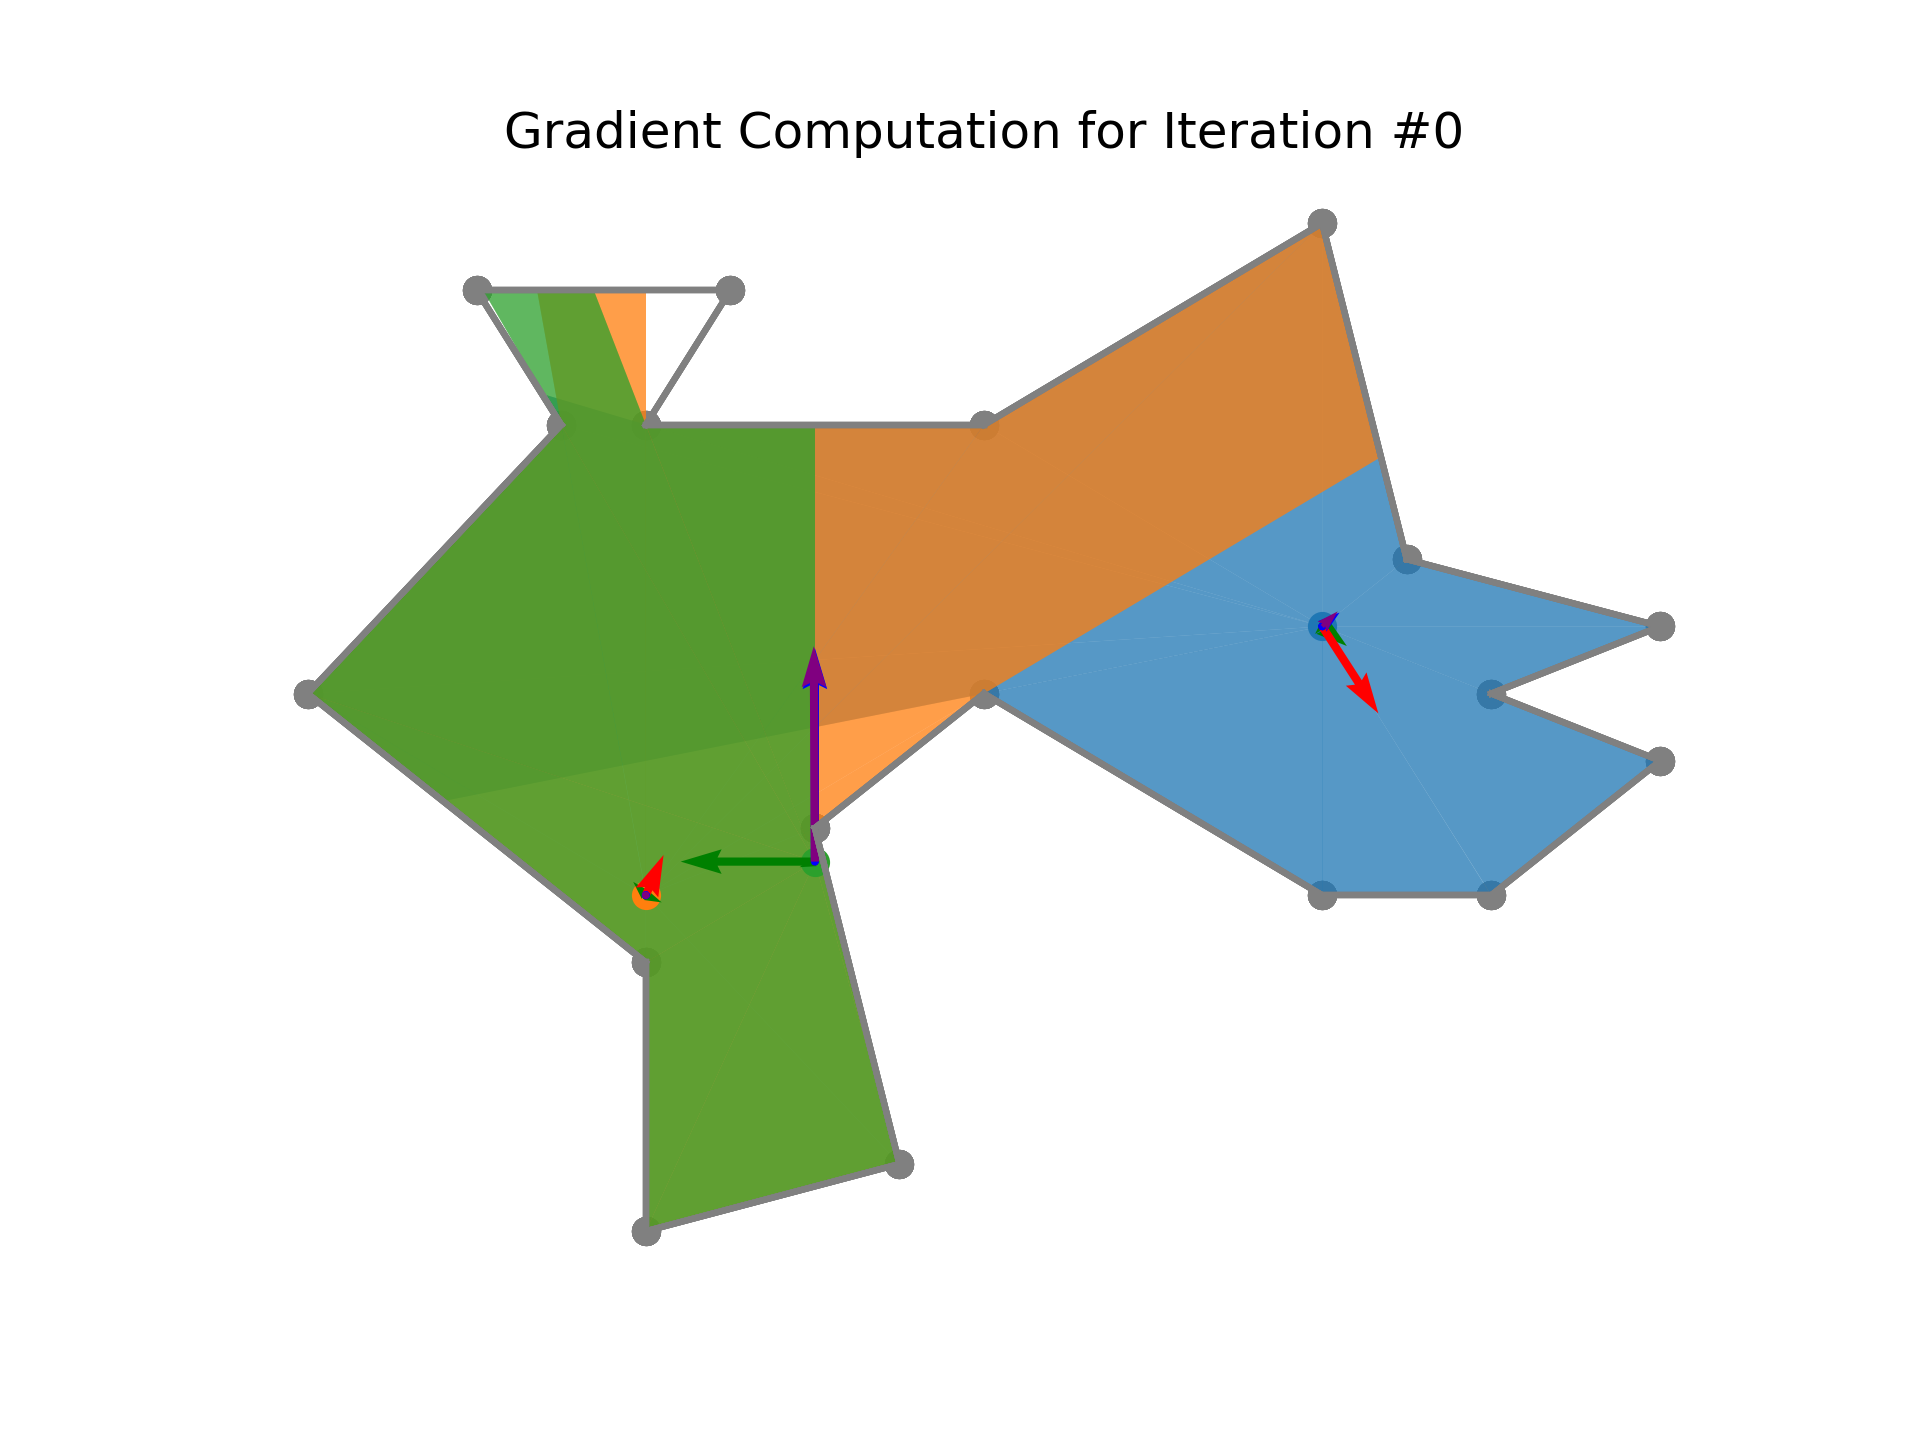
\includegraphics[width = \textwidth]{experiments/random_all_pull_pos0_fixed.png}
        \caption{All heuristics, iteration 0. The green guard is pulled towards the reflex vertex.}
        \label{fig:all_pull_pos0}
    \end{subfigure}
    \hfill
    \begin{subfigure}{0.45\textwidth}
        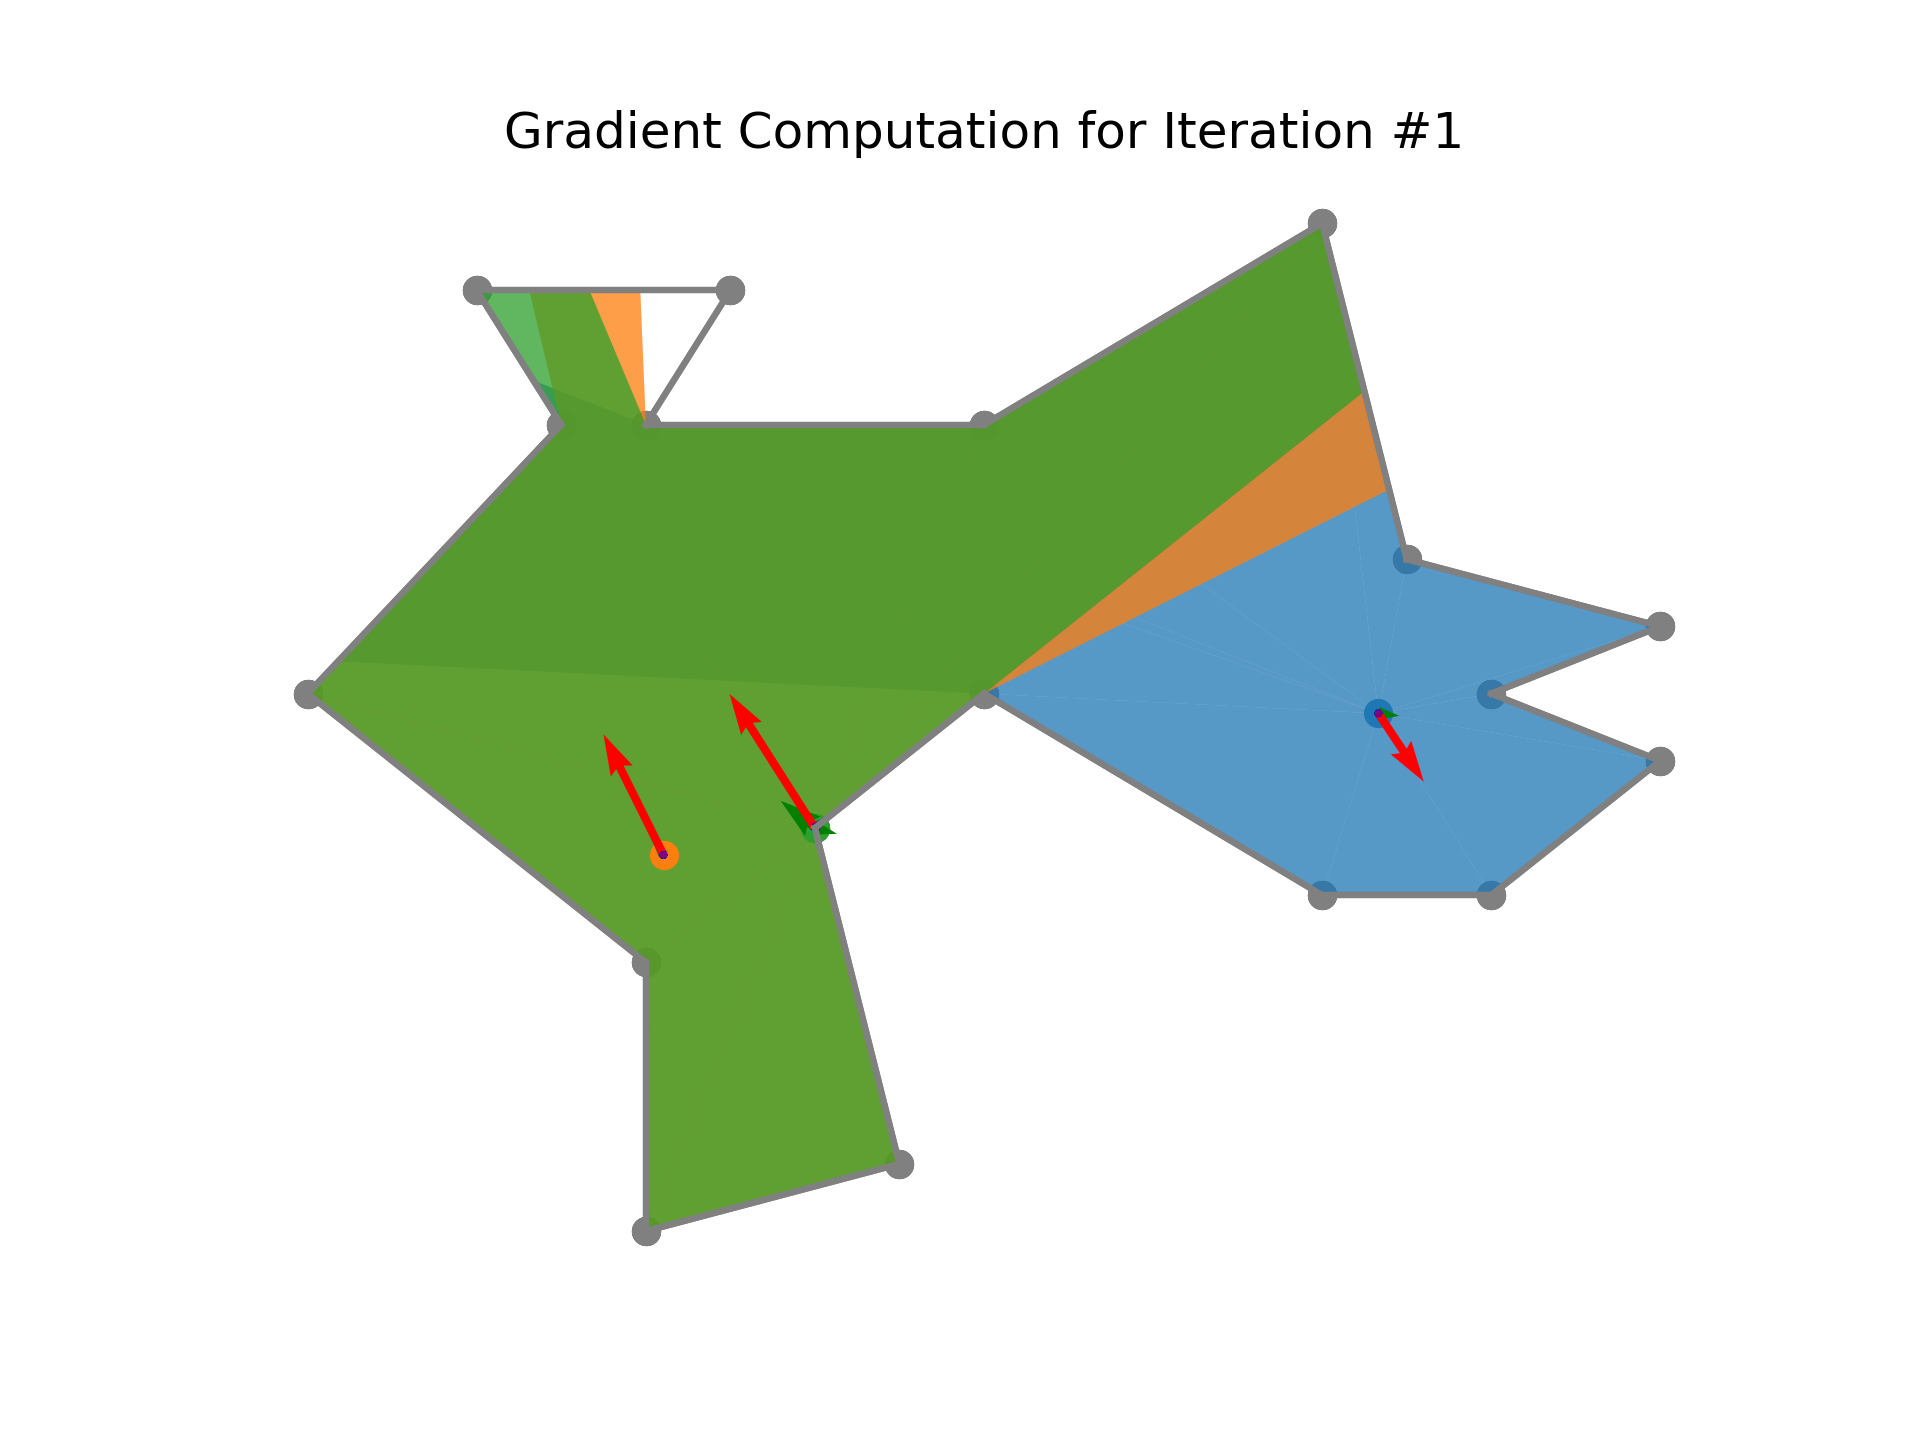
\includegraphics[width = \textwidth]{experiments/random_all_pull_pos1_fixed.png}
        \caption{All heuristics, iteration 1. The green guard is onto the reflex vertex.}
        \label{fig:all_pull_pos1}
    \end{subfigure}
    \vfill
    \begin{subfigure}{0.45\textwidth}
        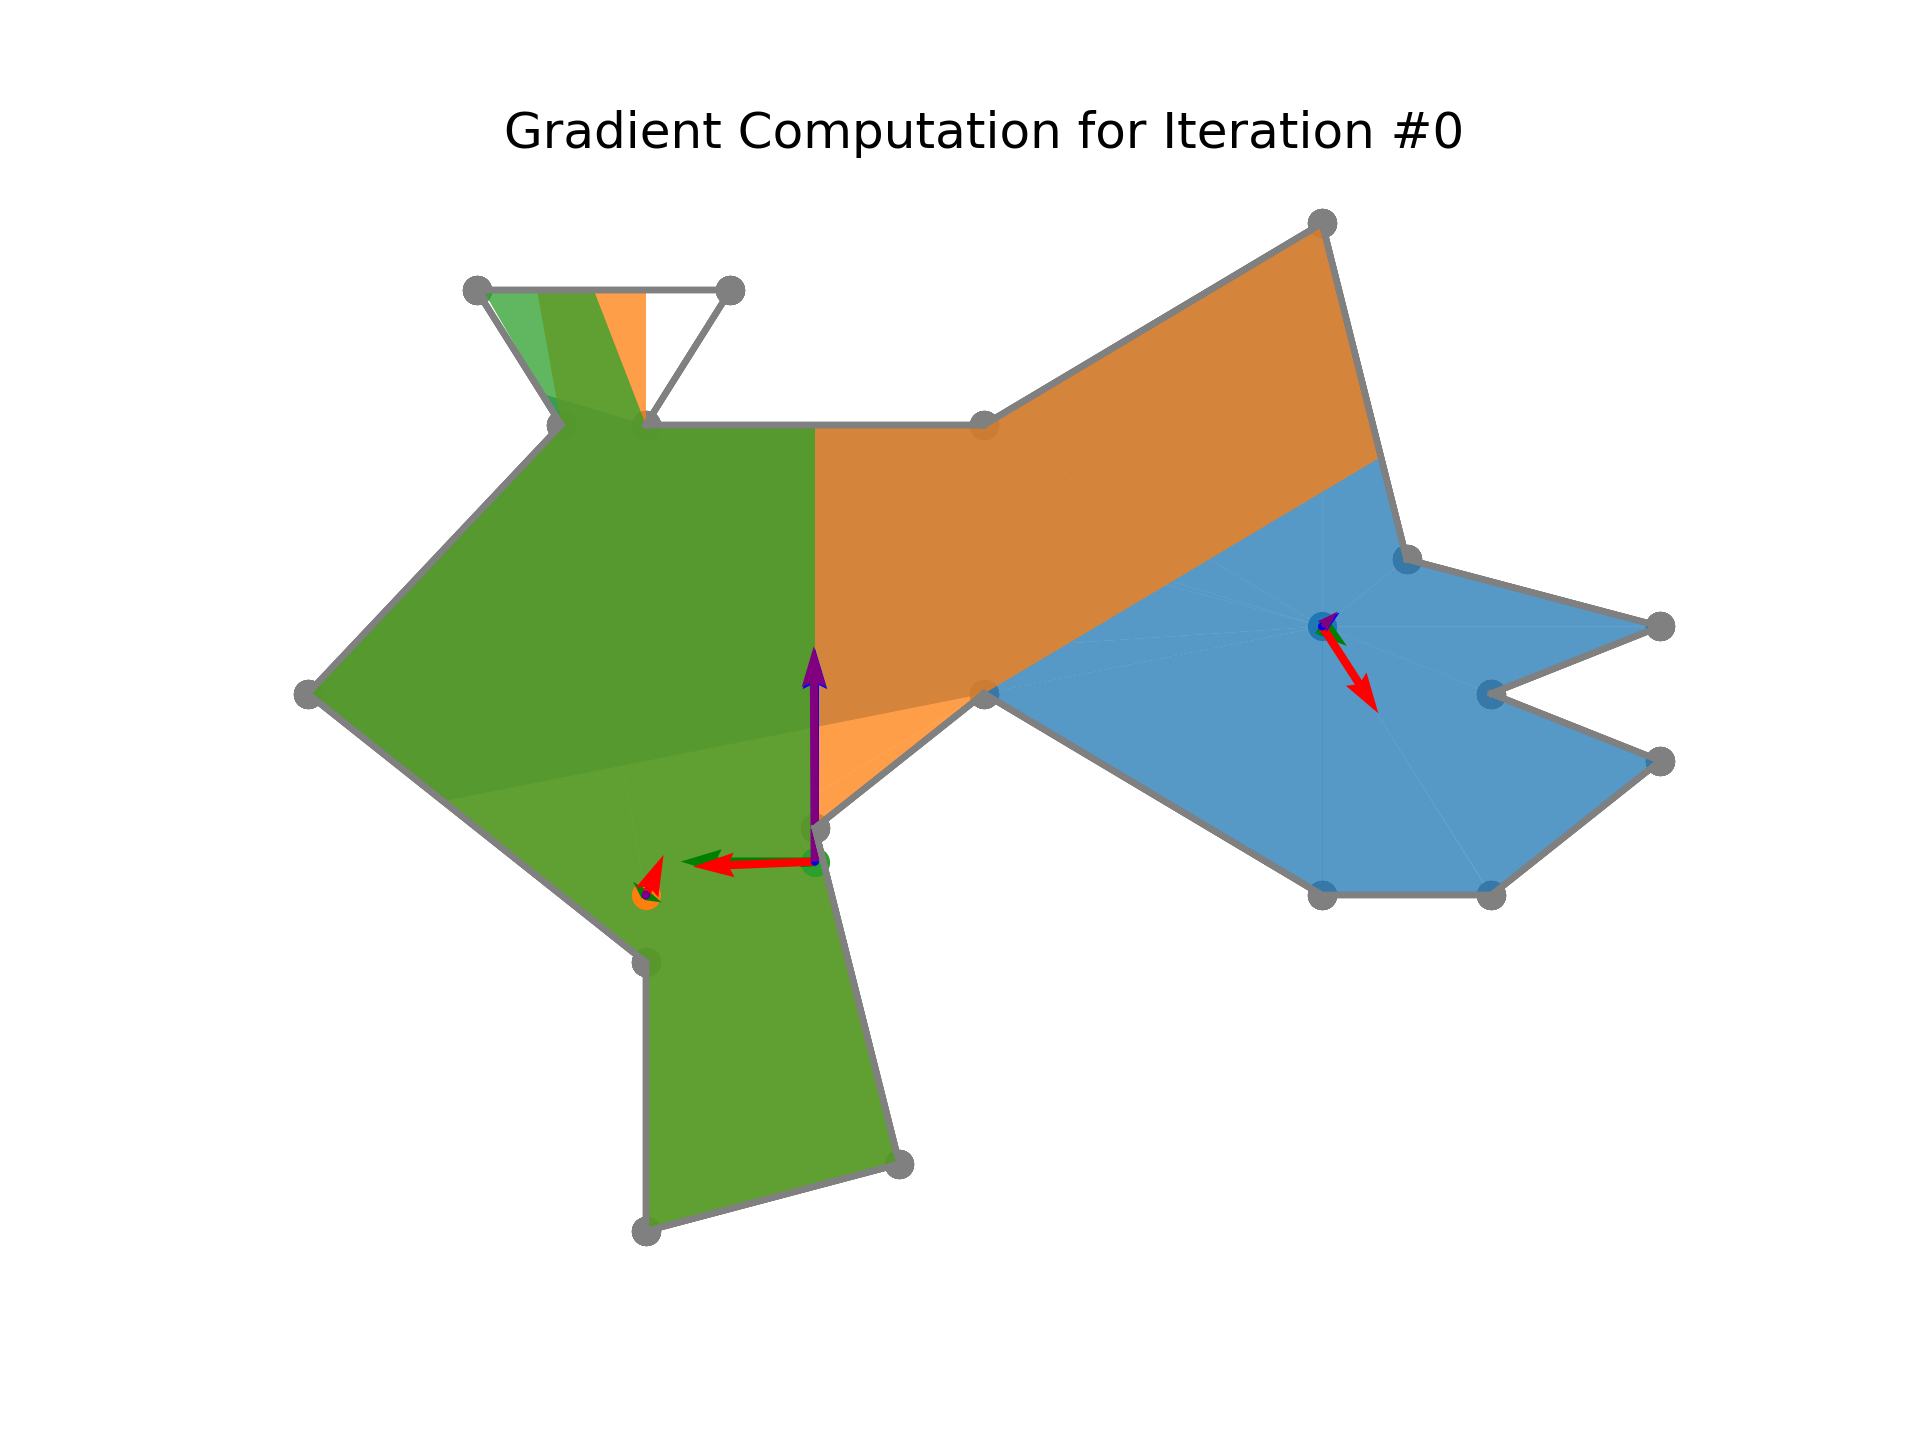
\includegraphics[width = \textwidth]{experiments/random_no_pull_pos0_fixed.png}
        \caption{No pull onto the reflex vertex, iteration 0. The green guard is pulled towards the reflex vertex.}
        \label{fig:no_pull_pos0}
    \end{subfigure}
    \hfill
    \begin{subfigure}{0.45\textwidth}
        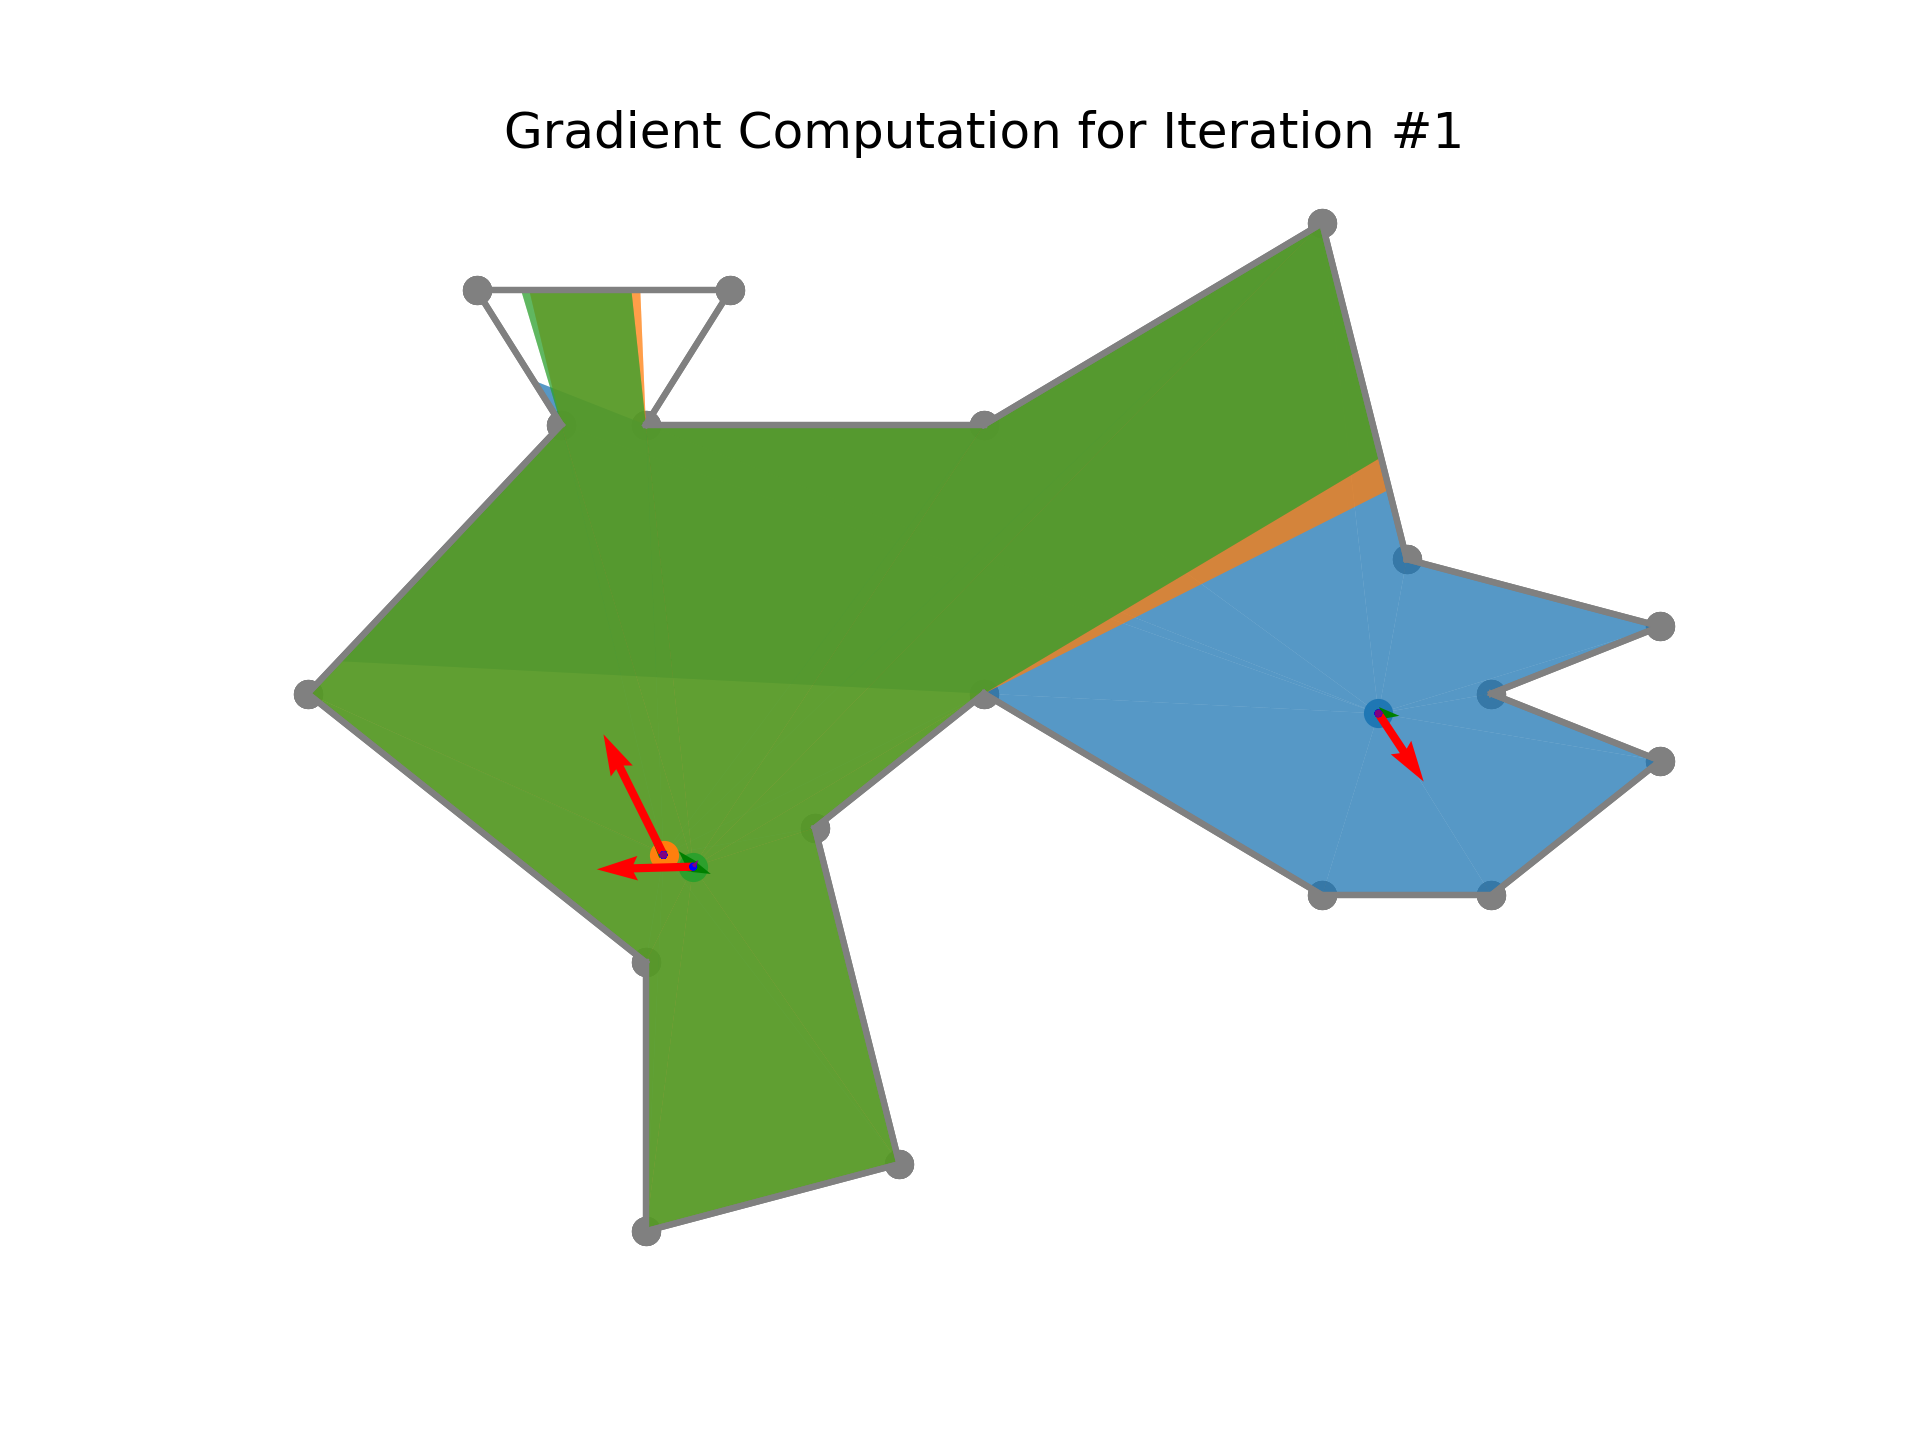
\includegraphics[width = \textwidth]{experiments/random_no_pull_pos1_fixed.png}
        \caption{No pull onto the reflex vertex, iteration 1. The green guard is placed according to the momentum computation.}
        \label{fig:no_pull_pos1}
    \end{subfigure}
    \vfill
    \begin{subfigure}{0.45\textwidth}
        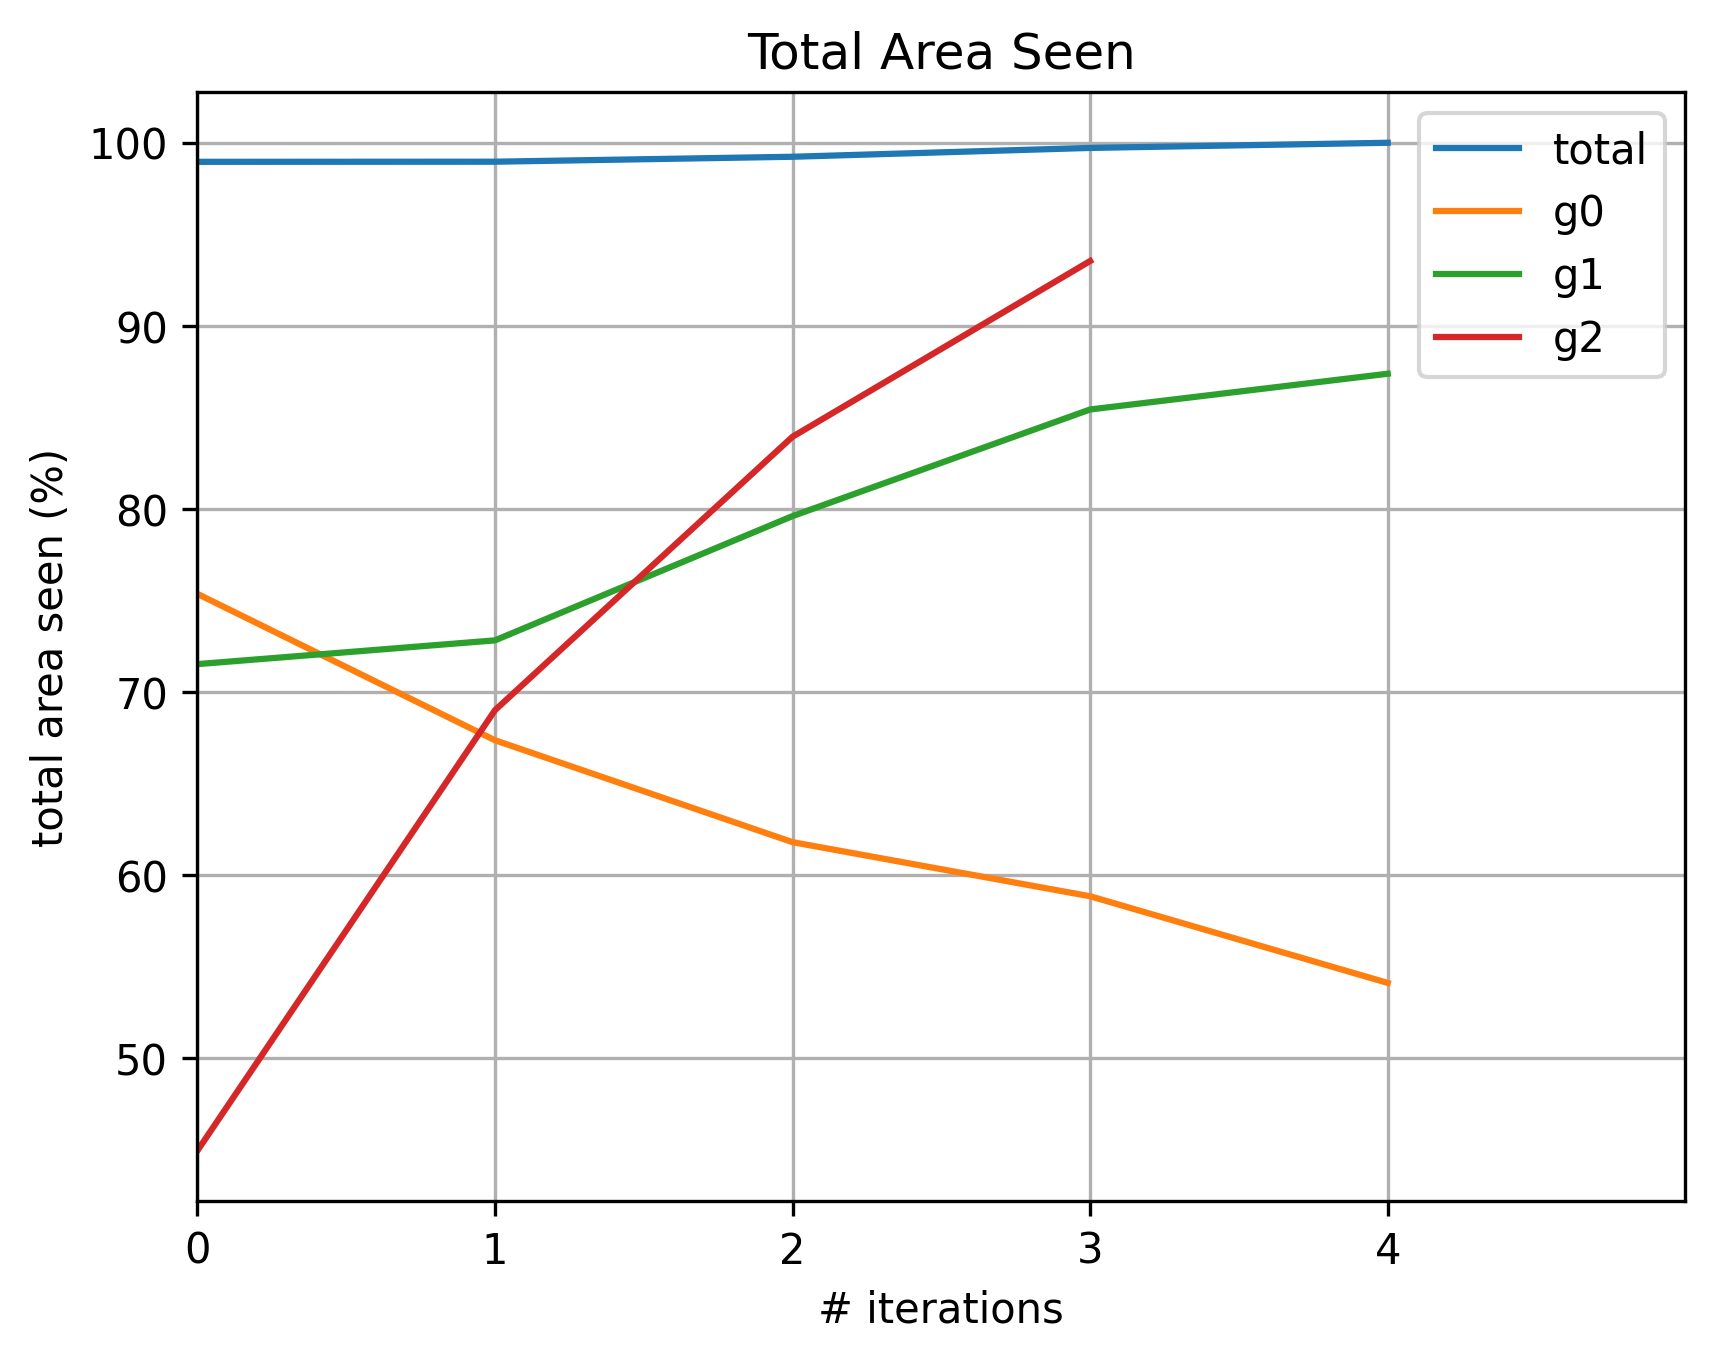
\includegraphics[width = \textwidth]{experiments/area_random_all_fixed.png}
        \caption{Seen area for all heuristics.}
        \label{fig:area_all_pull}
    \end{subfigure}
    \hfill
    \begin{subfigure}{0.45\textwidth}
        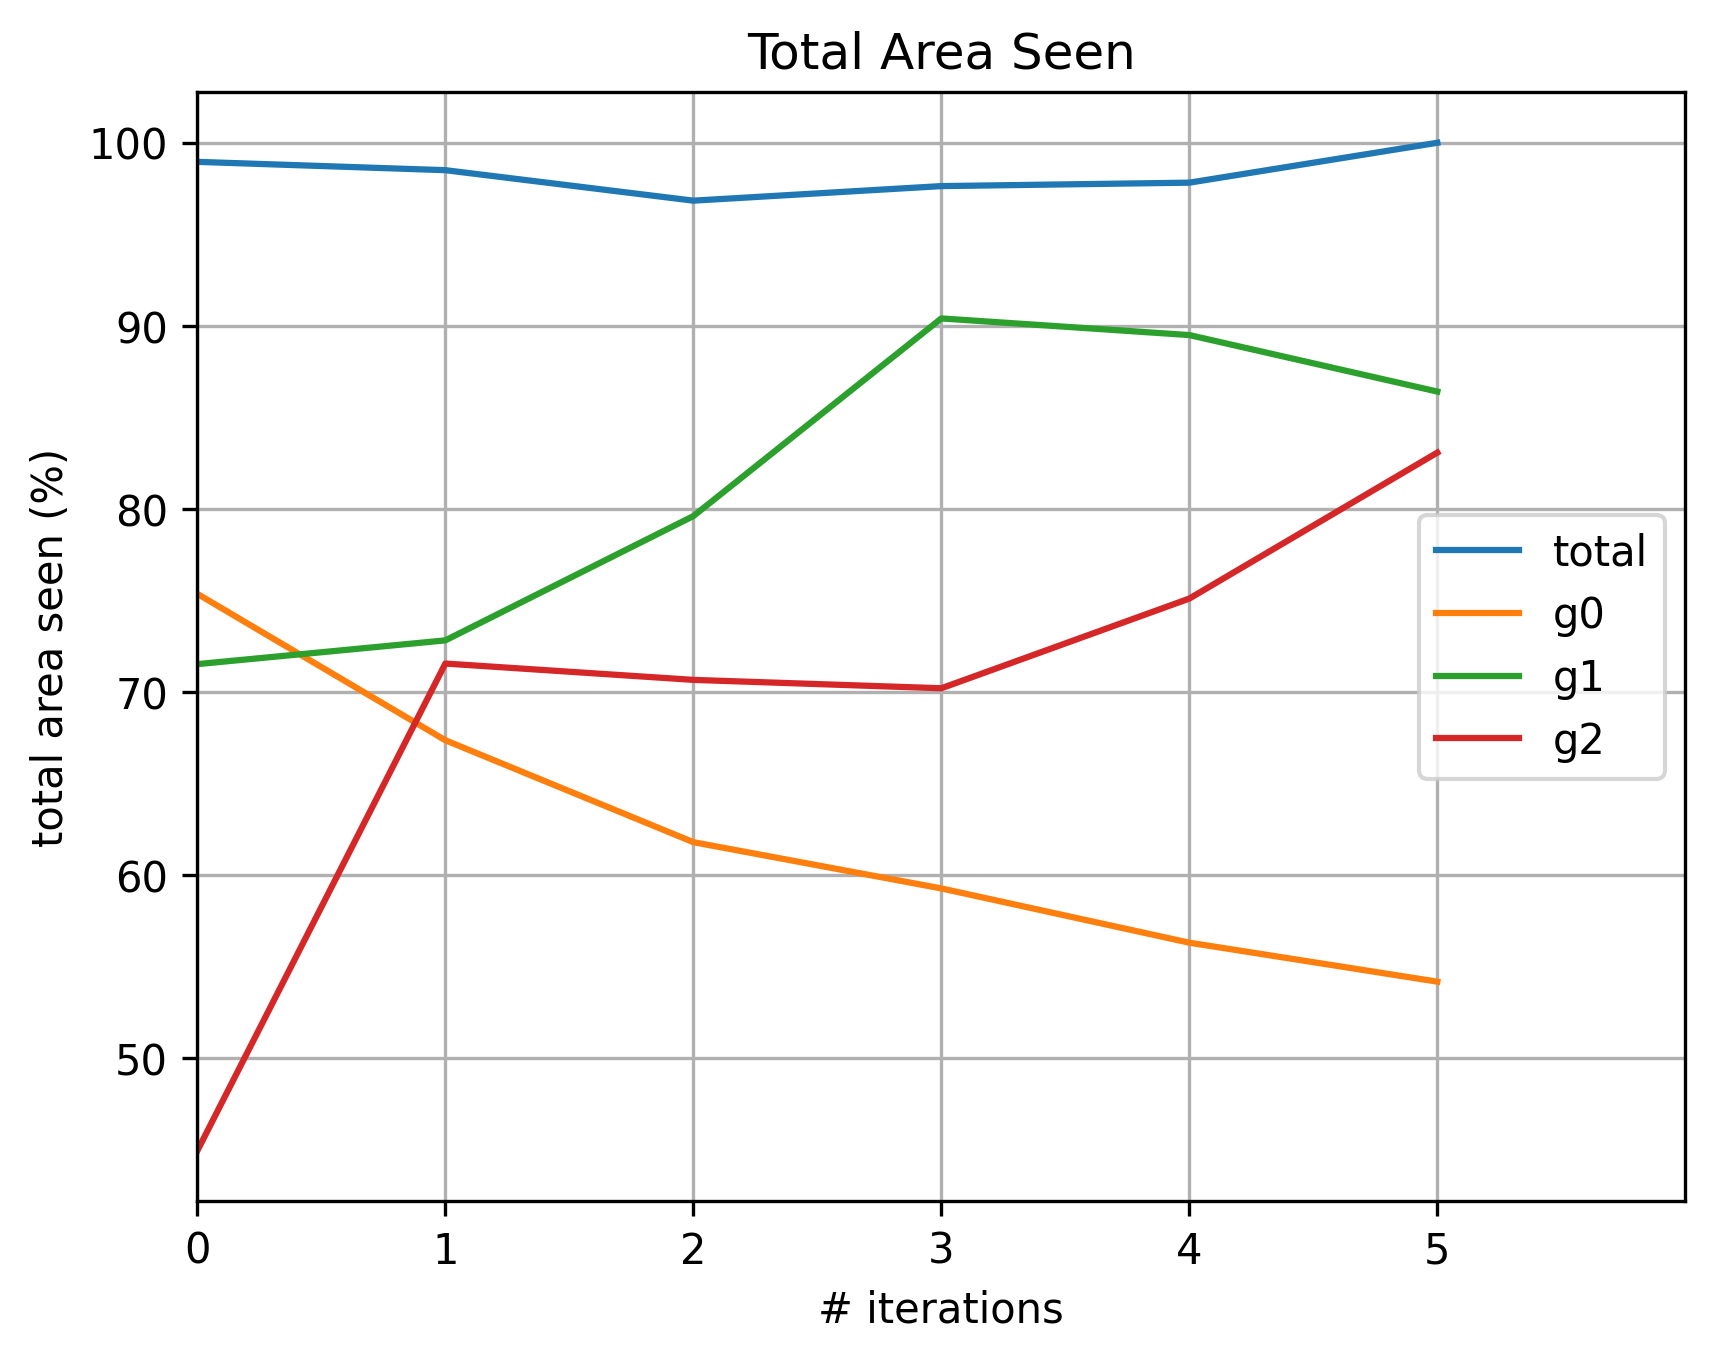
\includegraphics[width = \textwidth]{experiments/area_random_no_pull_fixed.png}
        \caption{Seen area without pull onto reflex vertices.}
        \label{fig:area_no_pull}
    \end{subfigure}
    \caption{Comparison between a guard being and not being pulled onto a reflex vertex in an arbitrary polygon.}
    \label{fig:no_pull}
\end{figure}

\subsubsection{Without Pull Capping}
In this section we will discuss how not capping the pull towards a reflex vertex influences the overall progression of the guards' movements. Section \ref{sec:pull_capping} introduced the notion of capping the pull towards a reflex vertex. The reason for this choice was to not give the pull the possibility to overpower the value of the momentum. So, if the pull is larger than a factor $\mu$ than the momentum, it is capped at the momentum value of a factor of $\mu$. 

We will compare how the guards move when we are using all the heuristics to when we are not capping the pull towards reflex vertices. We will use the comb polygon with four teeth as example. The guards have a pull cap hyperparameter $\mu = 1$. Thus, if the pull is larger than the momentum, we cap it at the size of the momentum. The reason behind this hyperparameter choice was that it offers a middle ground in between pull capping values that are significantly larger or smaller than the momentum. So, if the pull is as large as the momentum, we will decide to prioritise giving the guard the choice to be pulled onto a reflex vertex if it is ``close enough''.

Figure \ref{fig:no_capping} displays the two reflex vertex pull cases: Subfigures \ref{fig:all_cap_pos0} and \ref{fig:all_cap_pos1} show how the blue guard movement changes when its pull is capped; Subfigures \ref{fig:no_cap_pos0} and \ref{fig:no_cap_pos1} show the opposite. We can observe how in Subfigure \ref{fig:all_cap_pos0} the blue guard has its pull towards the reflex vertex capped. In that case, the pull is not strong enough to move the guard towards the reflex vertex. So, the blue guard moves as its momentum dictates to the position in Subfigure \ref{fig:all_cap_pos1}. This can result in encouraging the guard to explore the polygon more rather than directly moving towards a reflex vertex.
Conversely, Subfigure \ref{fig:no_cap_pos1} displays the blue guard moving closer to the reflex vertex it is pulled to. In subsequent iterations, it is placed on the reflex vertex

Subfigures \ref{fig:area_all_cap} and \ref{fig:area_no_cap} show how the global behaviour of the algorithm is influenced by the capping. Interestingly enough, when capping the pull, the guards' behaviour is more erratic, resulting in more iterations before the whole polygon is seen. On the other hand, using no capping allows a steadier increase in the total area seen. Eventually, the blue guard is drawn and placed onto the reflex vertex. This reinforces the previously discussed idea that placing guards on reflex vertices is beneficial for the overall run of the algorithm. Nonetheless, tuning the hyperparameter $\mu$ is a crucial point of exploration for deciding how and when pull capping would always prove most beneficial.

Therefore, we believe that capping the guards' pull towards a reflex vertex highly depends on the hyperparameter $\mu$ and the shape of the polygon. When not capped, it additionally reinforces the importance of placing guards on reflex vertices. However, when the pull of guards is capped, we are using a more exploratory approach to discovering the polygon.

\begin{figure}[h!]
    \centering
    \begin{subfigure}{0.45\textwidth}
        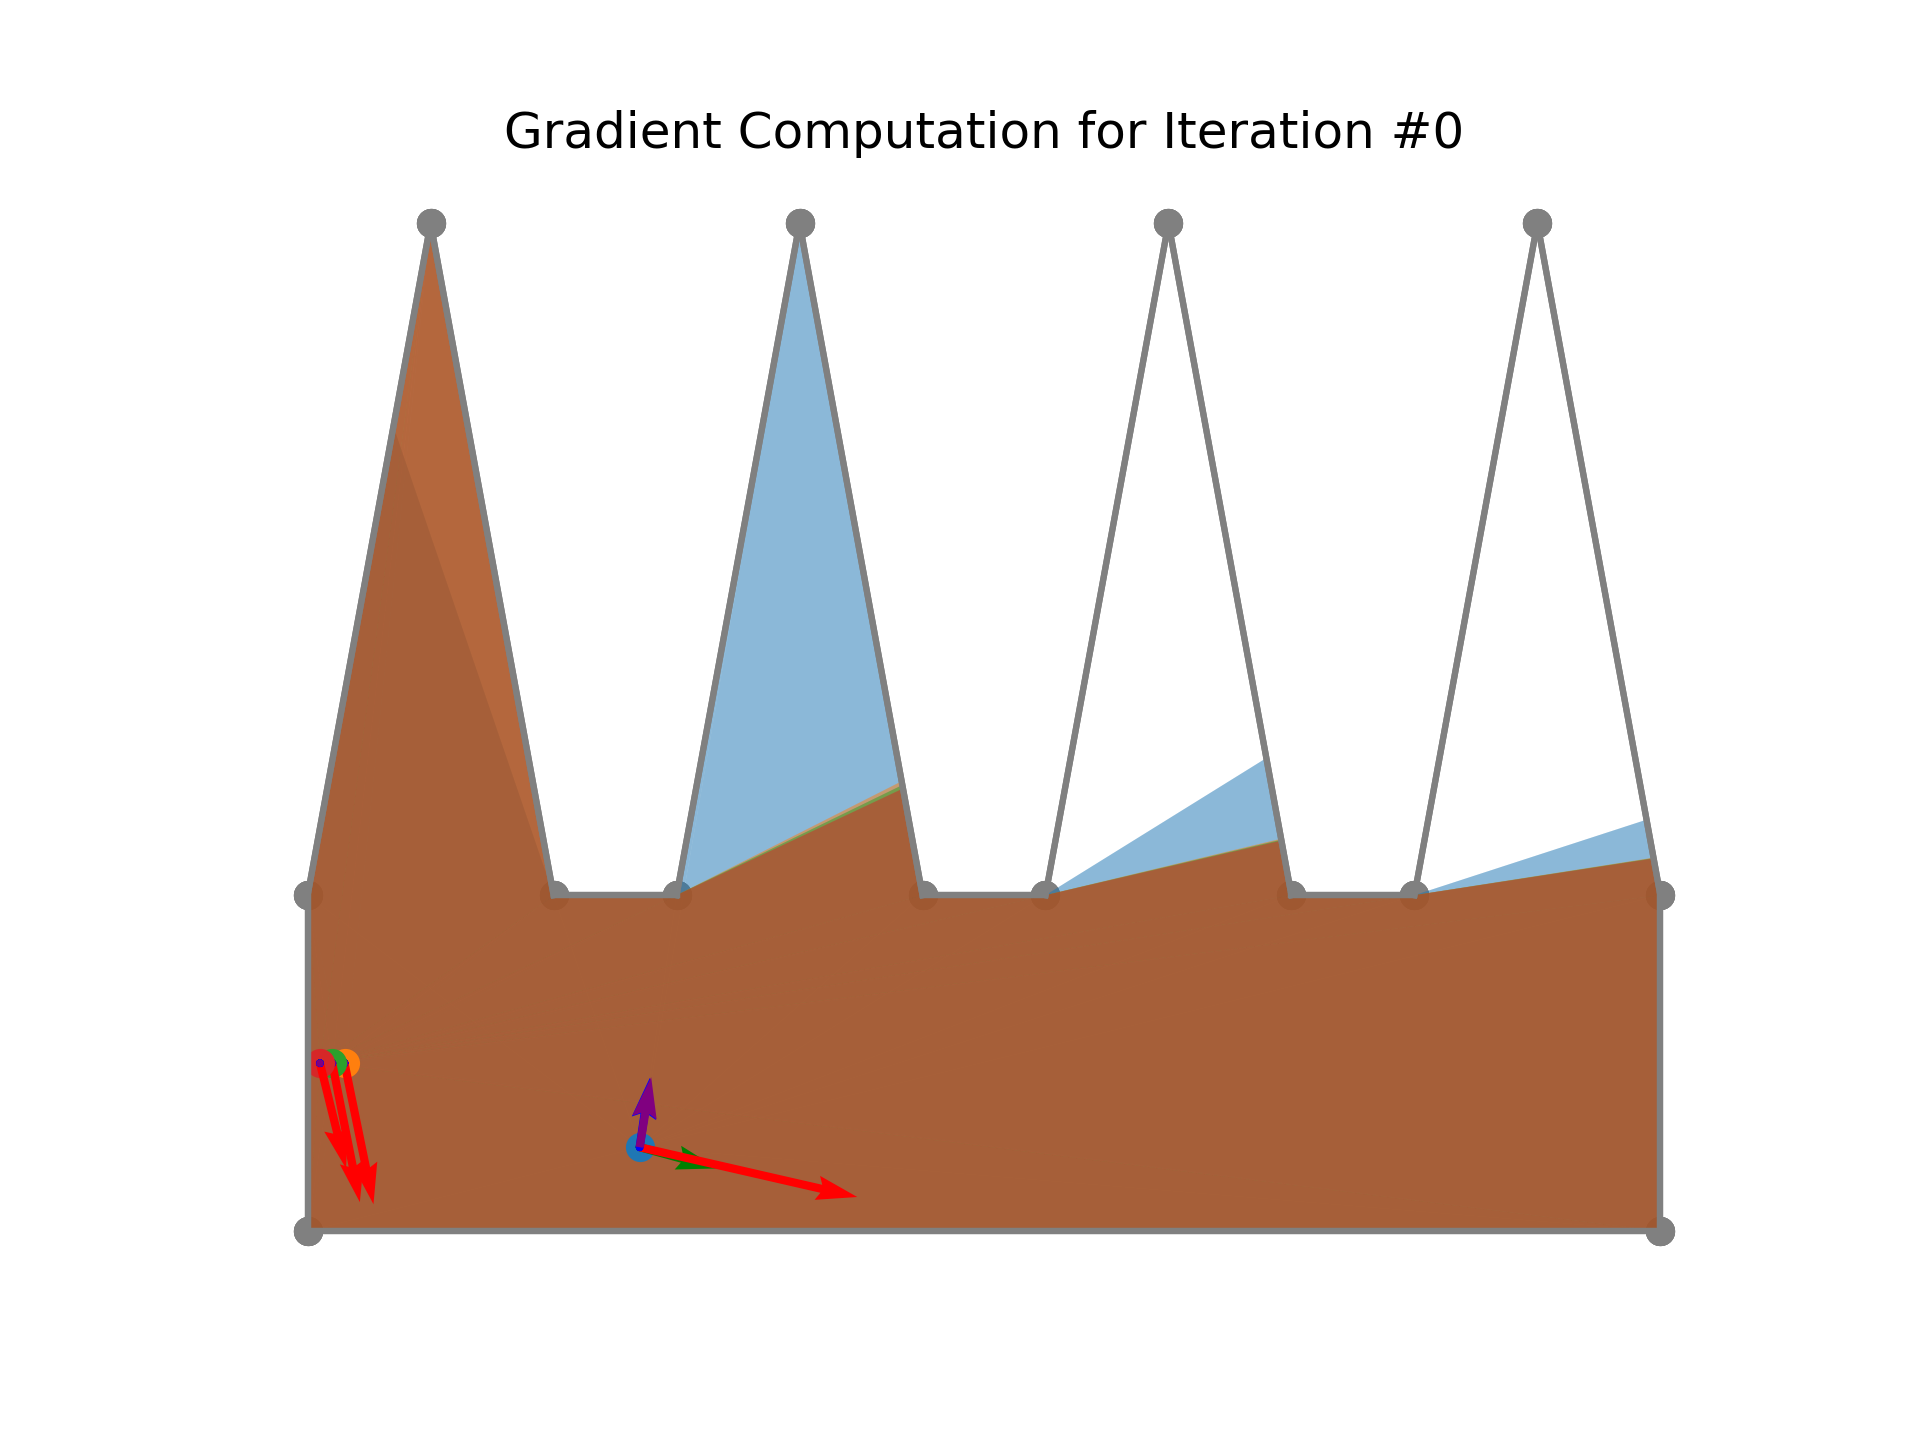
\includegraphics[width = \textwidth]{experiments/comb_capping_pos0.png}
        \caption{All heuristics, iteration 0. The guard's pull towards the reflex vertex is capped.}
        \label{fig:all_cap_pos0}
    \end{subfigure}
    \hfill
    \begin{subfigure}{0.45\textwidth}
        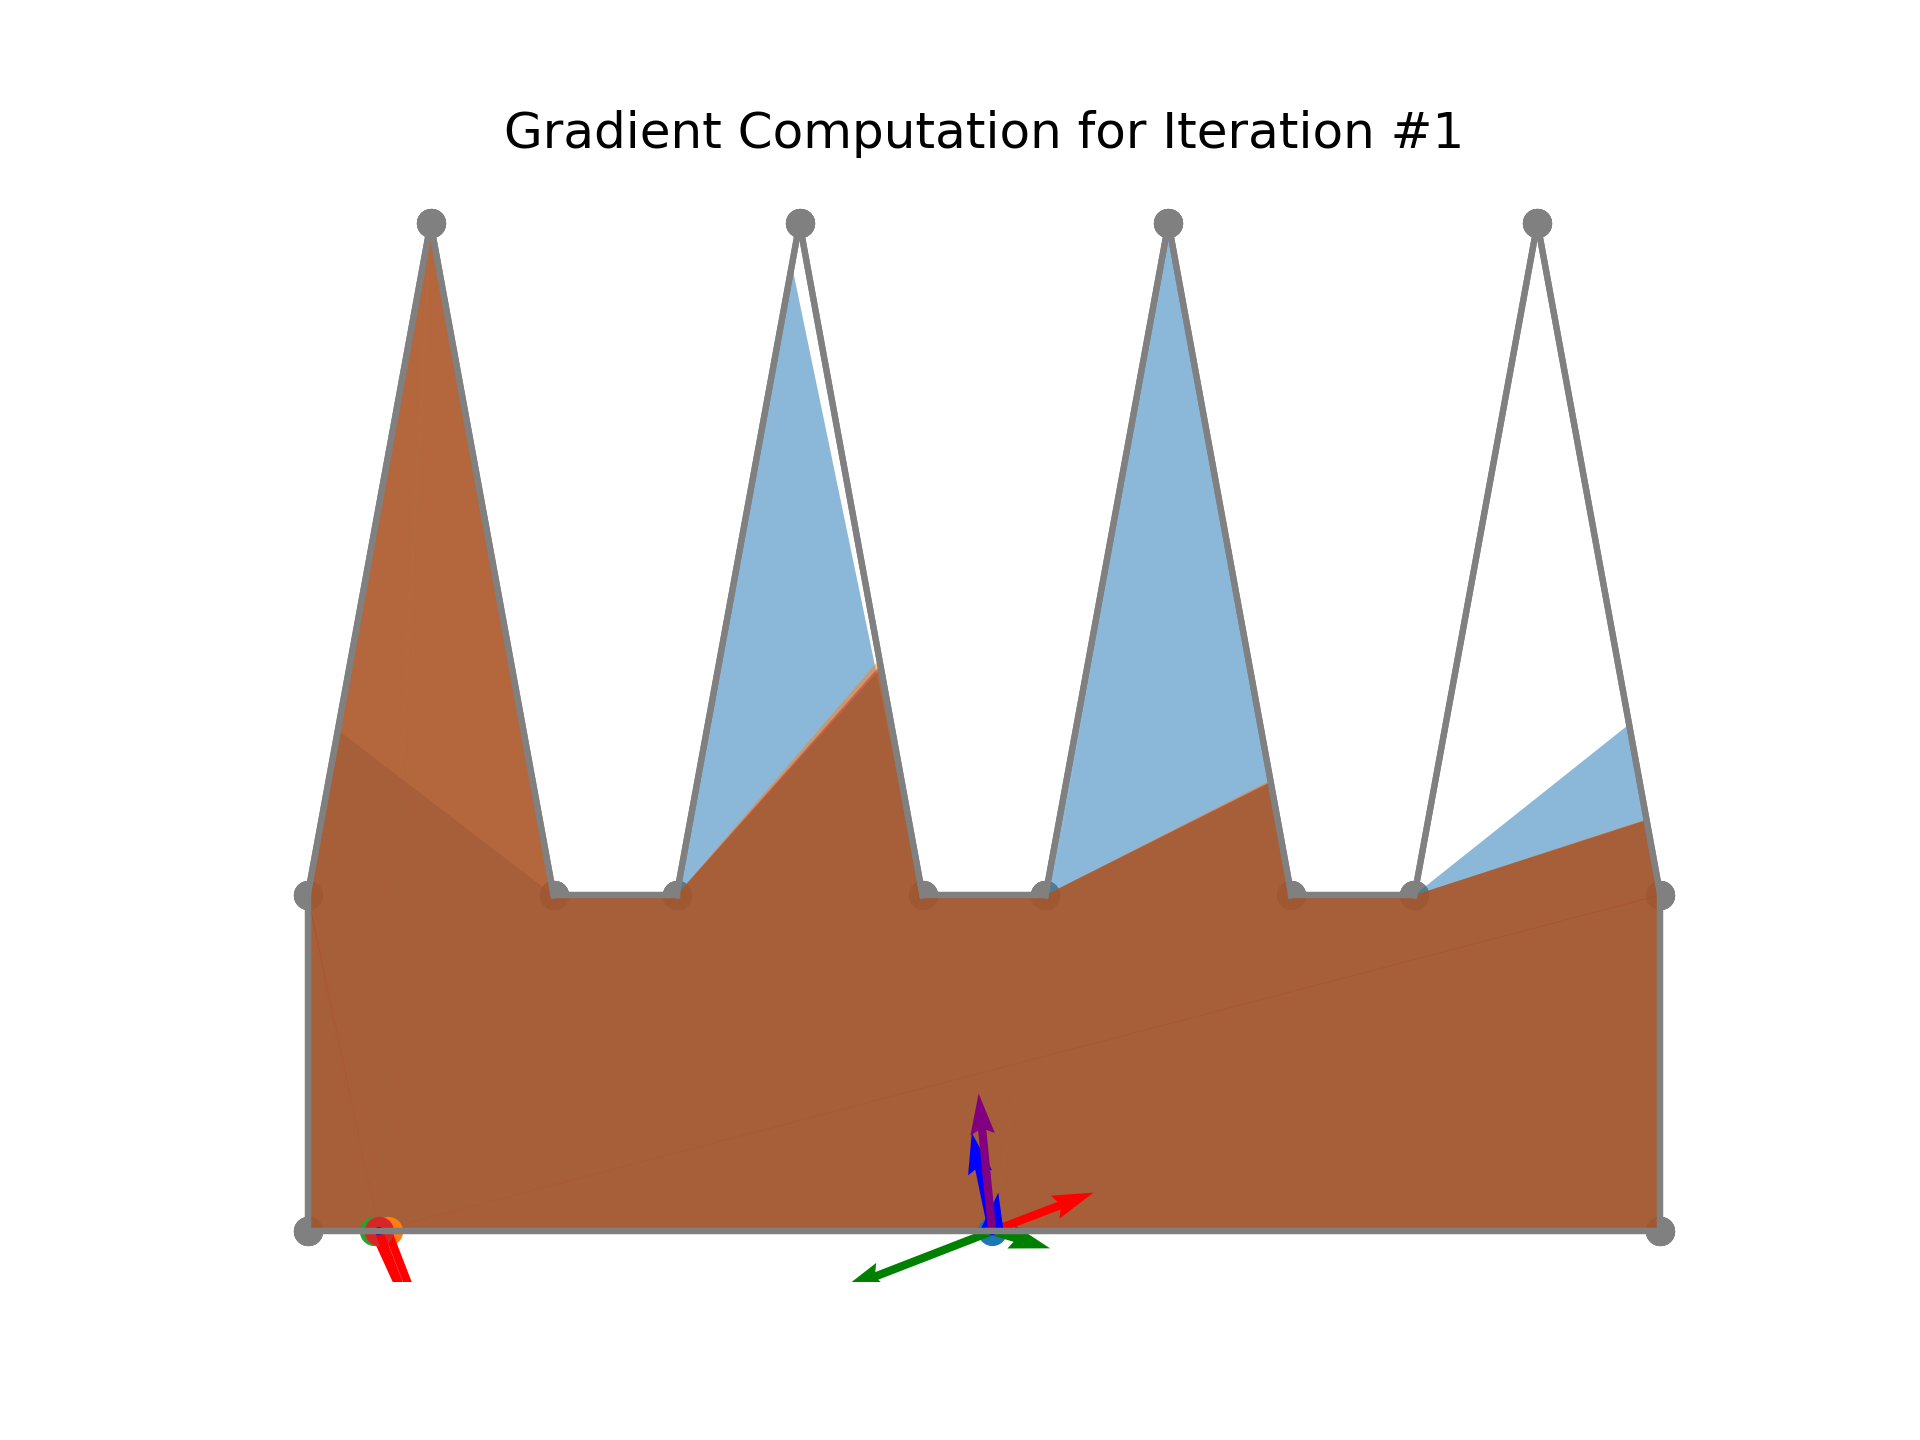
\includegraphics[width = \textwidth]{experiments/comb_capping_pos1.png}
        \caption{All heuristics, iteration 1. The guard does not act upon the pull towards the reflex vertex.}
        \label{fig:all_cap_pos1}
    \end{subfigure}
    \vfill
    \begin{subfigure}{0.45\textwidth}
        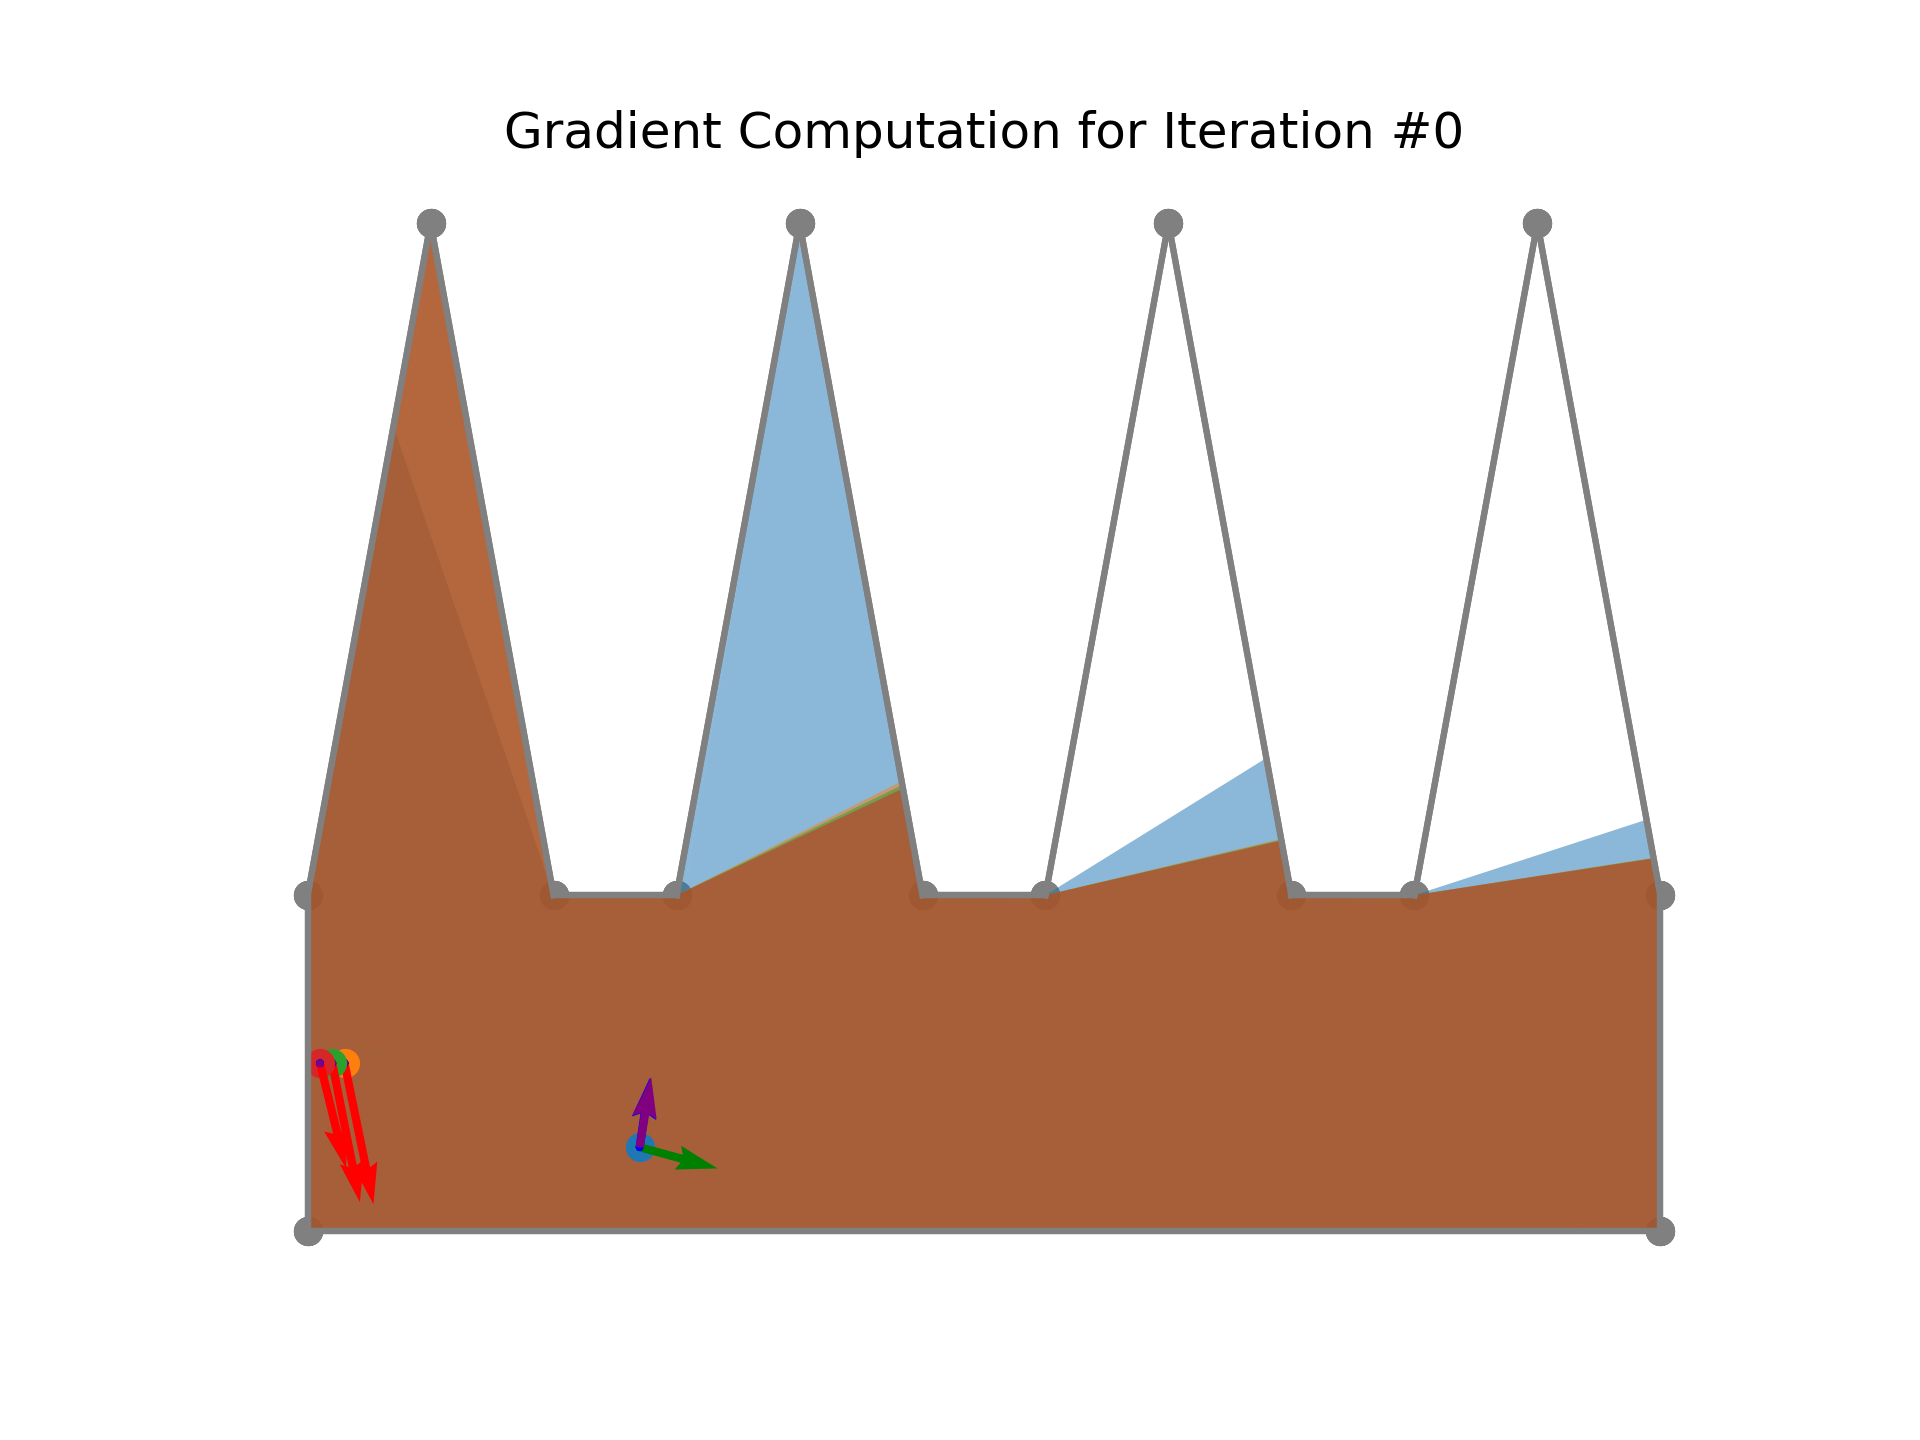
\includegraphics[width = \textwidth]{experiments/comb_no_capping_pos0.png}
        \caption{No pull onto the reflex vertex, iteration 0. The guard's pull towards the reflex vertex is not capped.}
        \label{fig:no_cap_pos0}
    \end{subfigure}
    \hfill
    \begin{subfigure}{0.45\textwidth}
        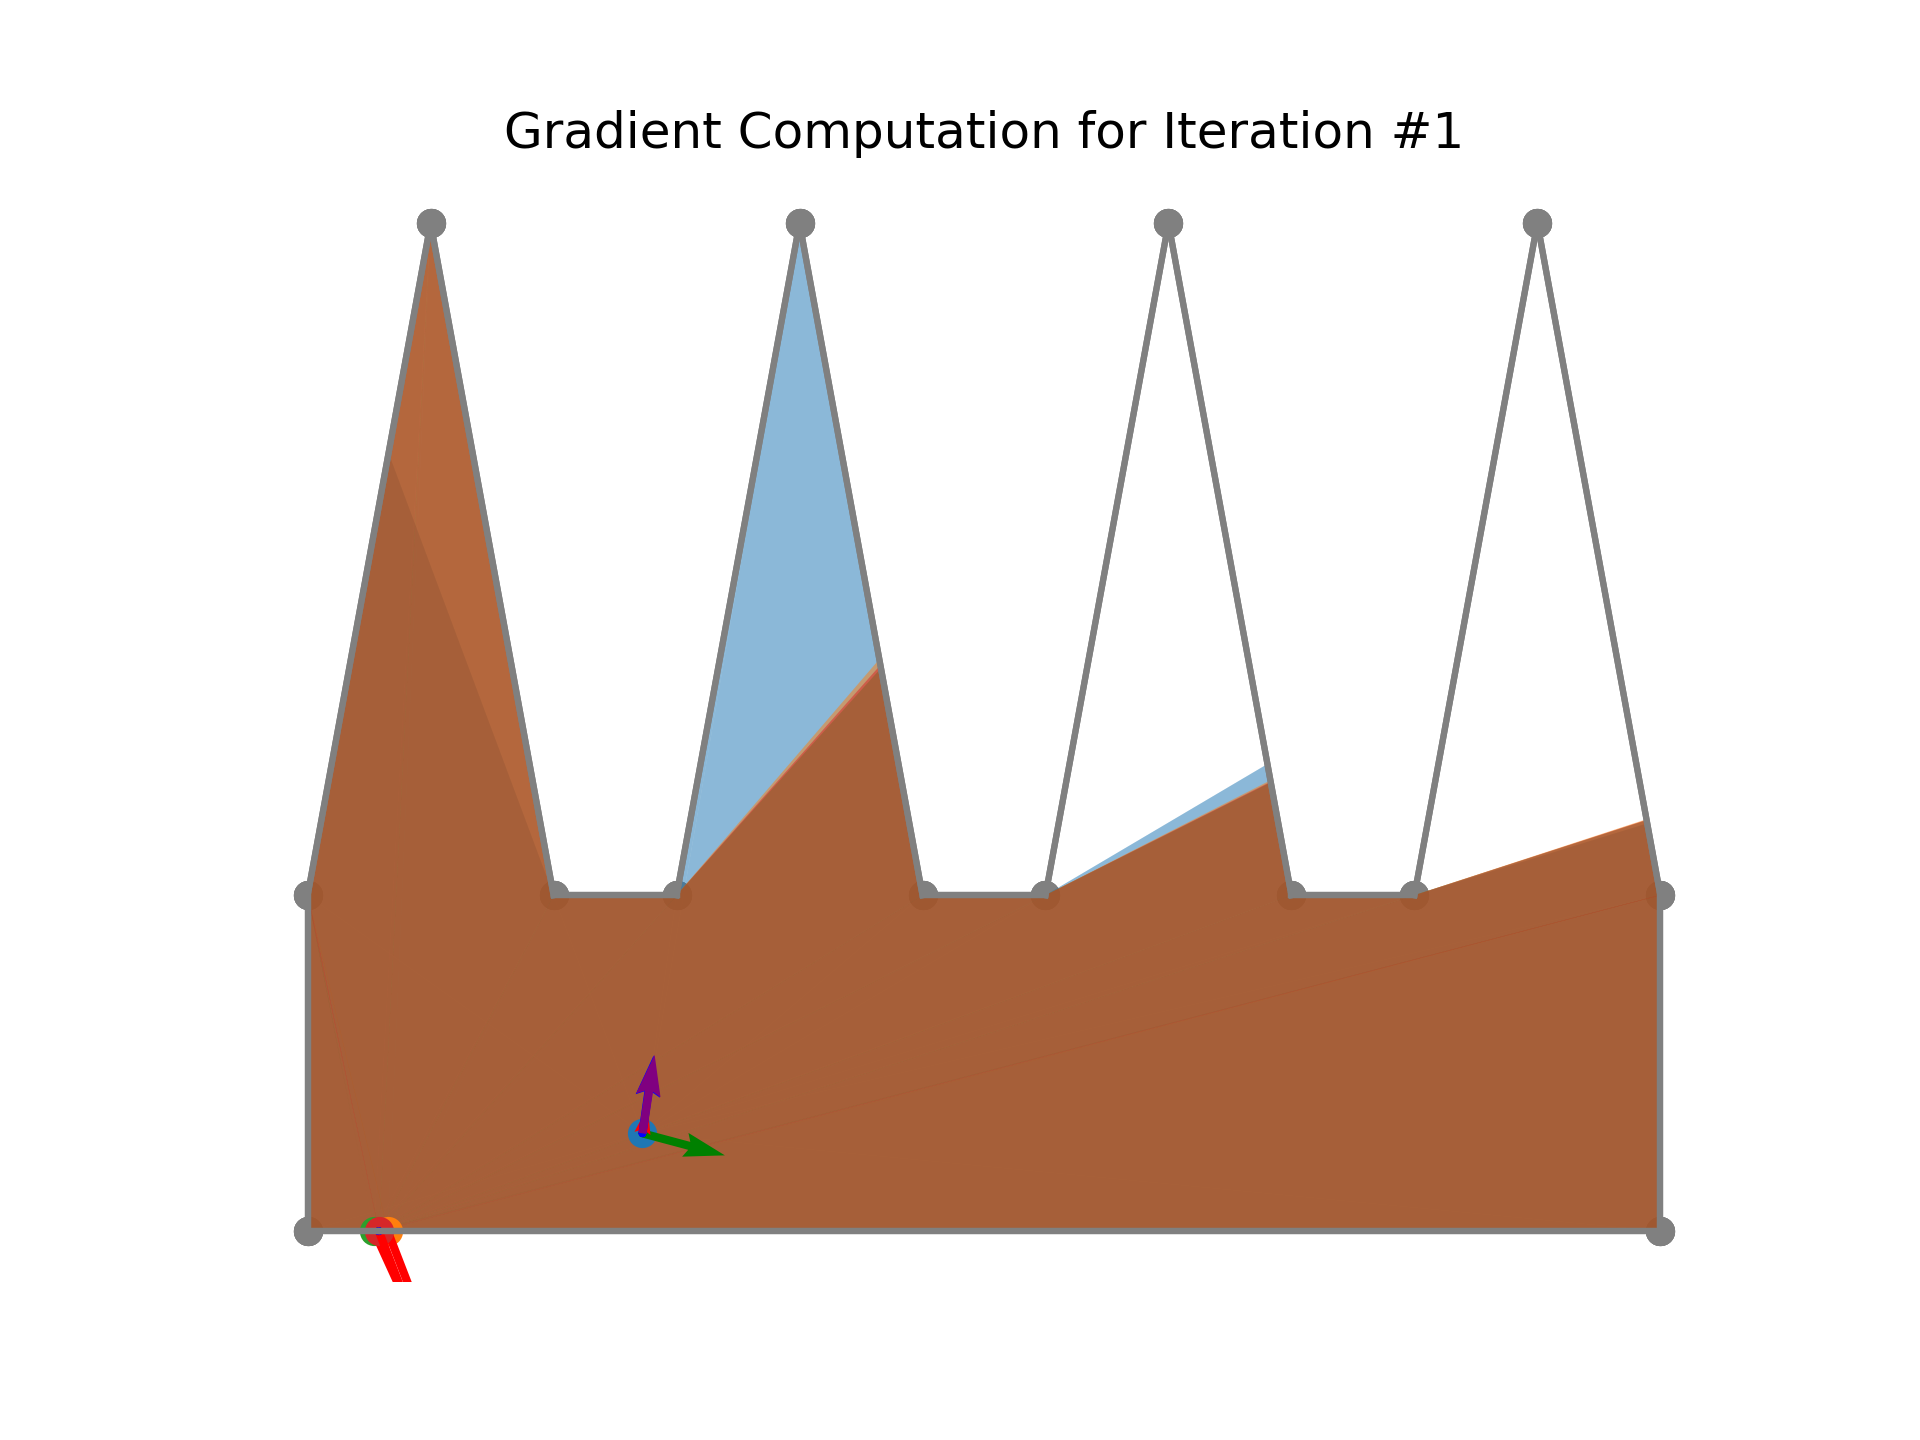
\includegraphics[width = \textwidth]{experiments/comb_no_capping_pos1.png}
        \caption{No pull onto the reflex vertex, iteration 1. The guard is drawn closer to the reflex vertex.}
        \label{fig:no_cap_pos1}
    \end{subfigure}
    \vfill
    \begin{subfigure}{0.45\textwidth}
        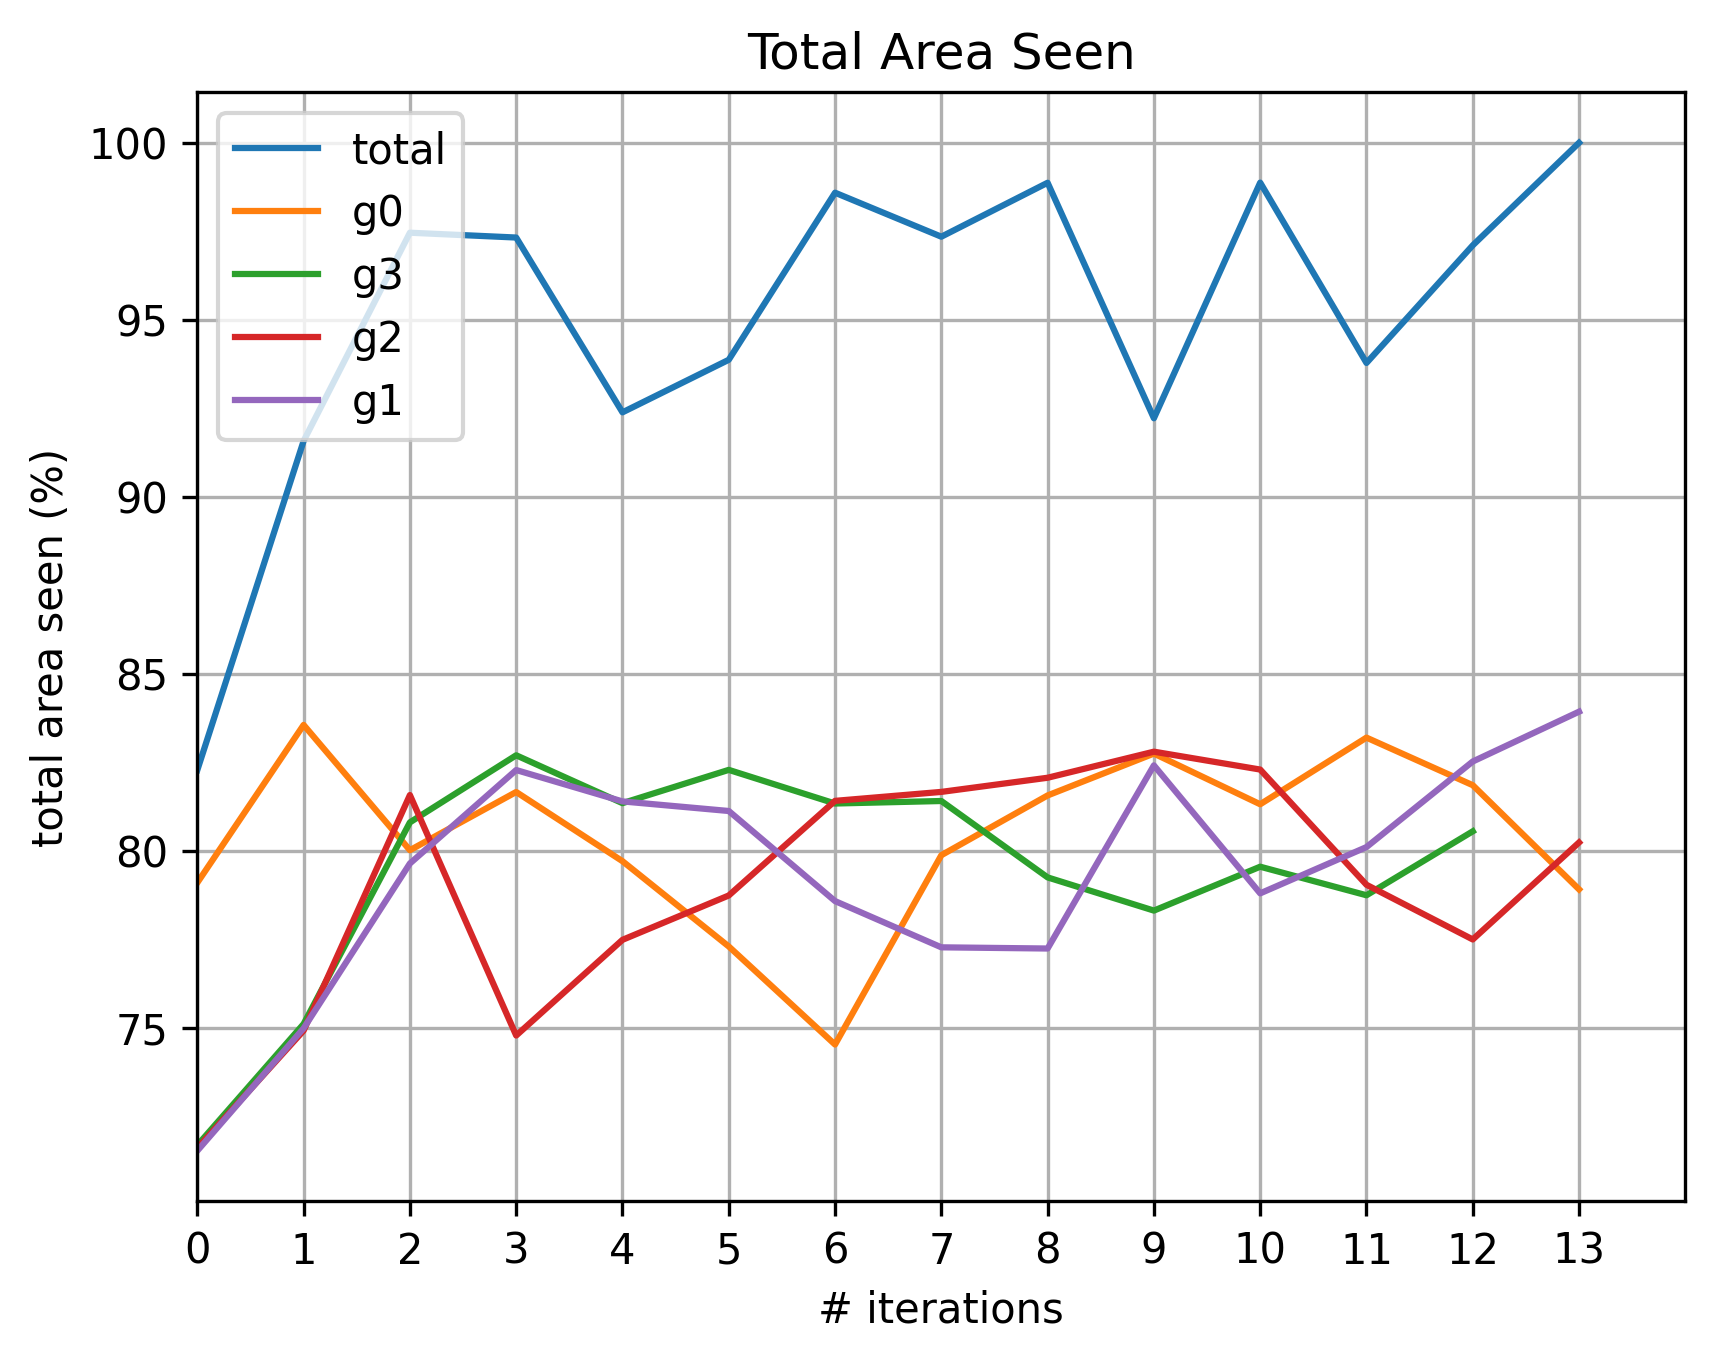
\includegraphics[width = \textwidth]{experiments/area_comb_capping.png}
        \caption{Seen area for all heuristics.}
        \label{fig:area_all_cap}
    \end{subfigure}
    \hfill
    \begin{subfigure}{0.45\textwidth}
        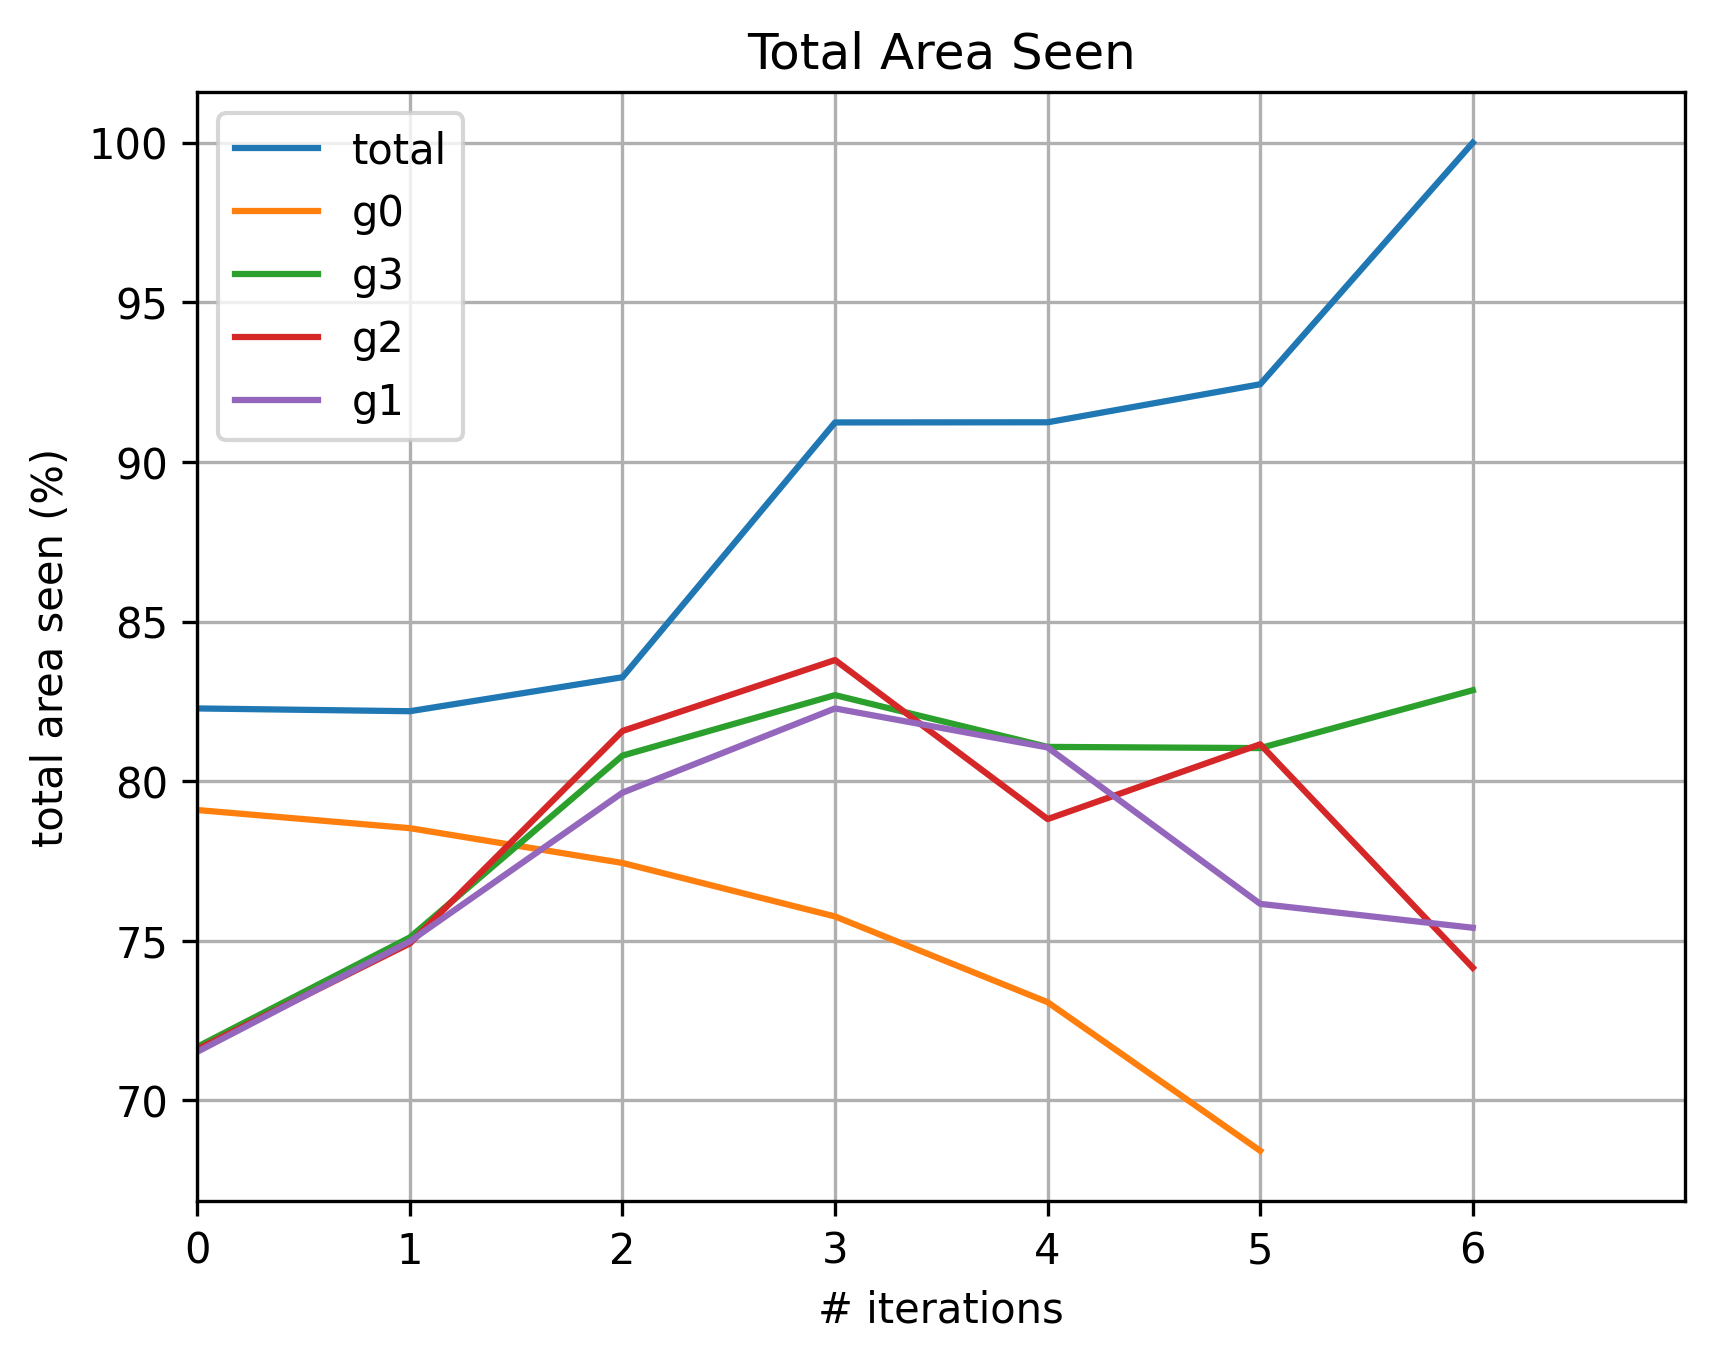
\includegraphics[width = \textwidth]{experiments/area_comb_no_capping.png}
        \caption{Seen area without pull capping.}
        \label{fig:area_no_cap}
    \end{subfigure}
    \caption{Example of different behaviours of a guard with and without its reflex vertex pull capped in a comb polygon with four teeth.}
    \label{fig:no_capping}
\end{figure}

\subsubsection{Without Reflex Area}
In this section we will discuss the importance of keeping guards in the ``reflex area'' of a reflex vertex they've been placed on. Section \ref{sec:reflex_area} introduced this heuristic. The idea is based on the fact that if guards who have been placed on reflex vertices move away from them, they might unsee some of the area they saw when on the reflex vertex. In order to prevent them from looping moving away and then back on the vertex, we will keep them in the reflex area.

We will compare how the guards move when we are using all the heuristics to when we are not keeping guards into a reflex area. We will use another arbitrary polygon as an example.

Figures \ref{fig:reflex_area_eg} and \ref{fig:area_reflex_area} compare using and not using the reflex area heuristic in terms of guard movement and total seen area, respectively. Subfigures \ref{fig:reflex_area_all1} - \ref{fig:reflex_area_all4} show the guards' movement when one of them is bound to the reflex area. In this case, because the blue guard wants to move away from the reflex vertex, the reflex area does not allow it to move away from the reflex vertex. So, it stays there. 
Subfigures \ref{fig:reflex_area_no1} - \ref{fig:reflex_area_no4} display the guards' movement when the reflex area heuristic is not applied. In this case, the blue guard moves away from the reflex vertex (Subfigure \ref{fig:reflex_area_no2}), to be drawn back to it in the next iteration (Subfigure \ref{fig:reflex_area_no3}). This repetitive behaviour continues without allowing the polygon to be completely seen.

\begin{figure}[h!]
    \centering
    \begin{subfigure}{0.45\textwidth}
        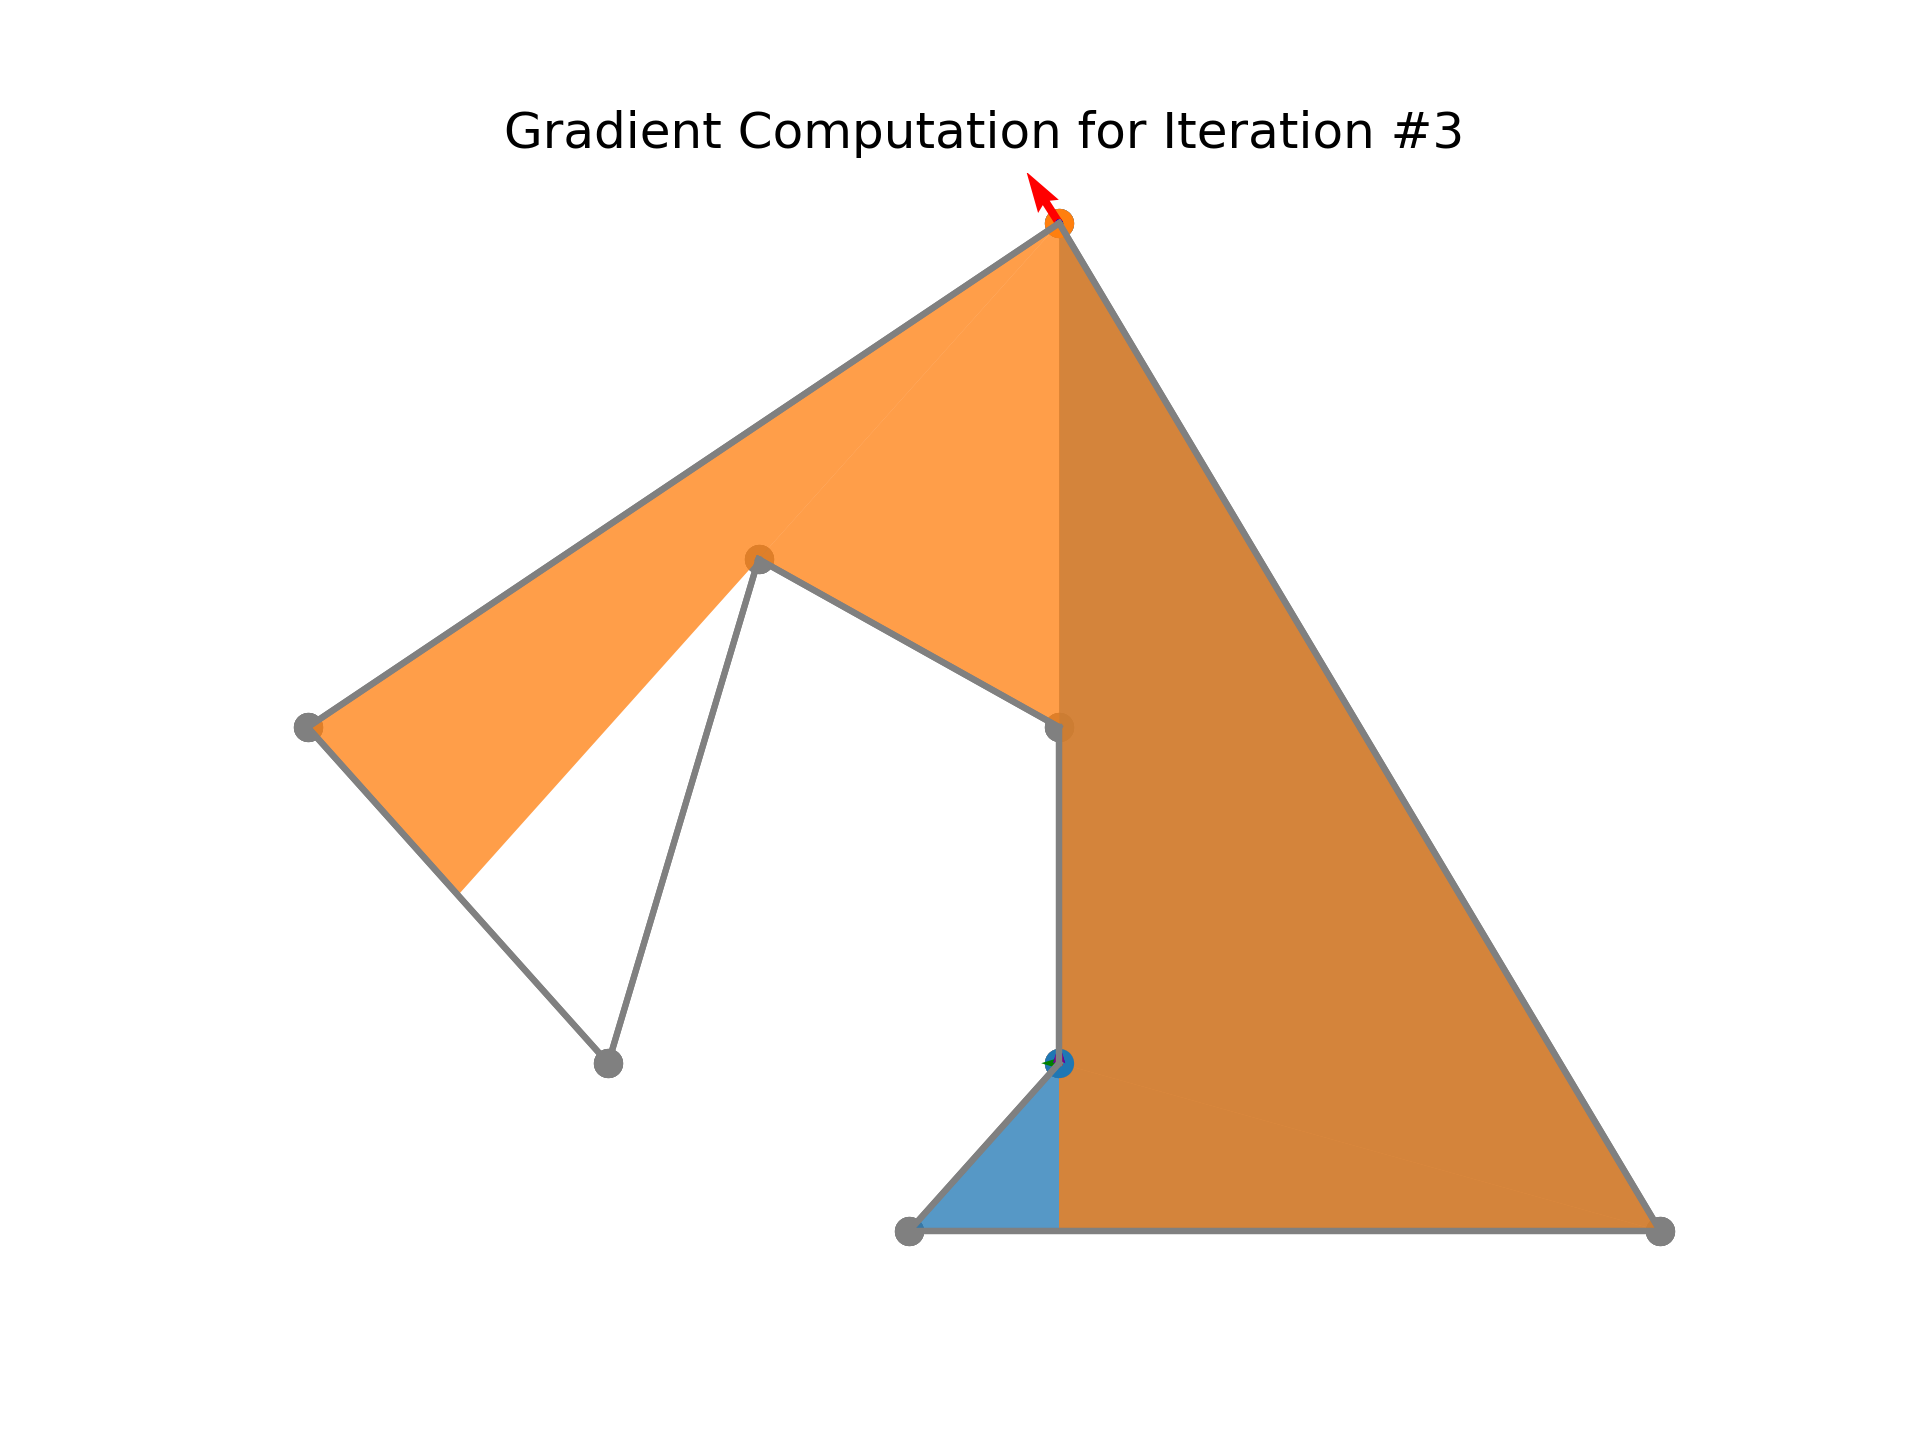
\includegraphics[width = \textwidth]{experiments/reflex_area_all_pos3.png}
        \caption{All heuristics, iteration 3. The blue guard is on the reflex vertex.}
        \label{fig:reflex_area_all1}
    \end{subfigure}
    \hfill
    \begin{subfigure}{0.45\textwidth}
        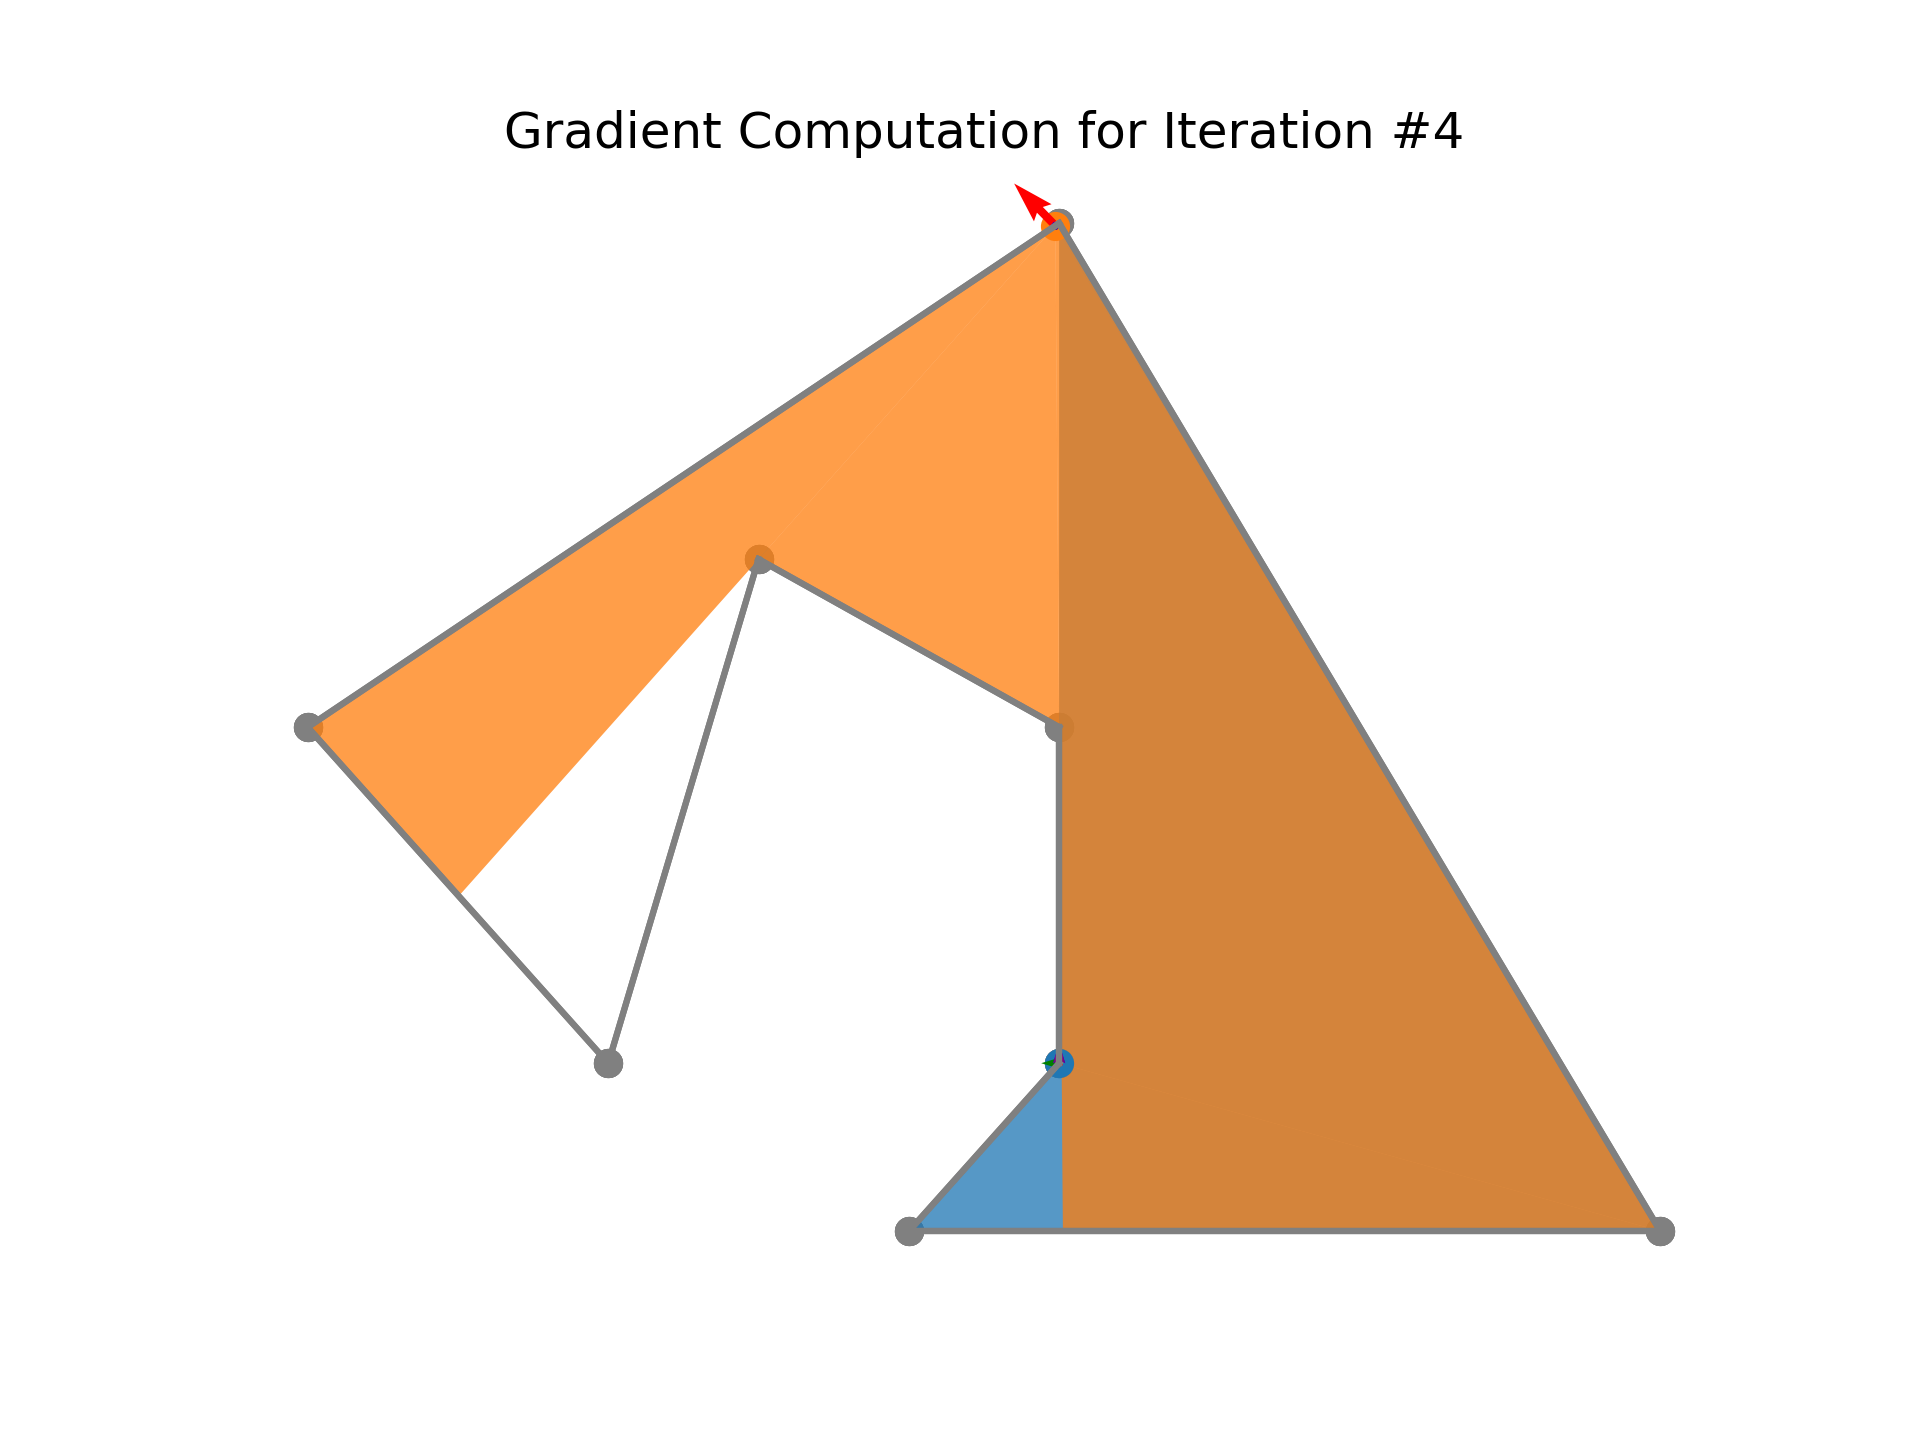
\includegraphics[width = \textwidth]{experiments/reflex_area_all_pos4.png}
        \caption{All heuristics, iteration 4. The blue guard is still on the reflex vertex (in the reflex area).}
    \end{subfigure}
    \hfill
    \begin{subfigure}{0.45\textwidth}
        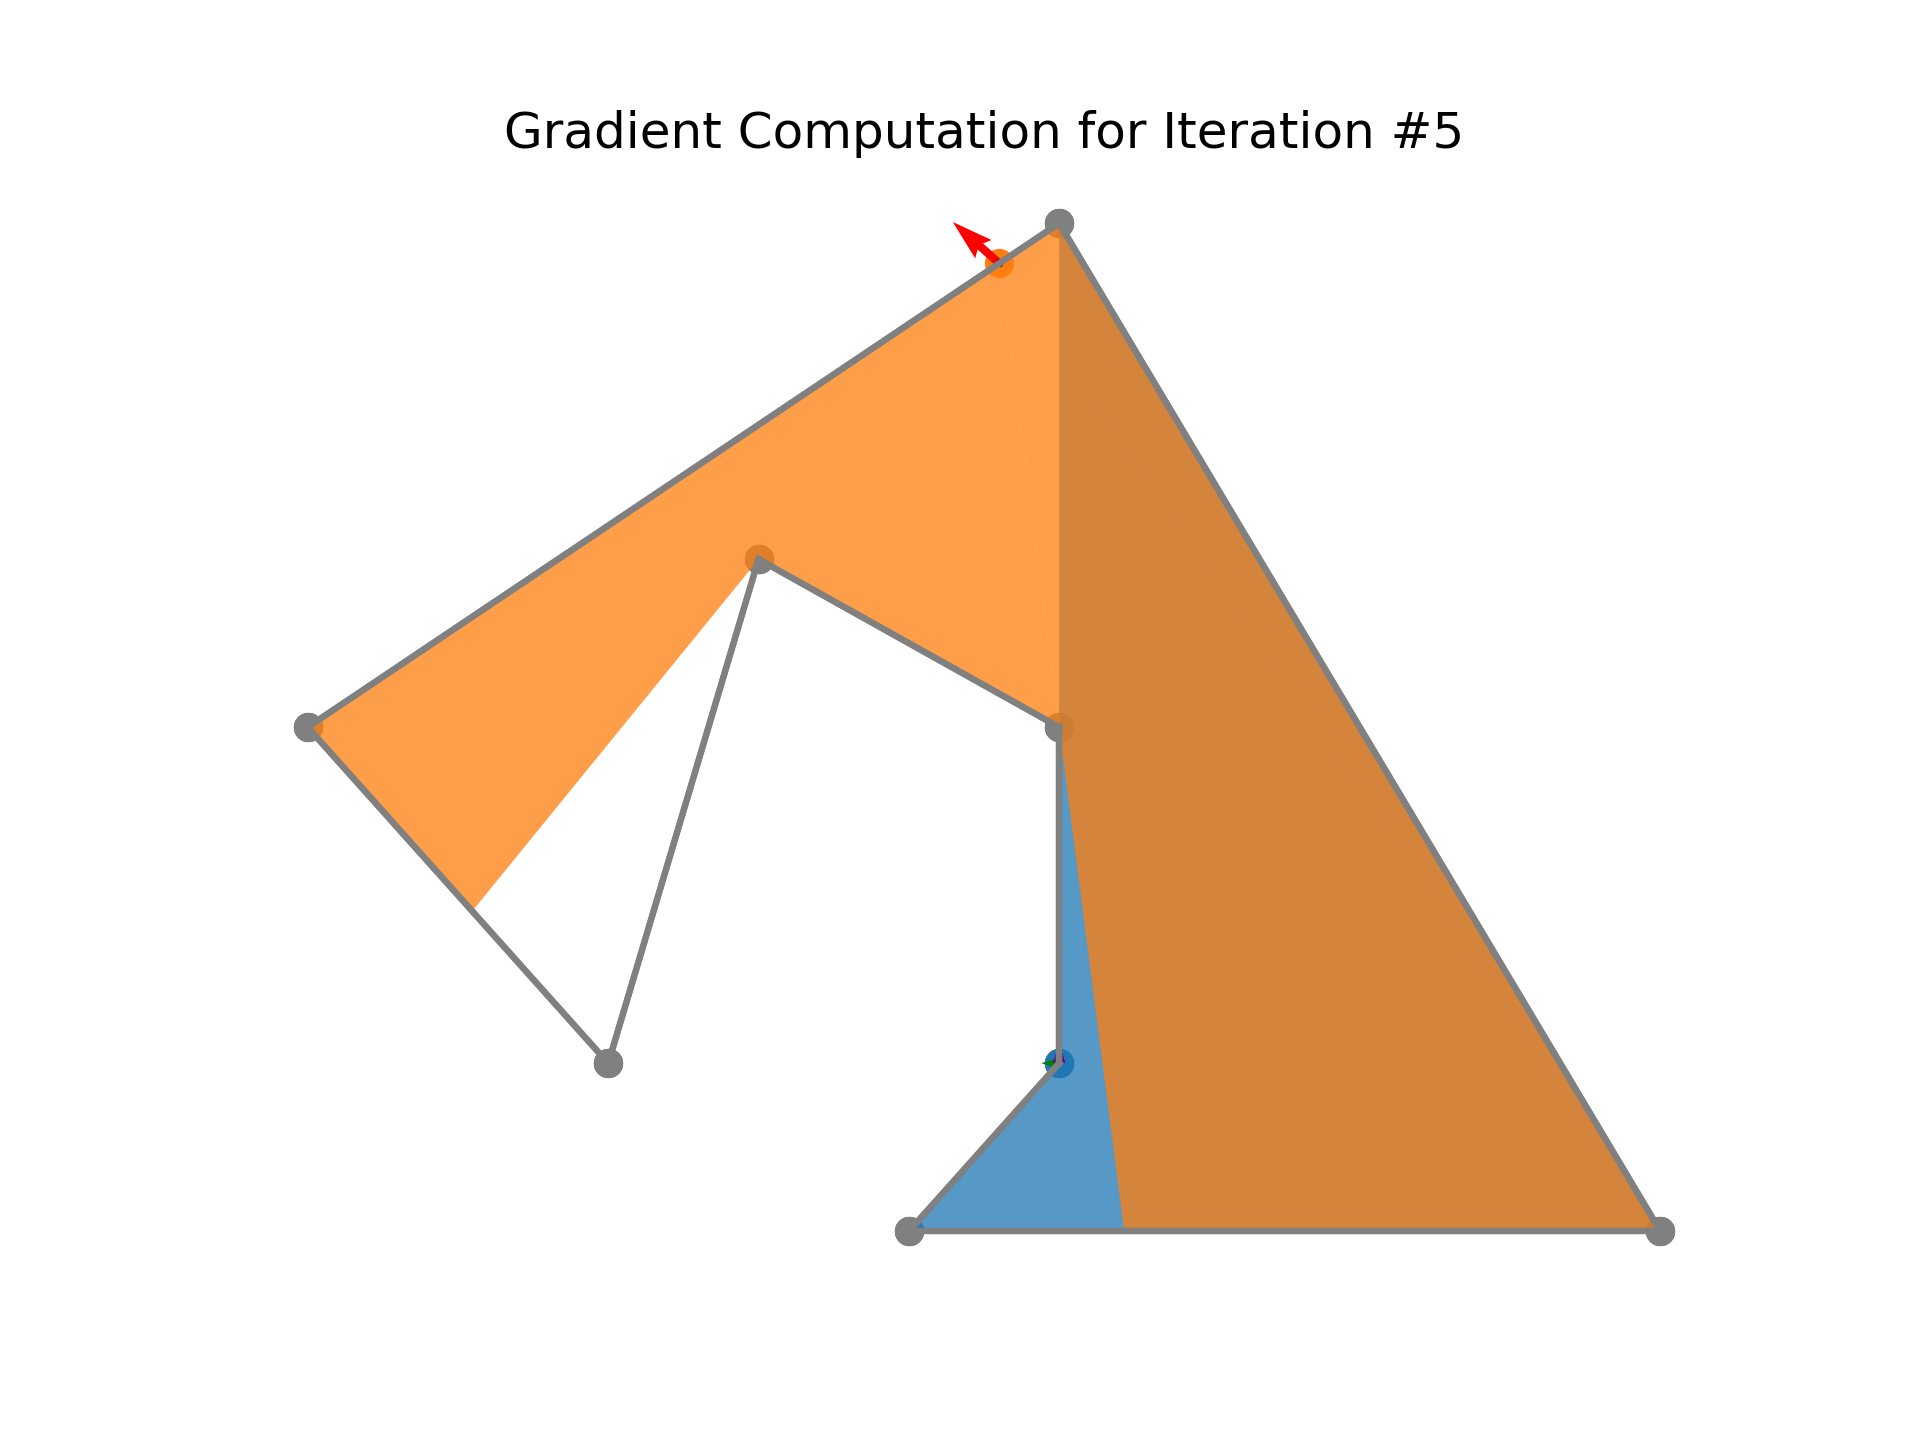
\includegraphics[width = \textwidth]{experiments/reflex_area_all_pos5.png}
        \caption{All heuristics, iteration 5. The blue guard is still on the reflex vertex (in the reflex area).}
    \end{subfigure}
    \hfill
    \begin{subfigure}{0.45\textwidth}
        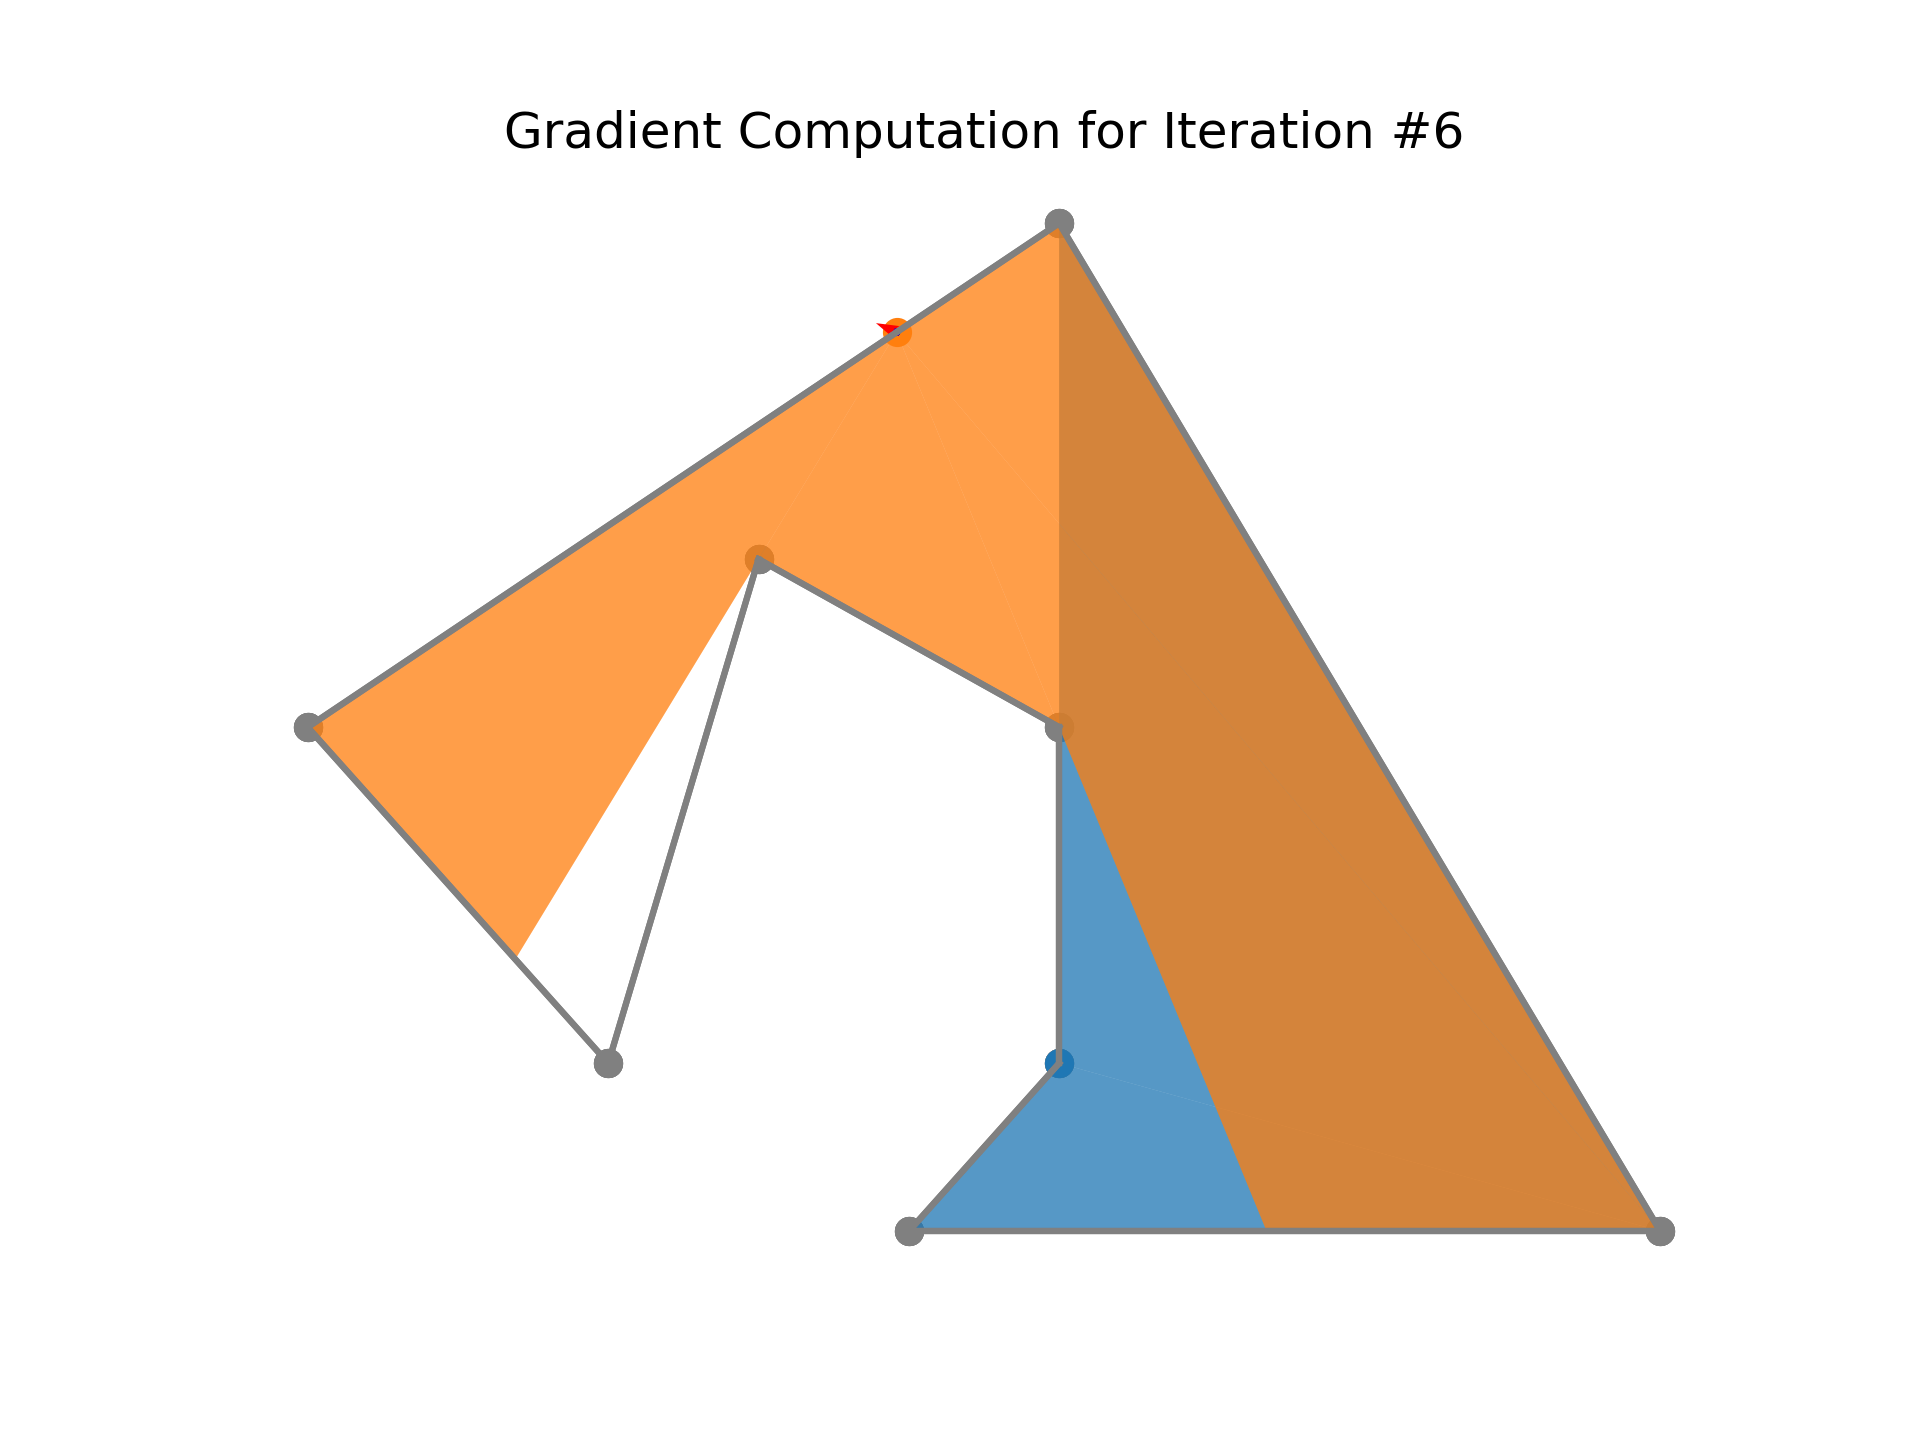
\includegraphics[width = \textwidth]{experiments/reflex_area_all_pos6.png}
        \caption{All heuristics, iteration 6. The blue guard is still on the reflex vertex (in the reflex area).}
        \label{fig:reflex_area_all4}
    \end{subfigure}
    \begin{subfigure}{0.45\textwidth}
        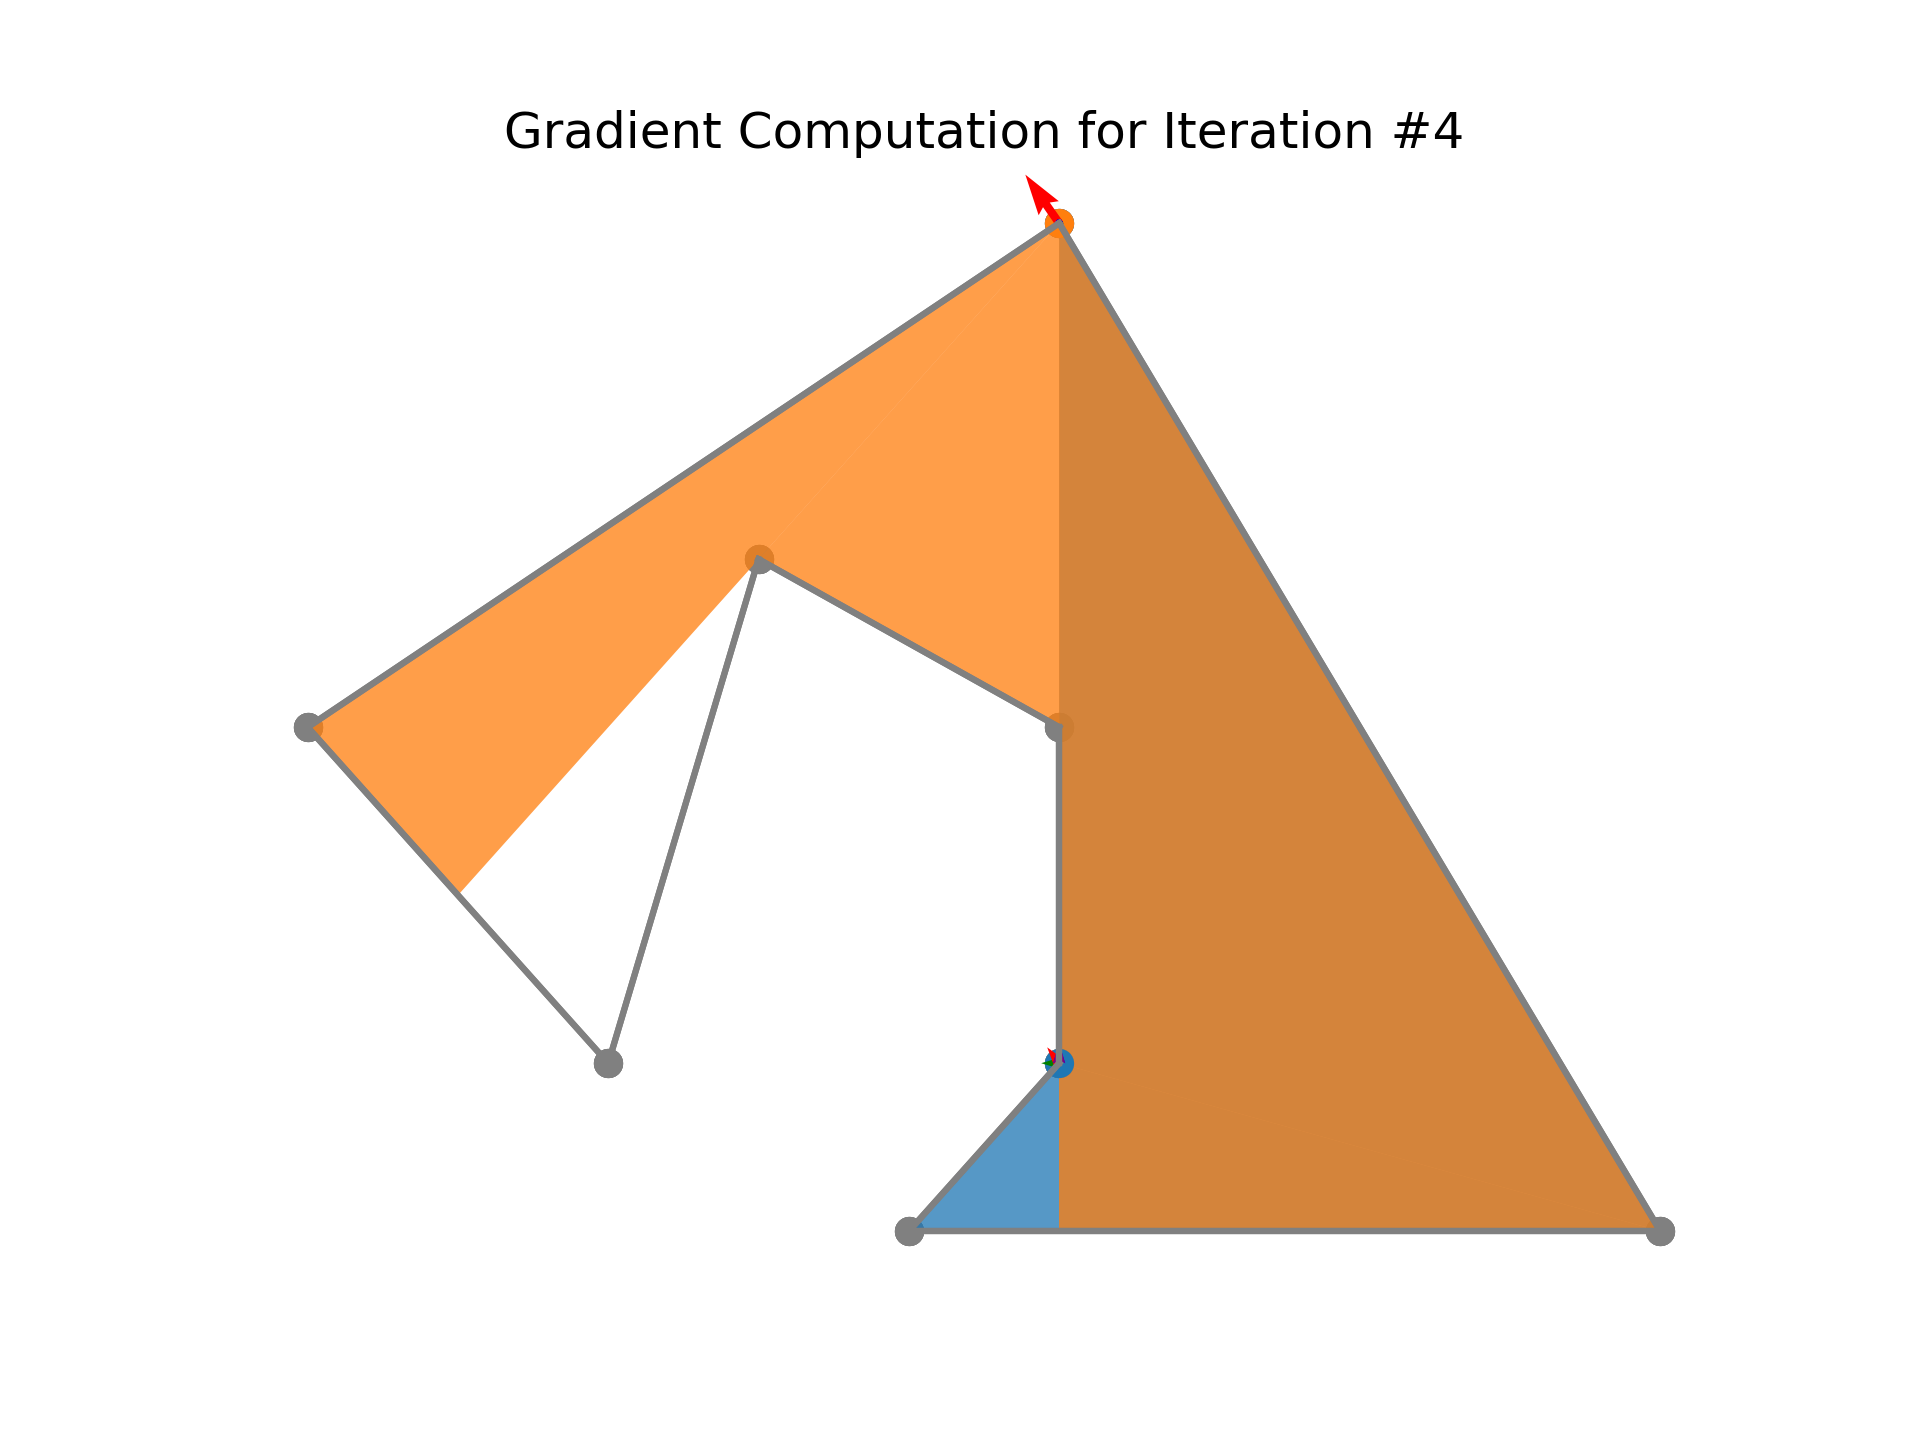
\includegraphics[width = \textwidth]{experiments/reflex_area_no_pos4.png}
        \caption{No reflex area, iteration 4. The blue guard is on the reflex vertex.}
        \label{fig:reflex_area_no1}
    \end{subfigure}
    \hfill
    \begin{subfigure}{0.45\textwidth}
        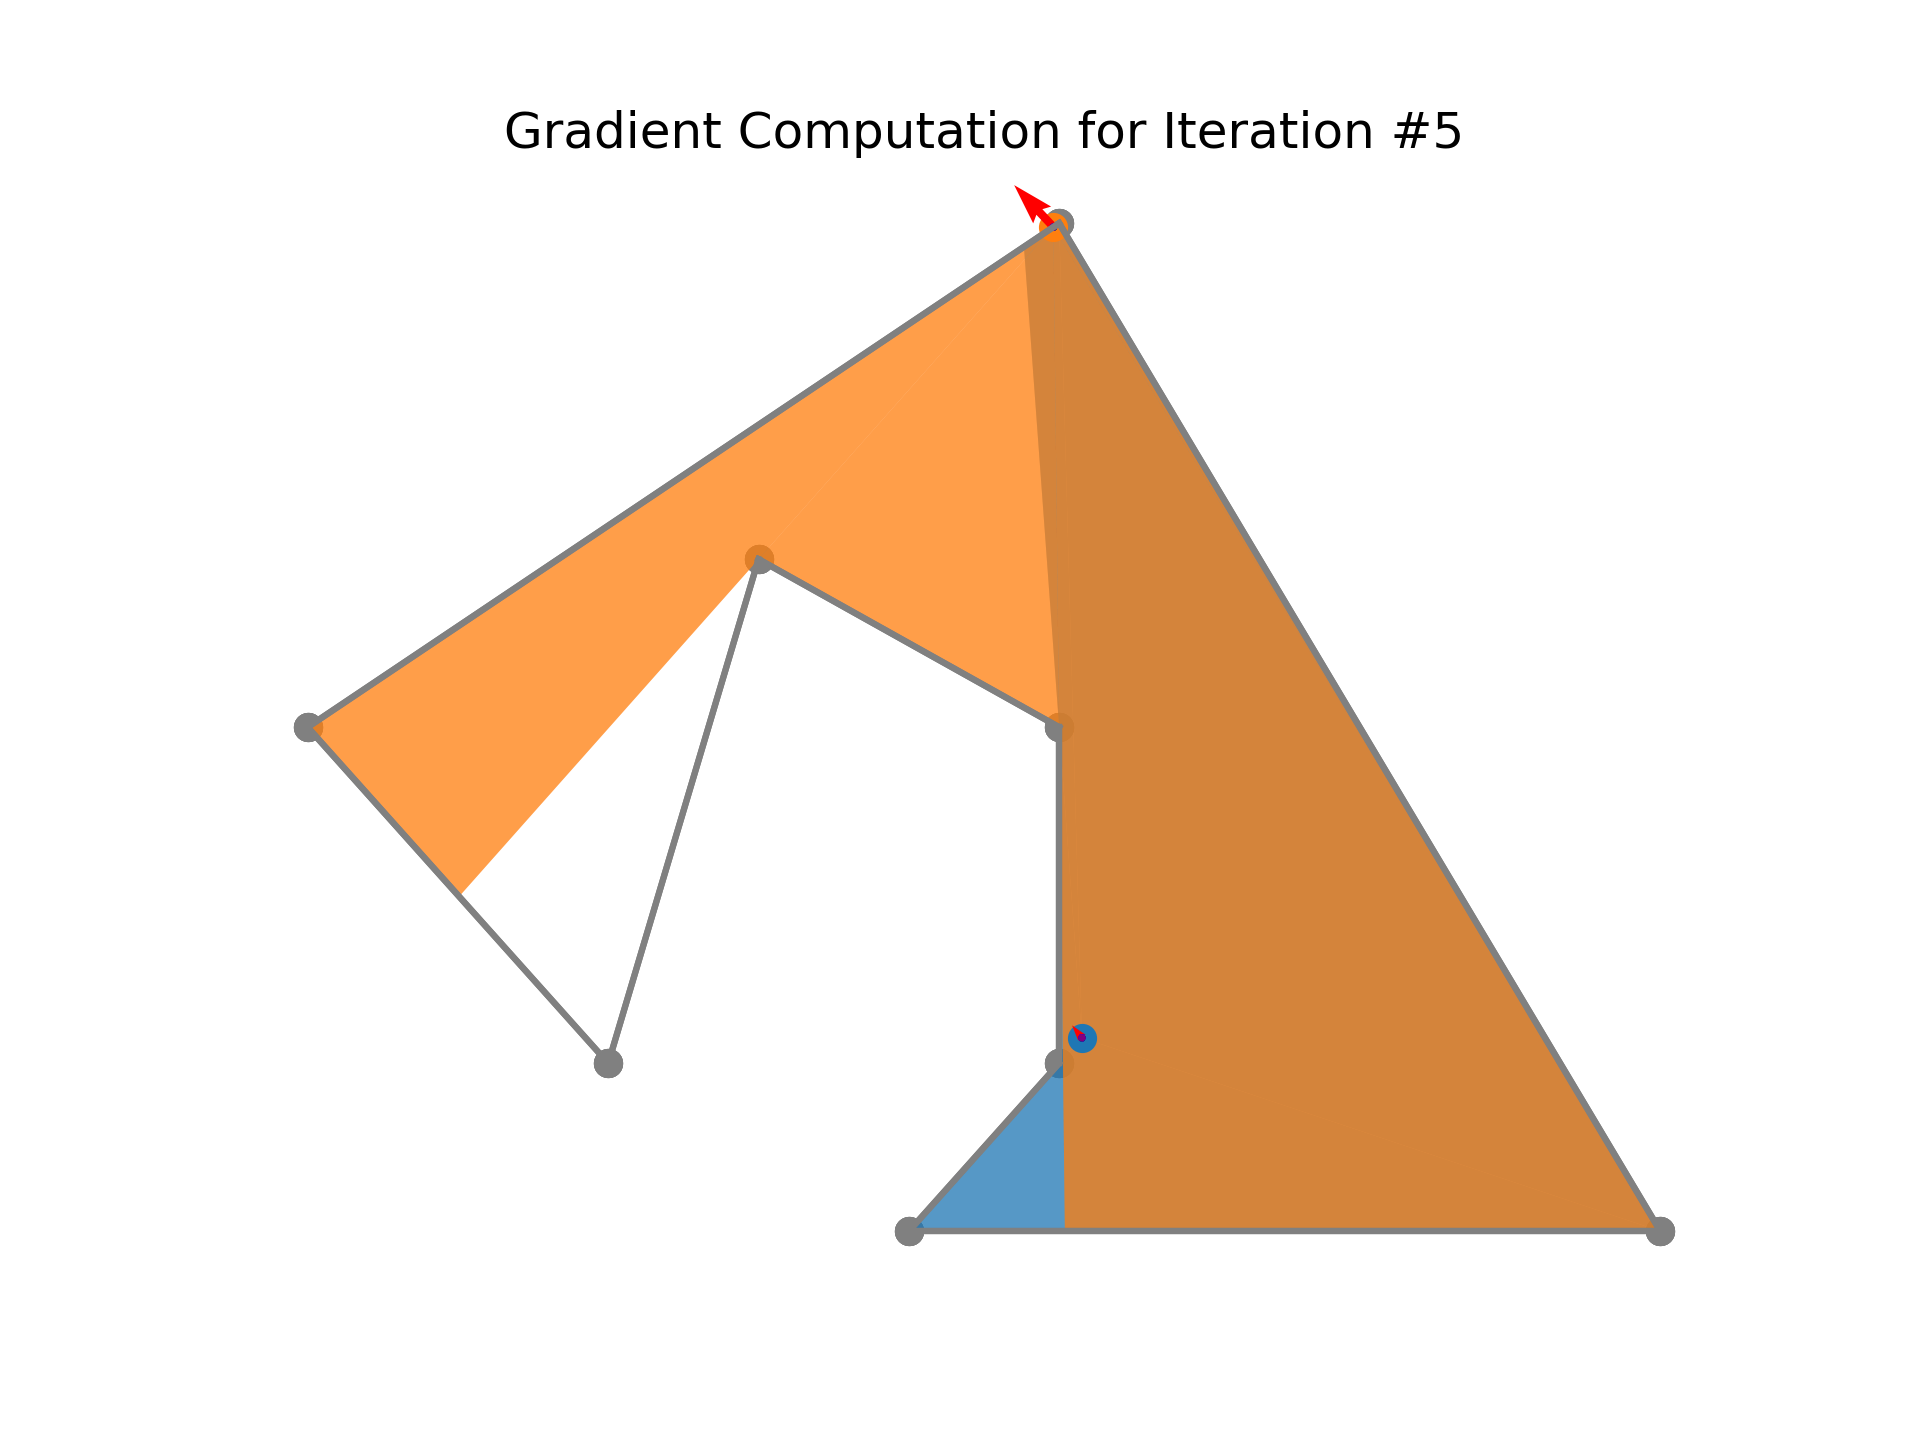
\includegraphics[width = \textwidth]{experiments/reflex_area_no_pos5.png}
        \caption{No reflex area, iteration 5. The blue guard moved away from the reflex vertex.}
        \label{fig:reflex_area_no2}
    \end{subfigure}
    \hfill
    \begin{subfigure}{0.45\textwidth}
        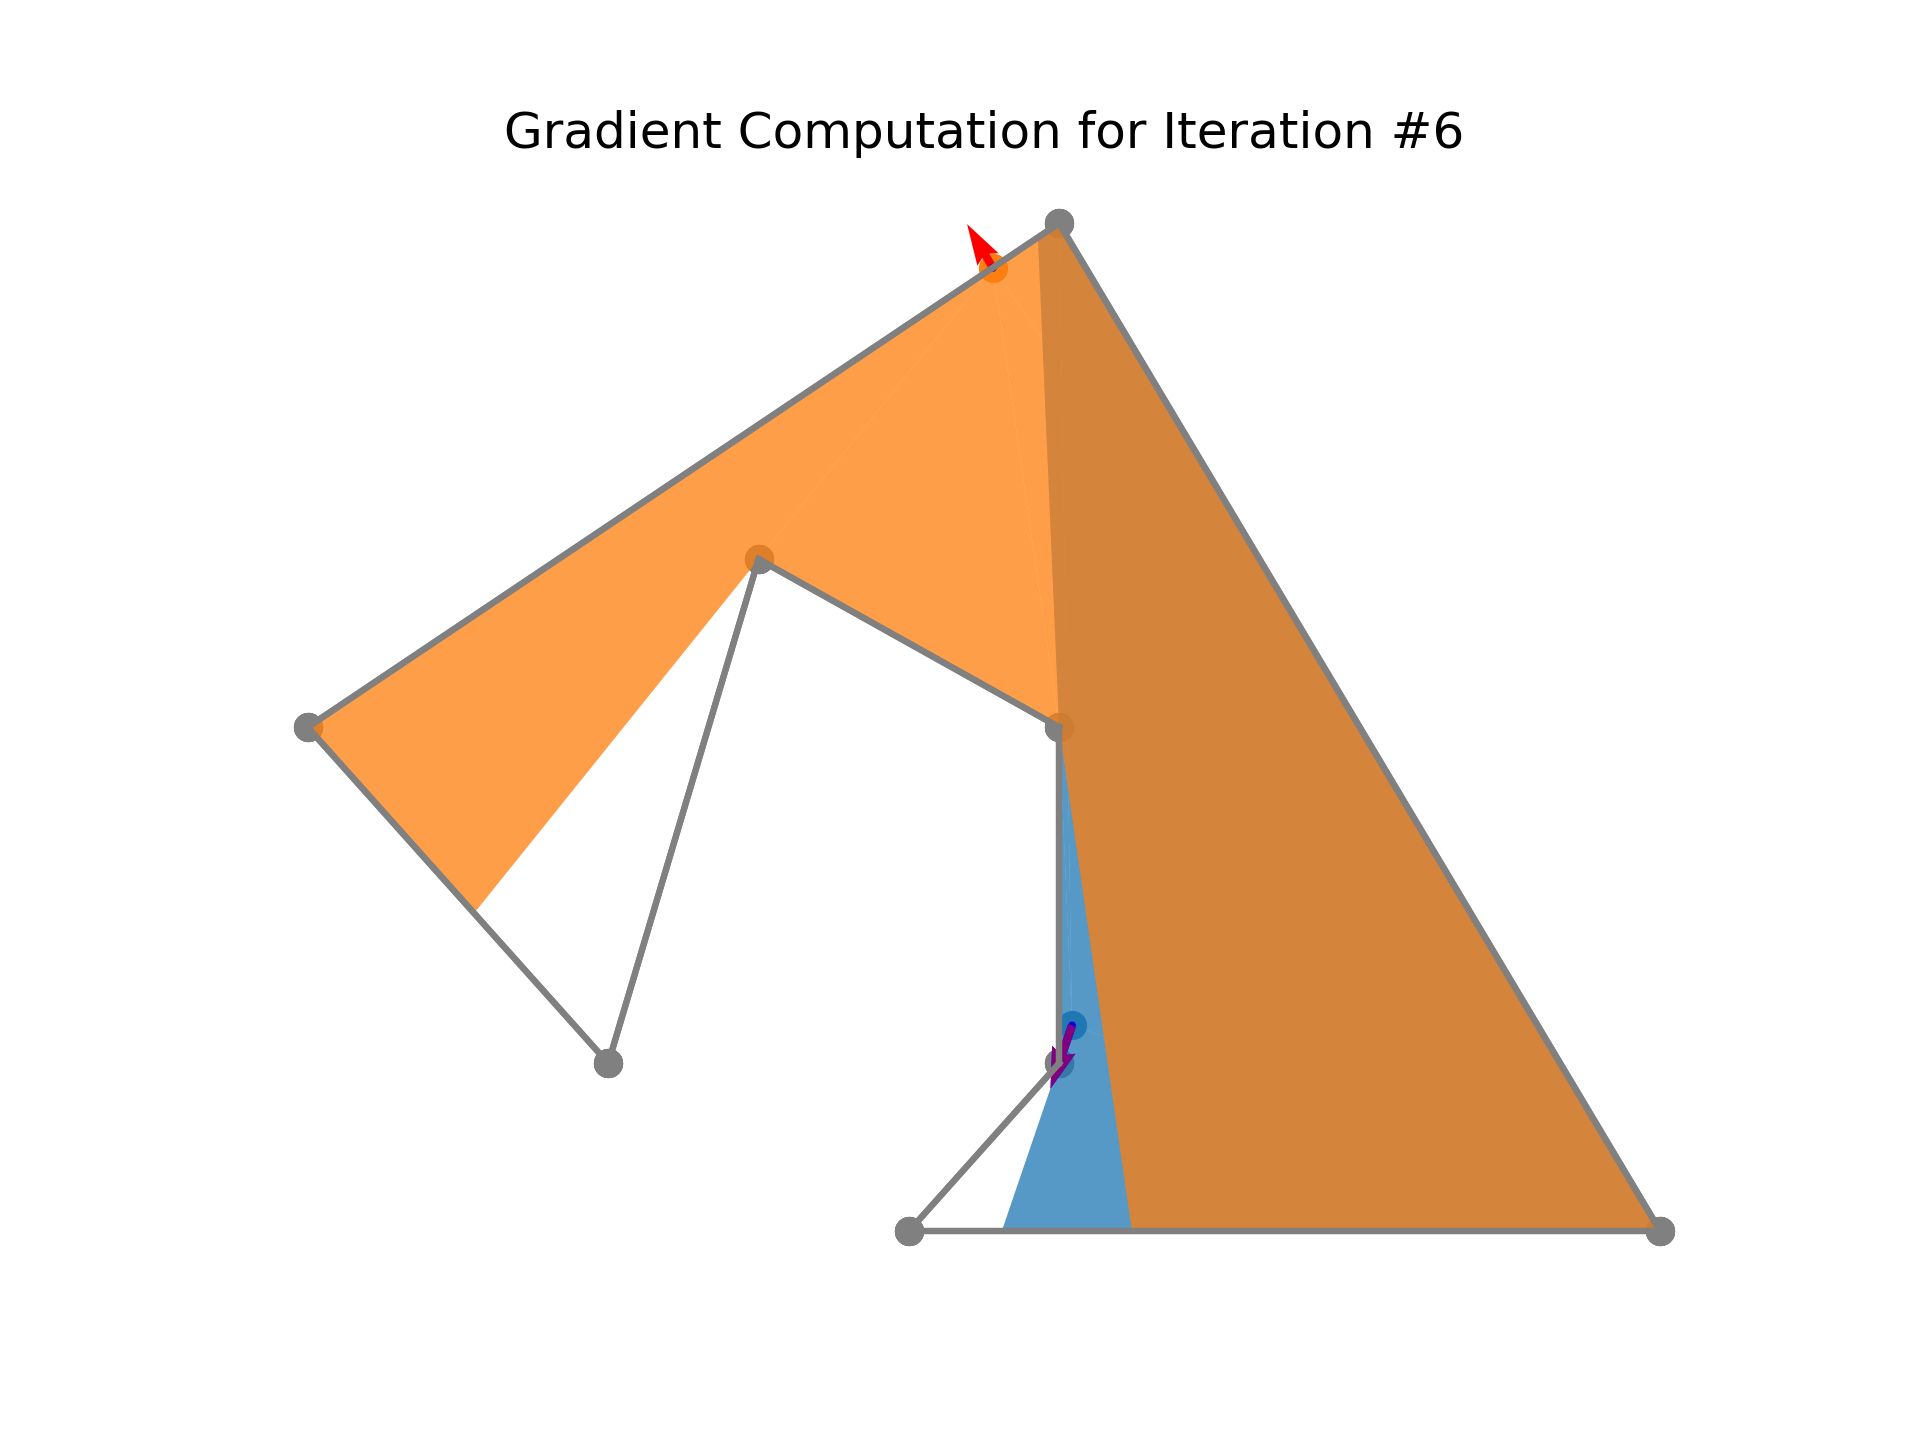
\includegraphics[width = \textwidth]{experiments/reflex_area_no_pos6.png}
        \caption{No reflex area, iteration 6. The blue guard is drawn back to the same reflex vertex.}
        \label{fig:reflex_area_no3}
    \end{subfigure}
    \hfill
    \begin{subfigure}{0.45\textwidth}
        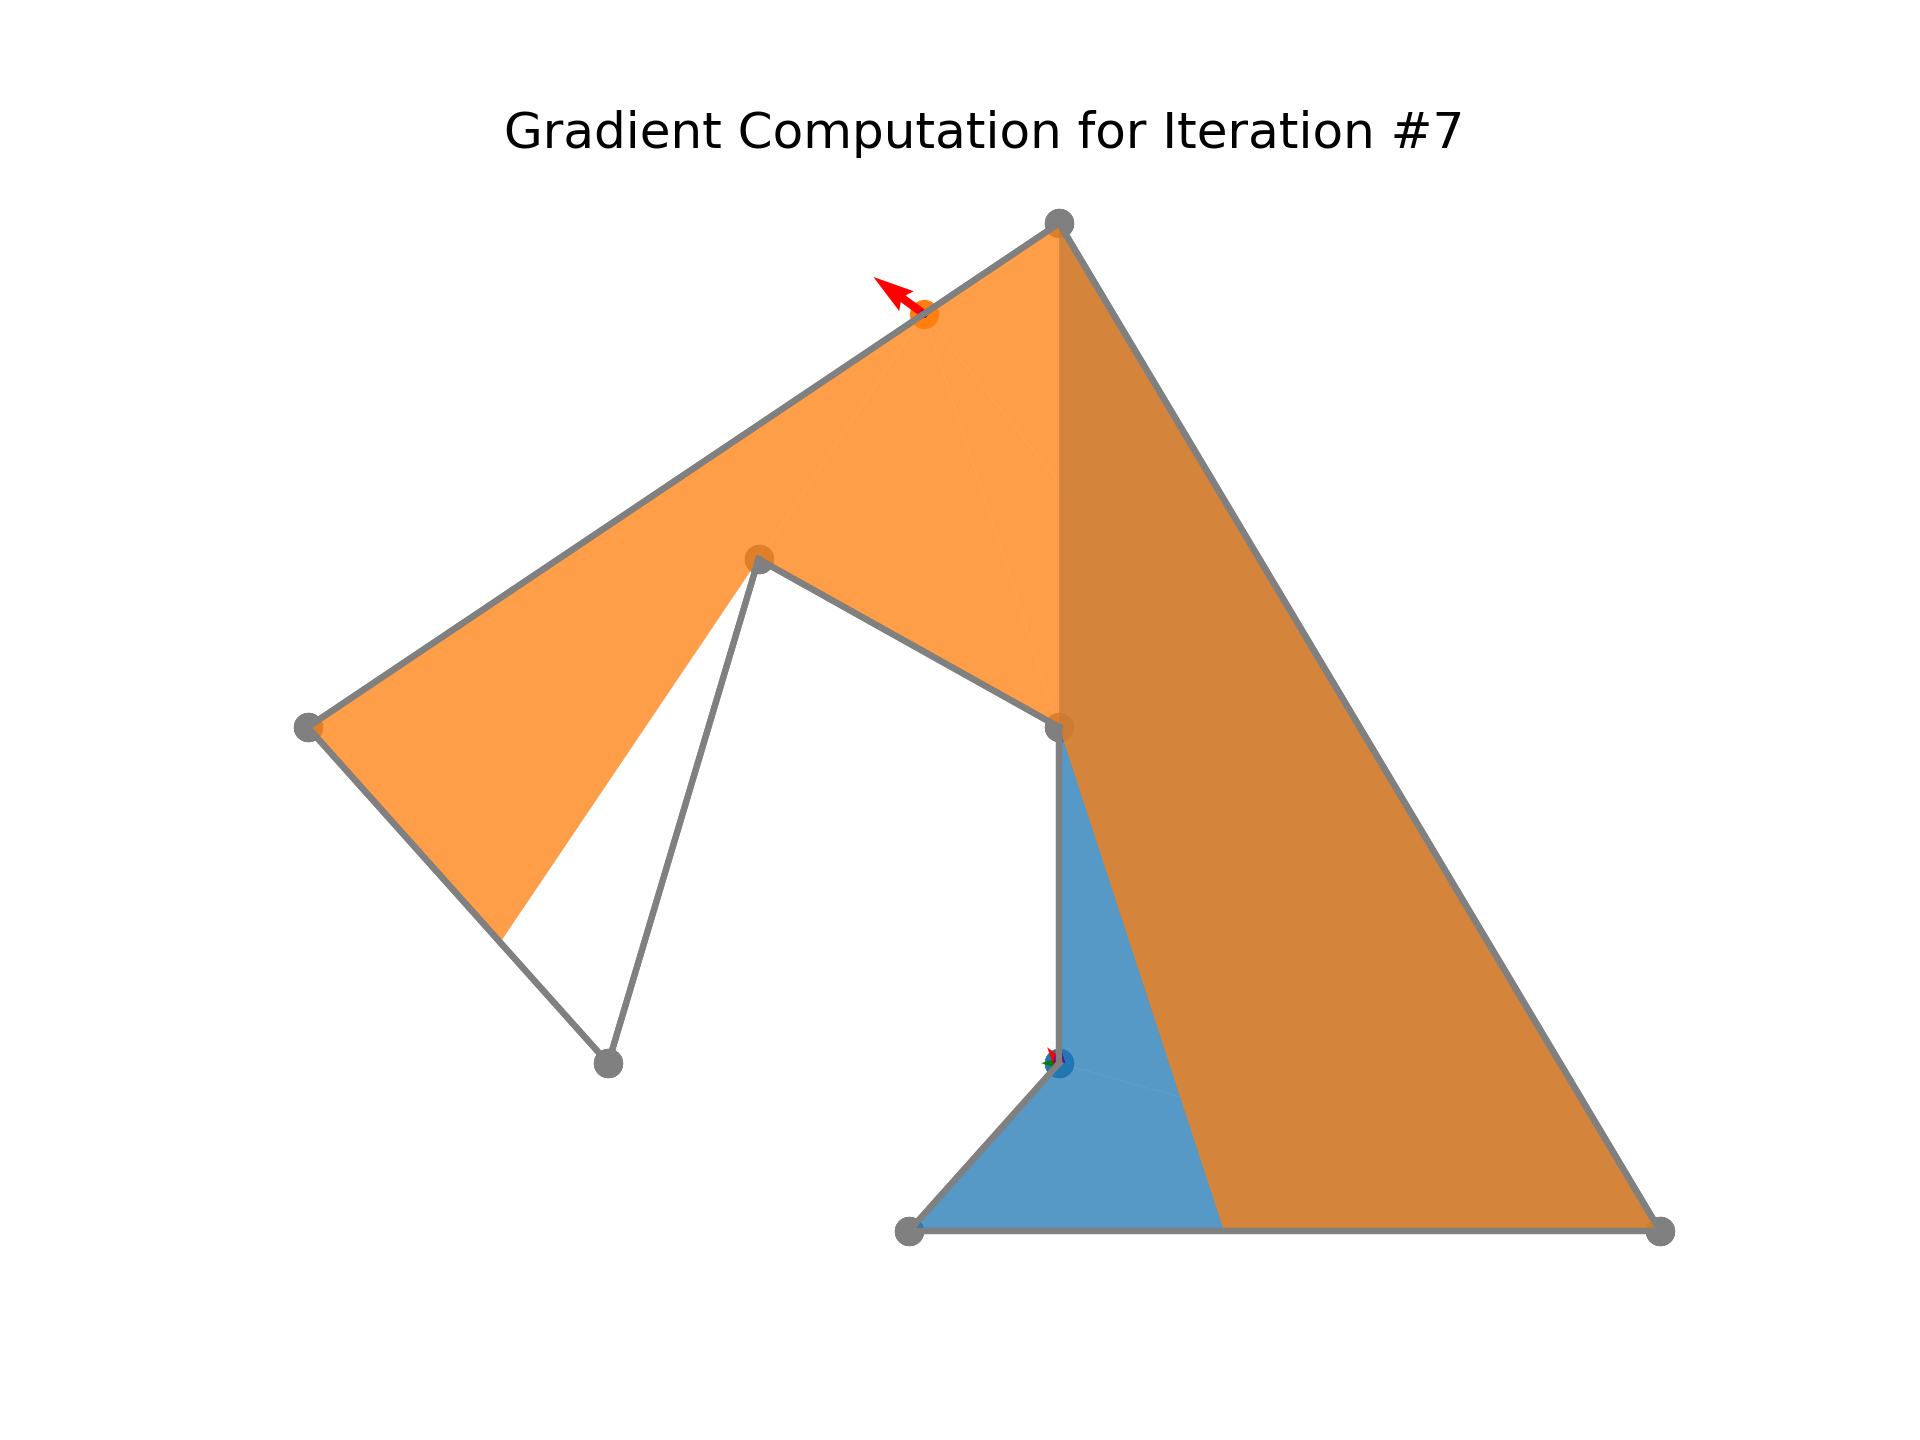
\includegraphics[width = \textwidth]{experiments/reflex_area_no_pos7.png}
        \caption{No reflex area, iteration 7. The blue guard is back on the reflex vertex.}
        \label{fig:reflex_area_no4}
    \end{subfigure}
    \caption{Comparison between using and not using the reflex area heuristic on an arbitrary polygon.}
    \label{fig:reflex_area_eg}
\end{figure}

Figure \ref{fig:reflex_area_eg} displays the difference in the areas seen between the two approaches. When using all heuristics (Subfigure \ref{fig:area_reflex_area_all}), the algorithm terminates in 7 iteration. The continuous line clearly marks the guard who did not move away from the reflex vertex. When not using the reflex area heuristic (Subfigure \ref{fig:area_reflex_area_no}), the algorithm appears not to terminate. One of the guards loops away and back on the reflex vertex. The other guard loops so that it sees the area that is being seen and unseen by the other guard. In this way, they do not synchronise in order to see the polygon together at the same time.

\begin{figure}[h!]
    \centering
    \begin{subfigure}{0.45\textwidth}
        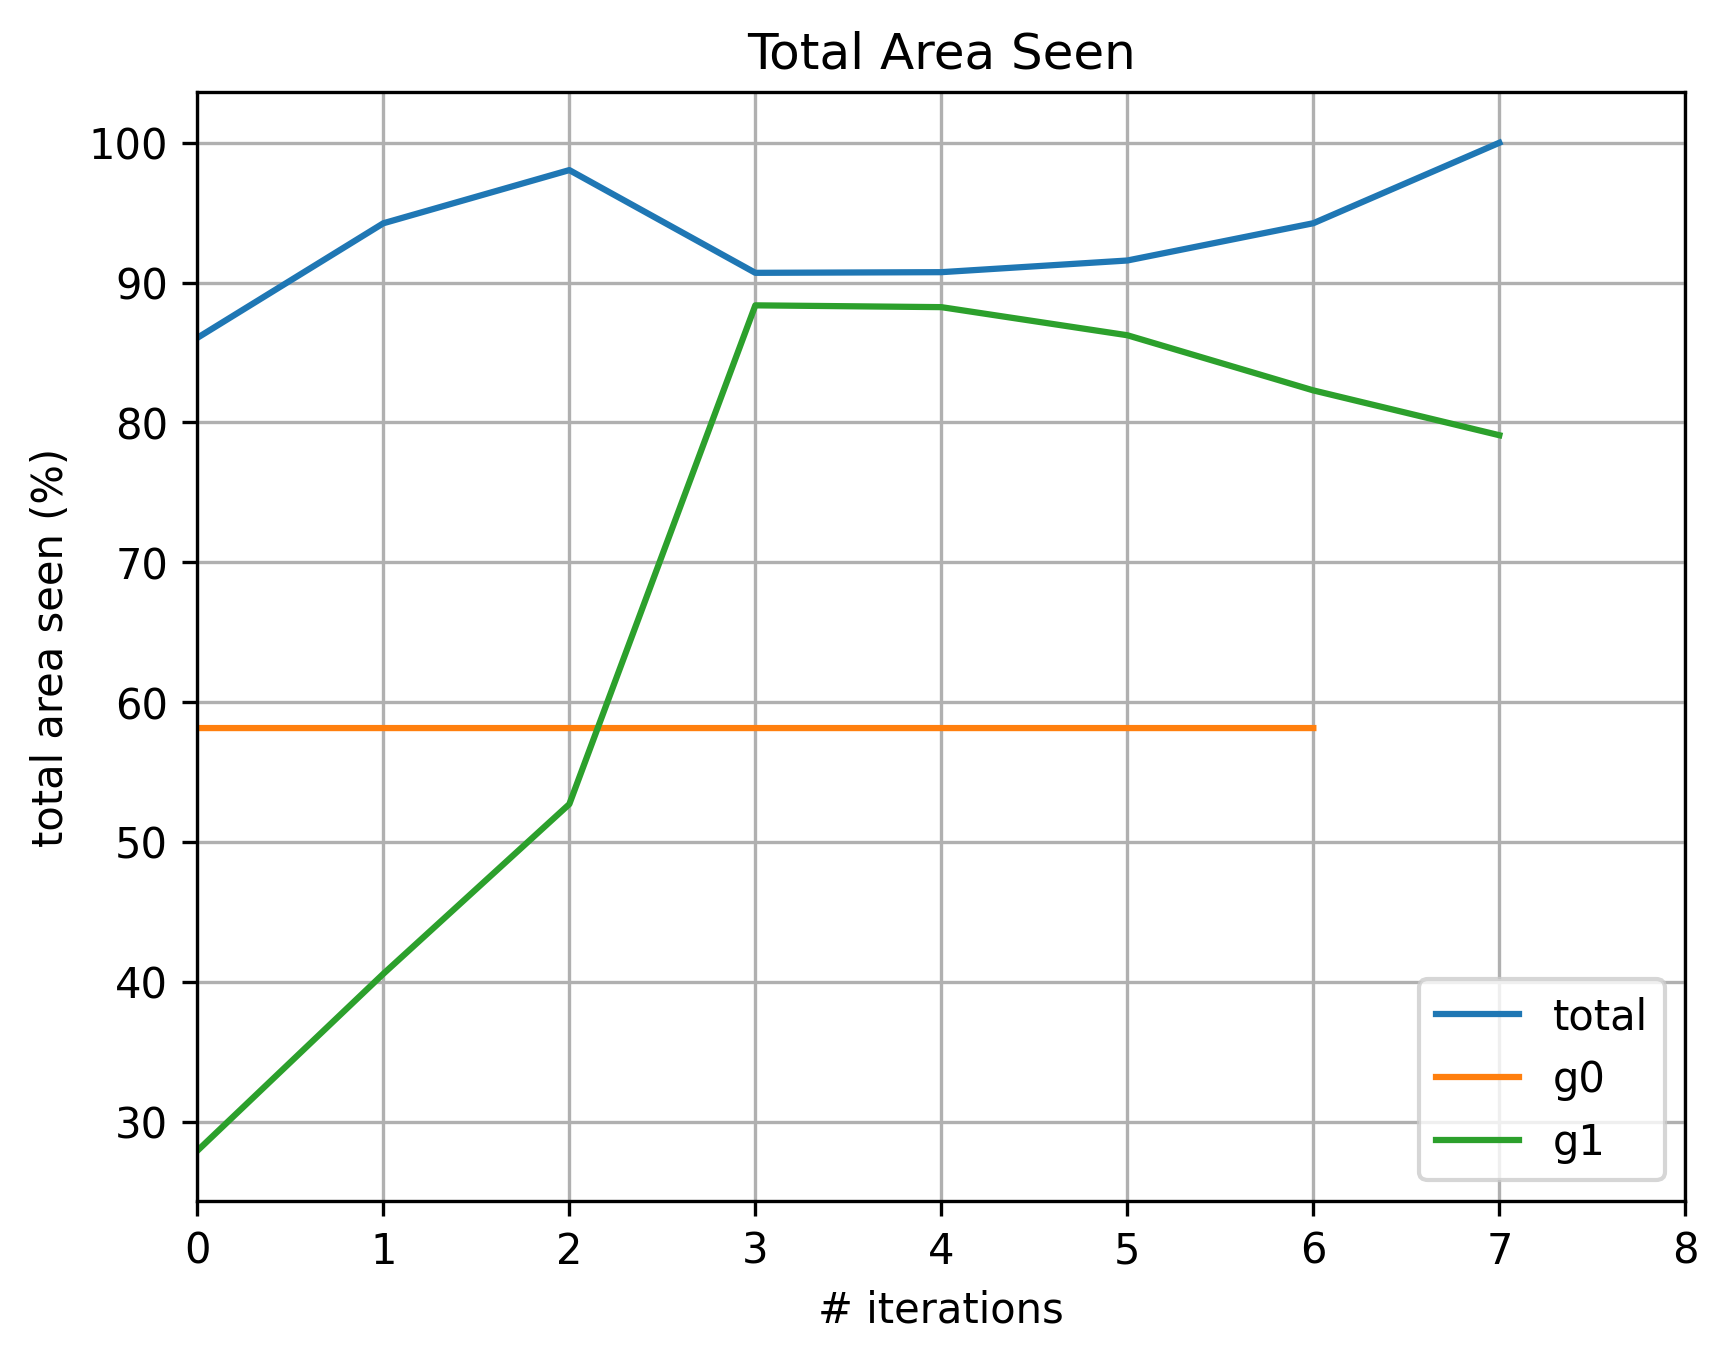
\includegraphics[width = \textwidth]{experiments/area_reflex_area_all.png}
        \caption{Area seen for all heuristics on another arbitrary polygon.}
        \label{fig:area_reflex_area_all}
    \end{subfigure}
    \hfill
    \begin{subfigure}{0.45\textwidth}
        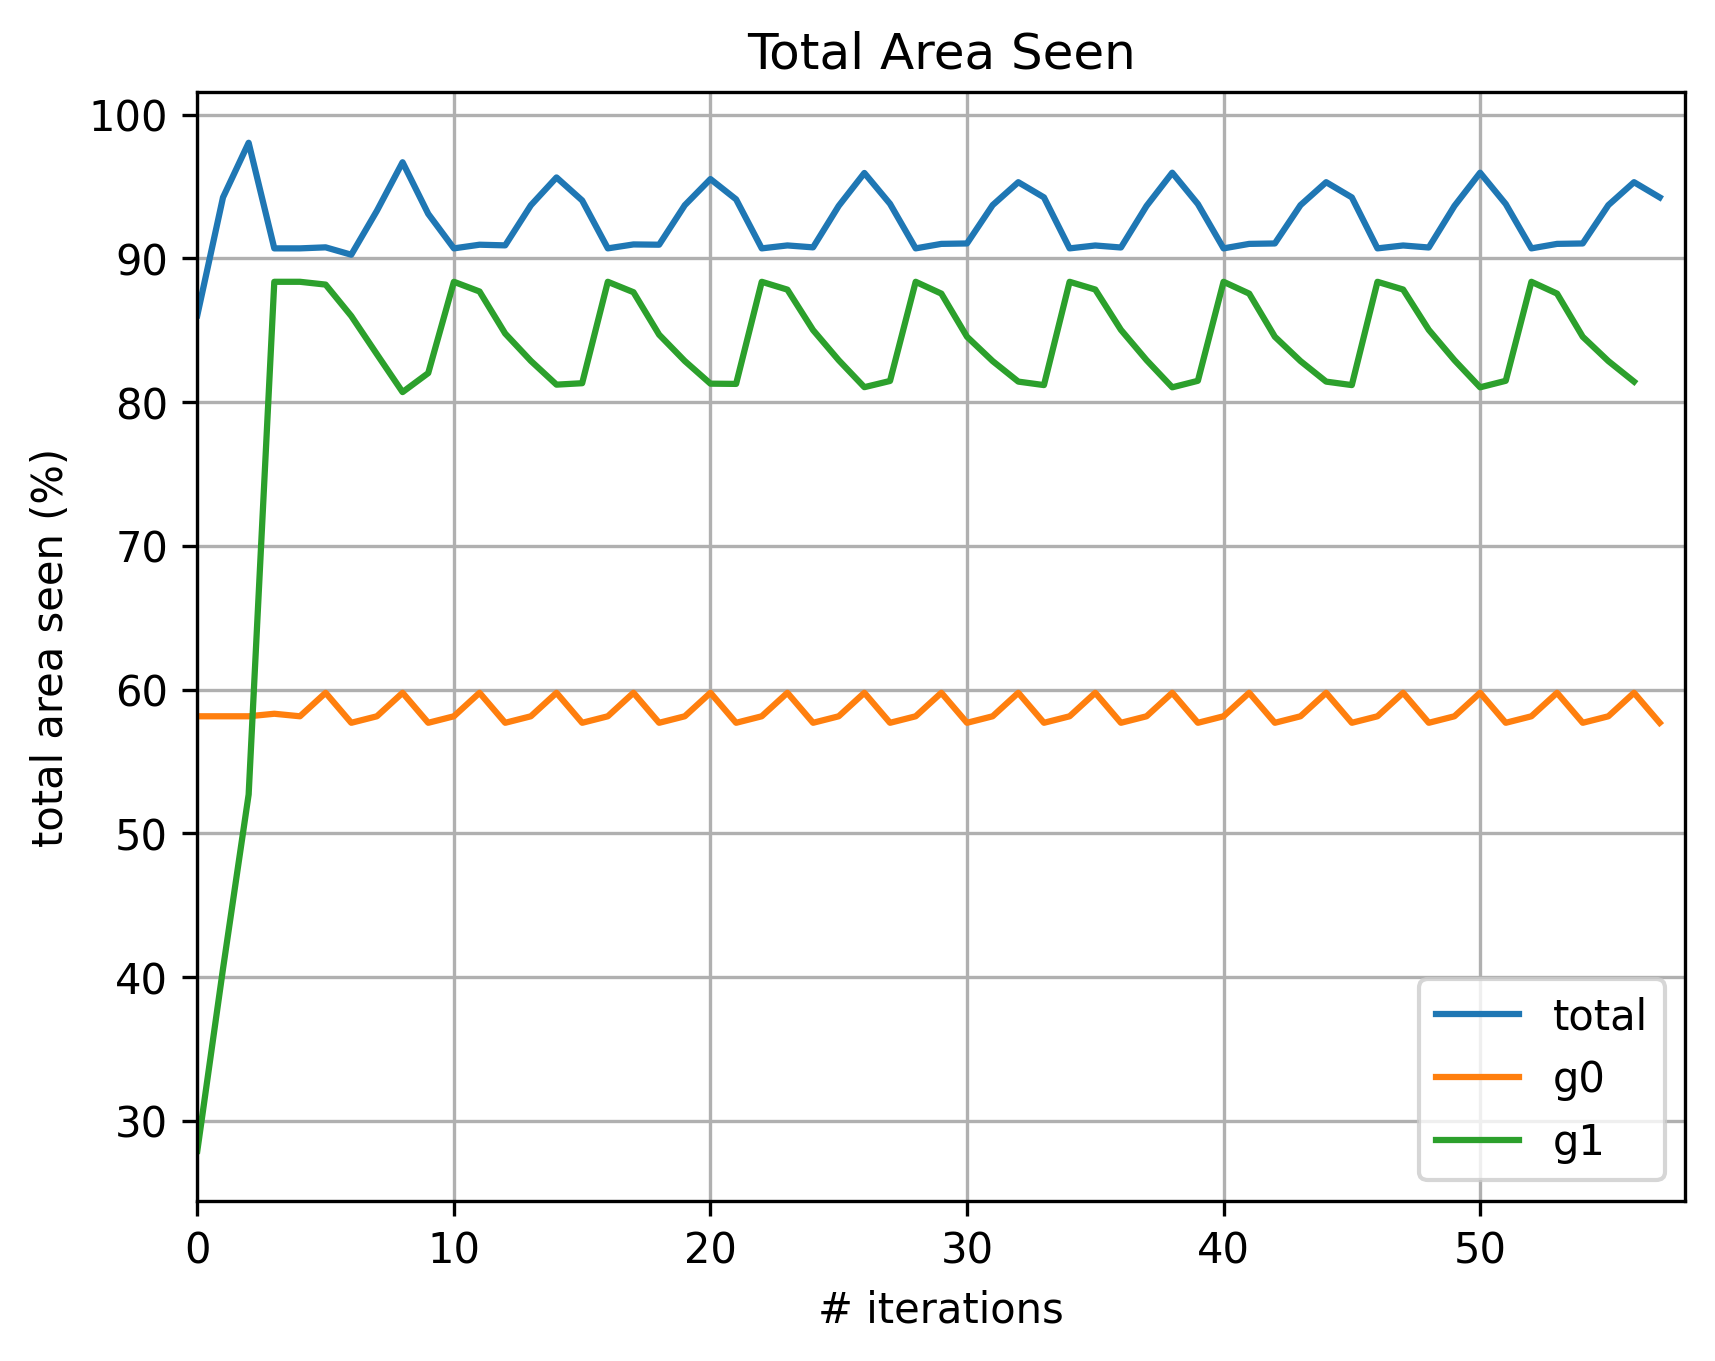
\includegraphics[width = \textwidth]{experiments/area_reflex_area_no.png}
        \caption{Area seen for no reflex area heuristic on another arbitrary polygon.}
        \label{fig:area_reflex_area_no}
    \end{subfigure}
    \caption{Area comparison between using and not using the reflex area heuristic on an arbitrary polygon.}
    \label{fig:area_reflex_area}
\end{figure}

Therefore, we believe that the reflex area heuristic is of great importance to the correct run of the algorithm. It addresses the issue of guards moving away and back on reflex vertices. This behaviour causes the other guards to move towards the area that becomes unseen by the first guard. In this way, the guards continue to move out of sync with each other, resulting in the polygon never being fully seen.

\subsubsection{No Hidden Gradient}
In this section we will discuss the importance of using a hidden gradient heuristic. Section \ref{sec:hidden_gradient} introduced this heuristic. The idea is based on the fact that we want guards to make progress, no matter how little. If a guard's visibility region is already seen by other guards, it is unlikely that its position is optimal. Thus, we want the guard to still move.

We will compare how the guards move when we are using all the heuristics to when we are not moving guards when their visibility region is fully seen by other guards. We will use the comb polygon with four teeth as an example. 

Figure \ref{fig:area_no_hidden_gradient} displays a comparison between using and not using hidden gradient in our algorithm. In Subfigure \ref{fig:area_comb_no_hidden_gradient} we can notice that the execution of the algorithm takes twice as many iterations than in Subfigure \ref{fig:area_comb_all2}. The reason behind this is the fact that for half of the iterations two of the guards do not move when no hidden gradient is used. Additionally, the total area seen in that case fluctuates. This is in contrast with the case where the hidden gradient heuristic is used. In that case, the total area seen is continuously increasing, and all guards who can make progress move.

Therefore, we believe that the hidden gradient heuristic results in a significant improvement to our algorithm in terms of efficiency. In this way, all guards are ensured to make some progress towards their optimum and are not stalled.

\begin{figure}[h!]
    \centering
    \begin{subfigure}{0.45\textwidth}
        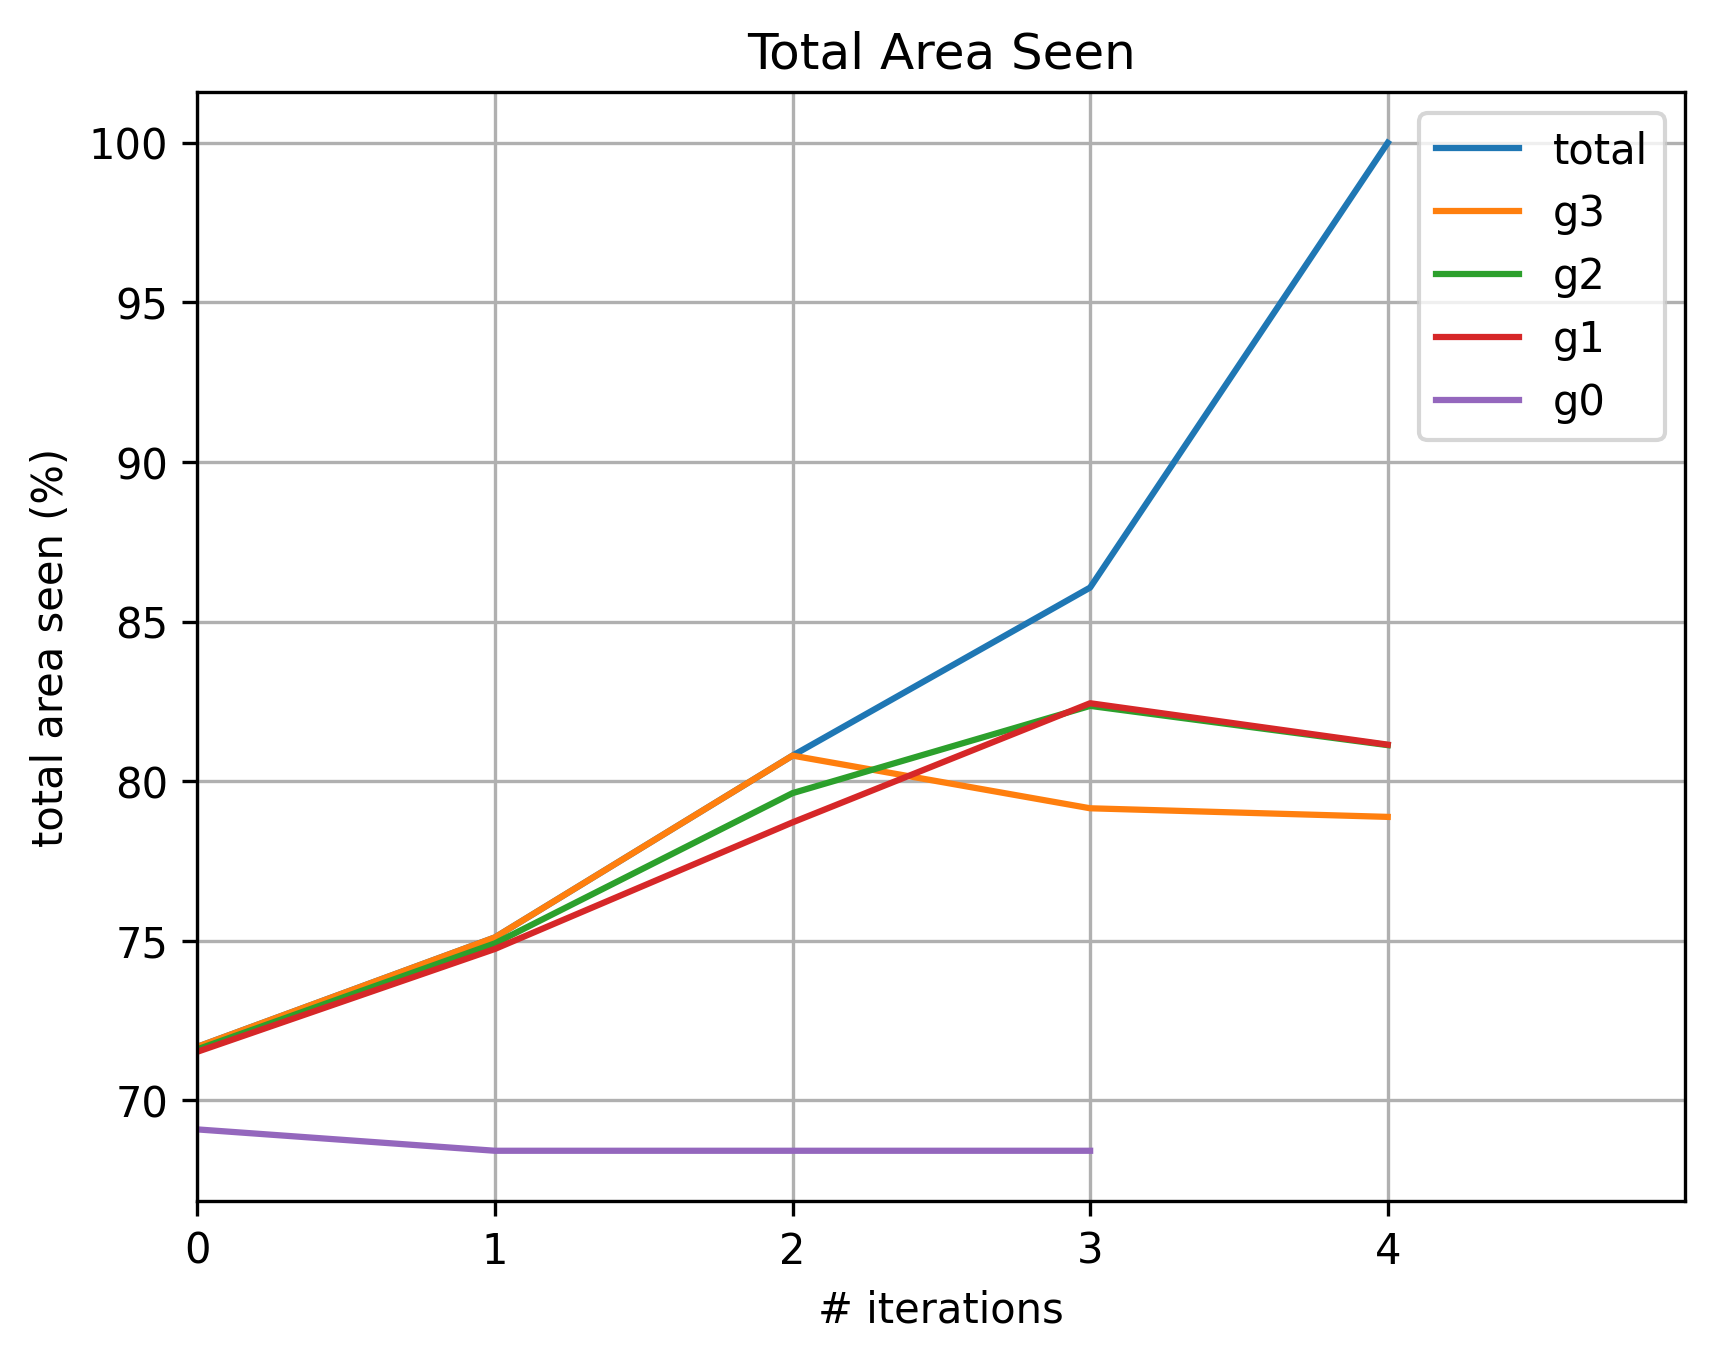
\includegraphics[width = \textwidth]{experiments/area_comb_all.png}
        \caption{All heuristics.}
        \label{fig:area_comb_all2}
    \end{subfigure}
    \begin{subfigure}{0.45\textwidth}
        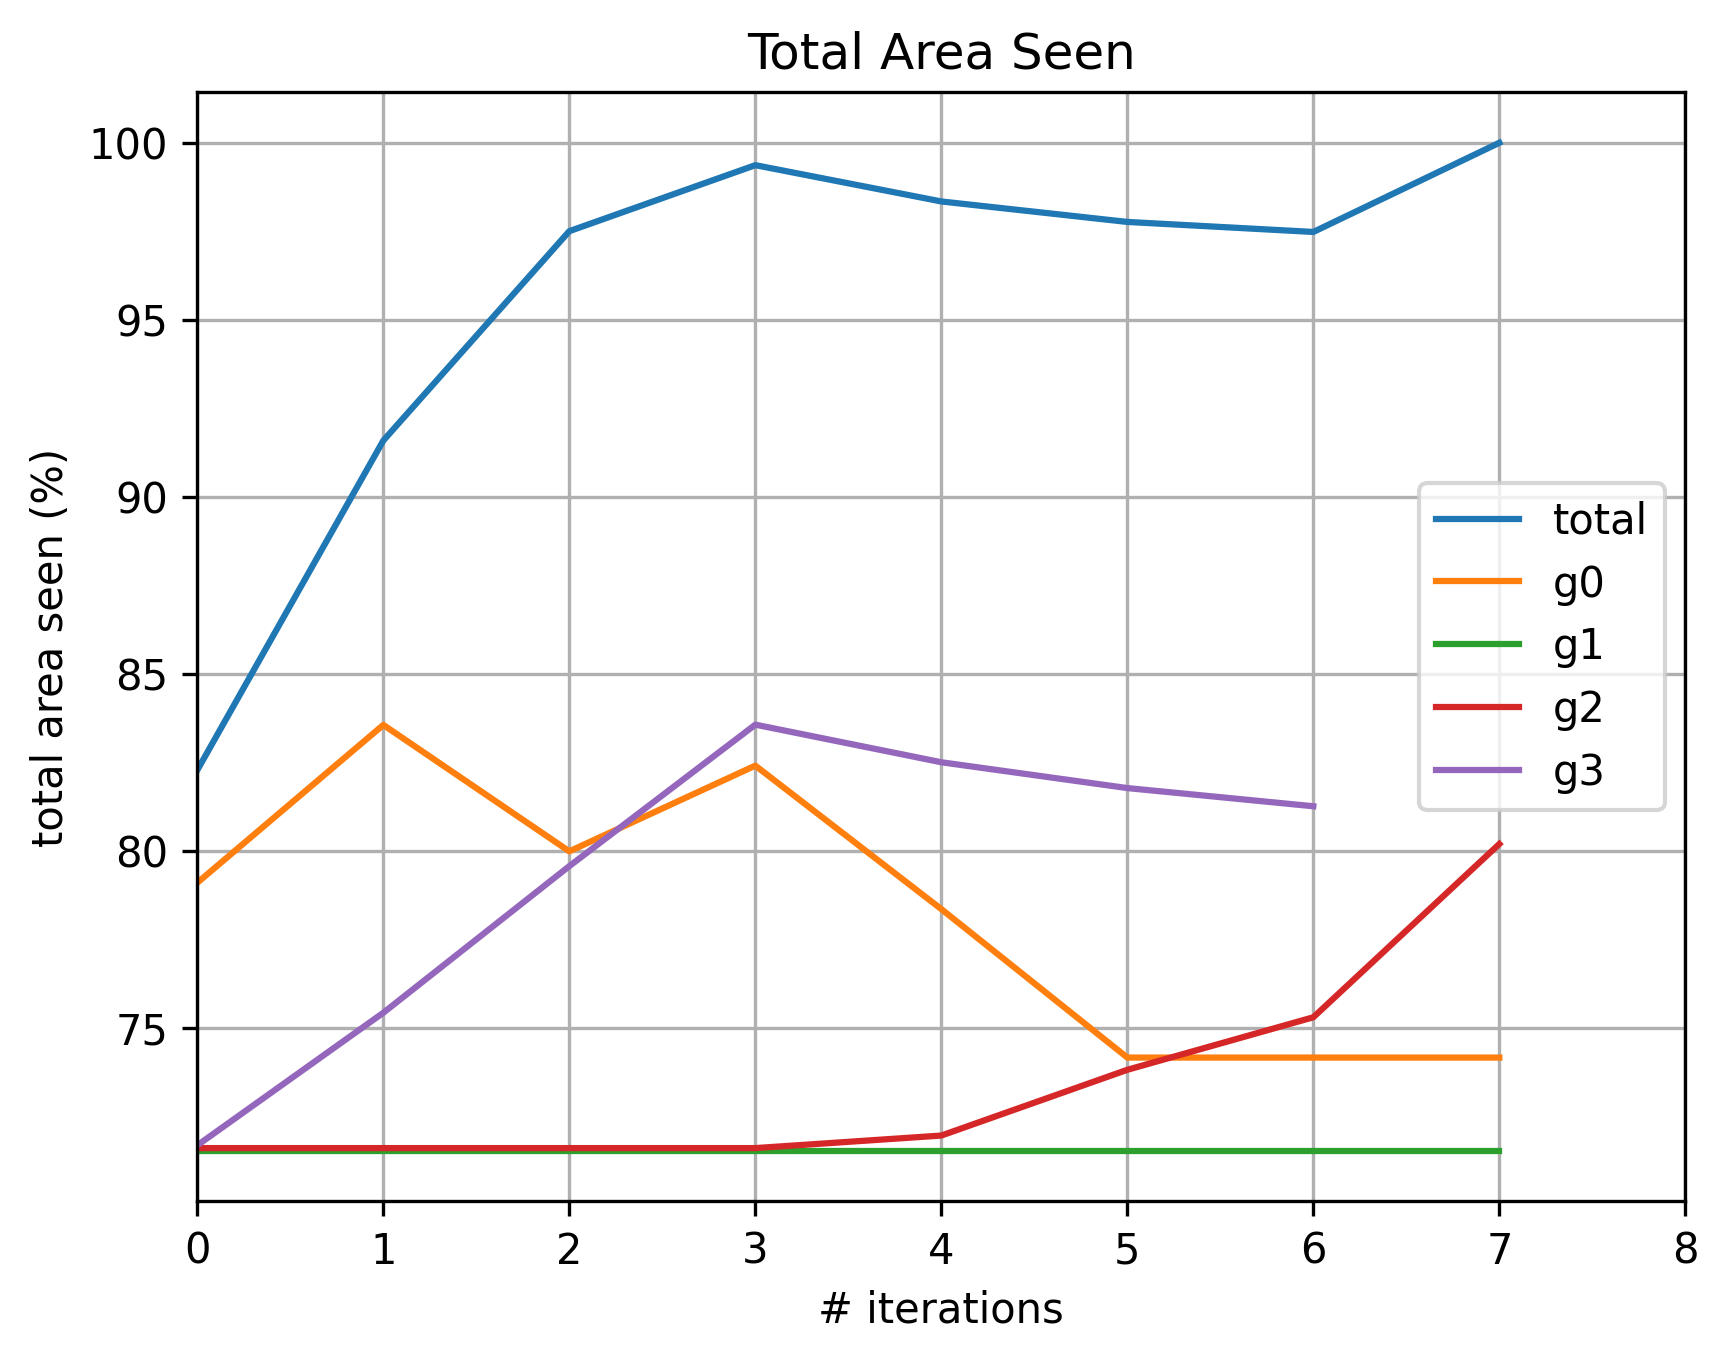
\includegraphics[width = \textwidth]{experiments/area_comb_no_hidden_gradient.png}
        \caption{No hidden gradient.}
        \label{fig:area_comb_no_hidden_gradient}
    \end{subfigure}
    \caption{Seen area for the comb polygon with four teeth.}
    \label{fig:area_no_hidden_gradient}
\end{figure}

\subsubsection{Without Angle Behind Reflex Vertex}
In this section we will discuss the benefits of using the value of the angle behind reflex vertices. Section \ref{sec:angle} introduced this heuristic. The idea behind this technique is that guards should be drawn faster to larger unseen areas behind reflex vertices. Conversely, if the unseen area behind the reflex vertex is very small, we also want guards to move towards it. In this way, we prioritise unseen areas based on their size, while still accounting for the very small unseen areas.

Figure \ref{fig:no_angle} shows a comparison between using and not using the angle behind the reflex vertex heuristic: Subfigures \ref{fig:all_angle_pos0} and \ref{fig:all_angle_pos1} display the first two iterations of the algorithm when all heuristics are used, whereas  Subfigures \ref{fig:no_angle_pos0} and \ref{fig:no_angle_pos1} focus on the first two iterations when not using the angle behind the reflex vertex.
We can observe a major difference in the way the final momentum movement is computed for the orange guard in the two cases. When all heuristics are used, the movements of the guards are much smaller and calculated than when the angle does not play a role. For example, in Subfigure \ref{fig:no_angle_pos0}, the orange guard has a very large momentum movement outside of the polygon due to the unseen part in the upper pocket. When we also take into account the angles behind the reflex vertices in the pocket, its movements become much smaller (Subfigure \ref{fig:all_angle_pos0}). In fact, the orange guard is also drawn slightly the right part of the polygon, as it has a larger angle behind the reflex vertex. That part of the polygon is already seen by the blue guard, so it starts moving towards the upper pocket in Subfigure \ref{fig:all_angle_pos1}.

In terms of efficiency, the optimal solution is achieved in more iterations when the movements of the guards when the angle heuristic is used. This can be observed in Subfigures \ref{fig:area_all_angle} and \ref{fig:area_no_angle}. When using all heuristics, the random polygon is fully seen in 5 iterations. The movement of the guards is smooth. Two of the guards have an increasing seen area, whereas the orange guard moves slowly towards the upper pocket of the polygon. Not using the angle heuristic allows us to achieve the same goal in only 3 iterations. As mentioned, the progress of the guards is not as smooth.

Therefore, we believe that computing the angle behind the reflex vertex is a heuristic that allows us to fine-tune and smoothen the movement of the guards. In this way, we can focus on moving fast towards the bigger unseen areas, while also not neglecting the smaller ones. We could say that this heuristic offers a trade-off between the number of iterations and path smoothness. For this reason, we believe that the performance of the algorithm is influenced by the type of polygons it is applied to: polygons with sharper, narrower turns could benefit the most from this heuristic.

\begin{figure}[h!]
    \centering
    \begin{subfigure}{0.45\textwidth}
        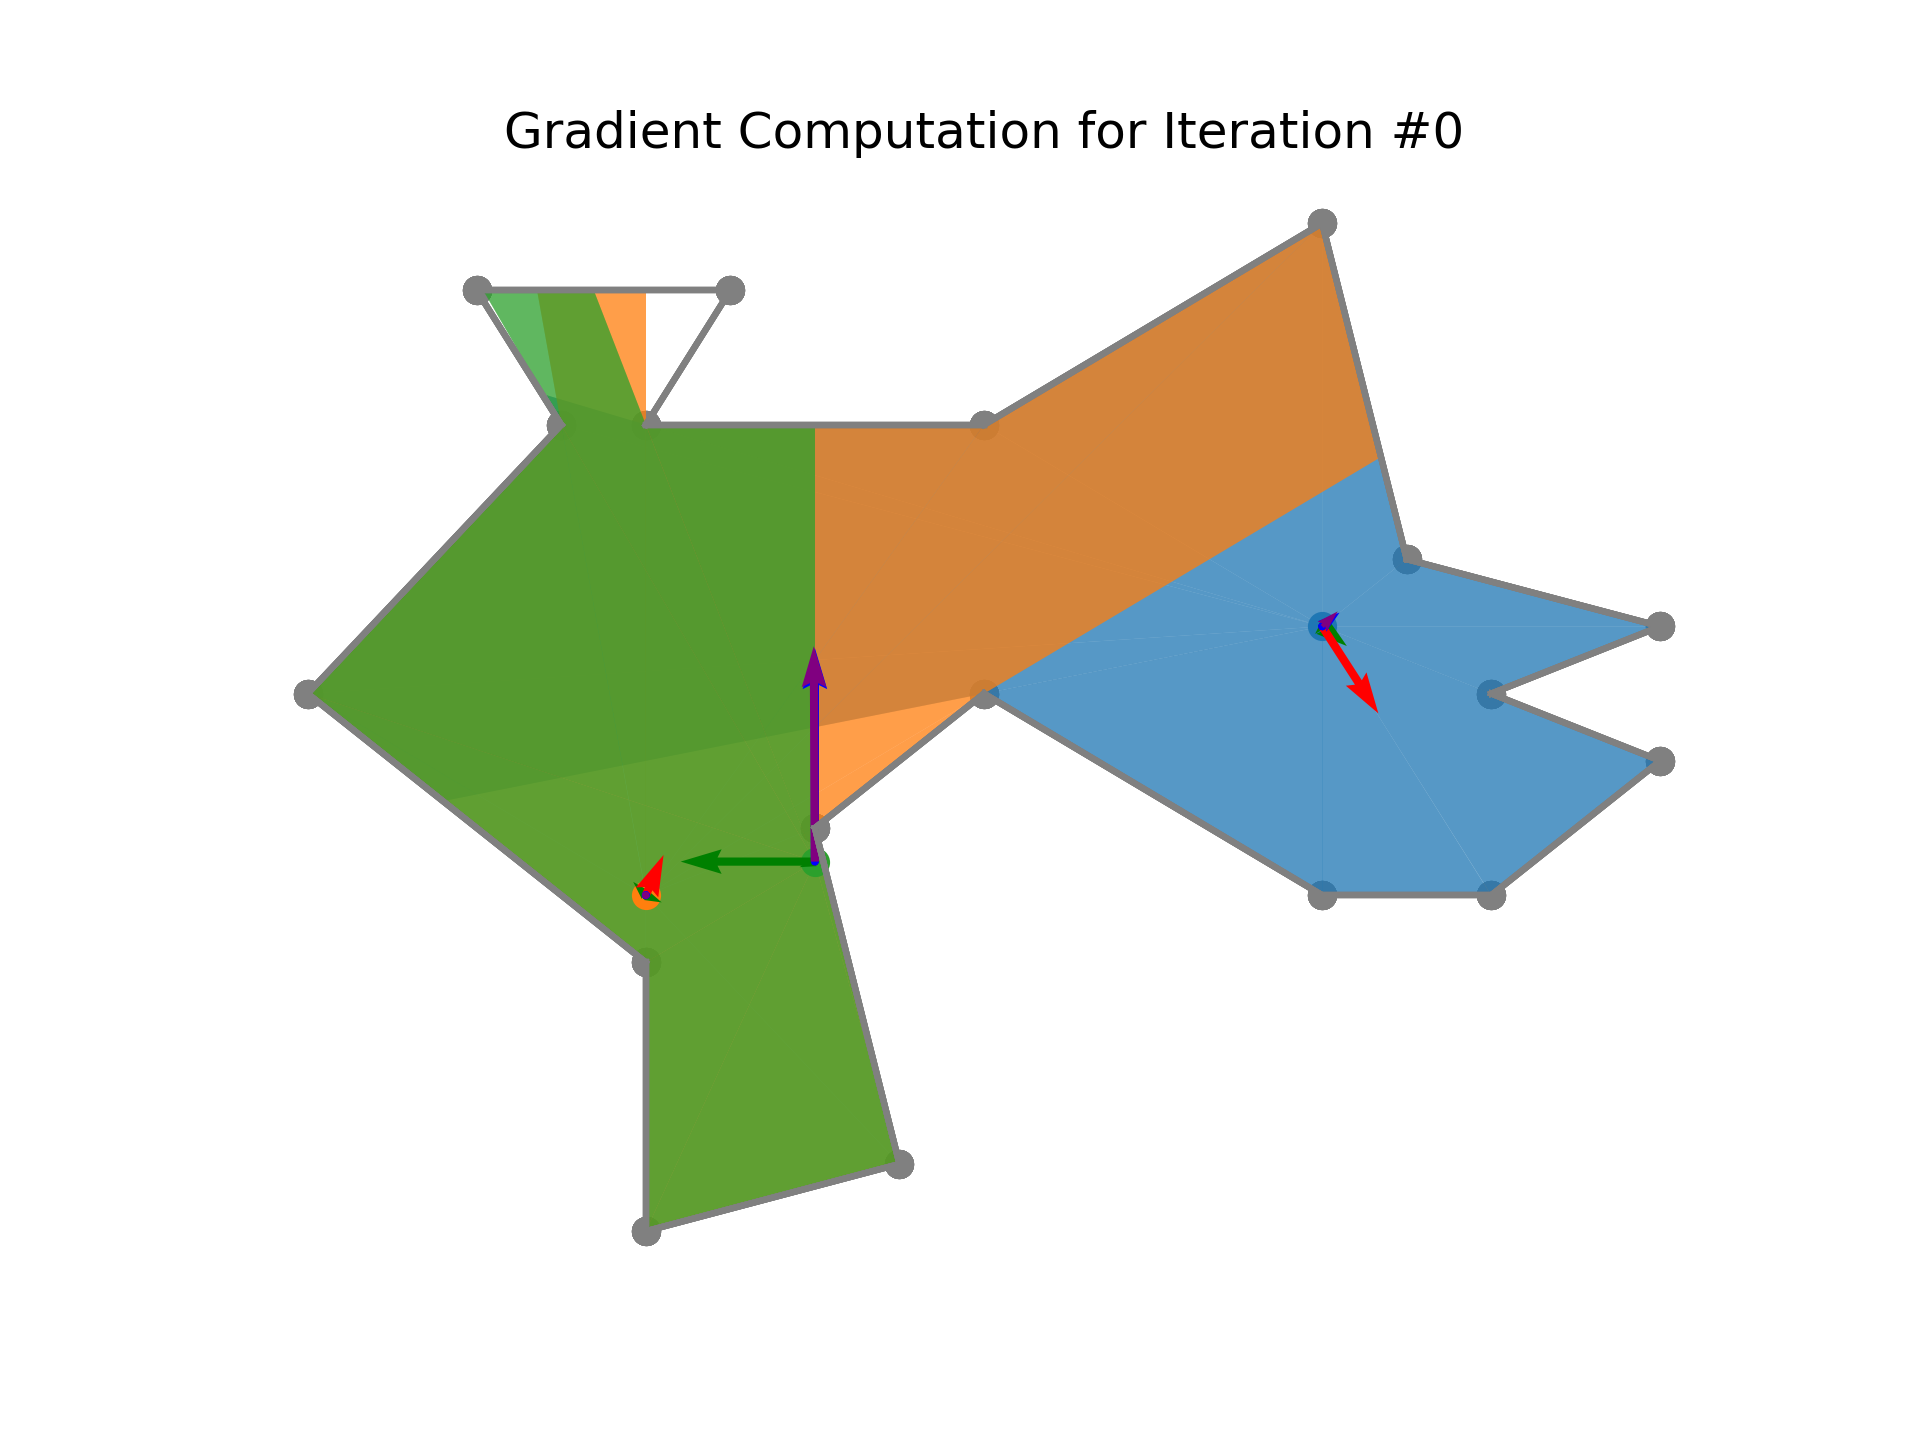
\includegraphics[width = \textwidth]{experiments/random_all_pull_pos0_fixed.png}
        \caption{All heuristics, iteration 0. The orange guard's movement is towards upper right.}
        \label{fig:all_angle_pos0}
    \end{subfigure}
    \hfill
    \begin{subfigure}{0.45\textwidth}
        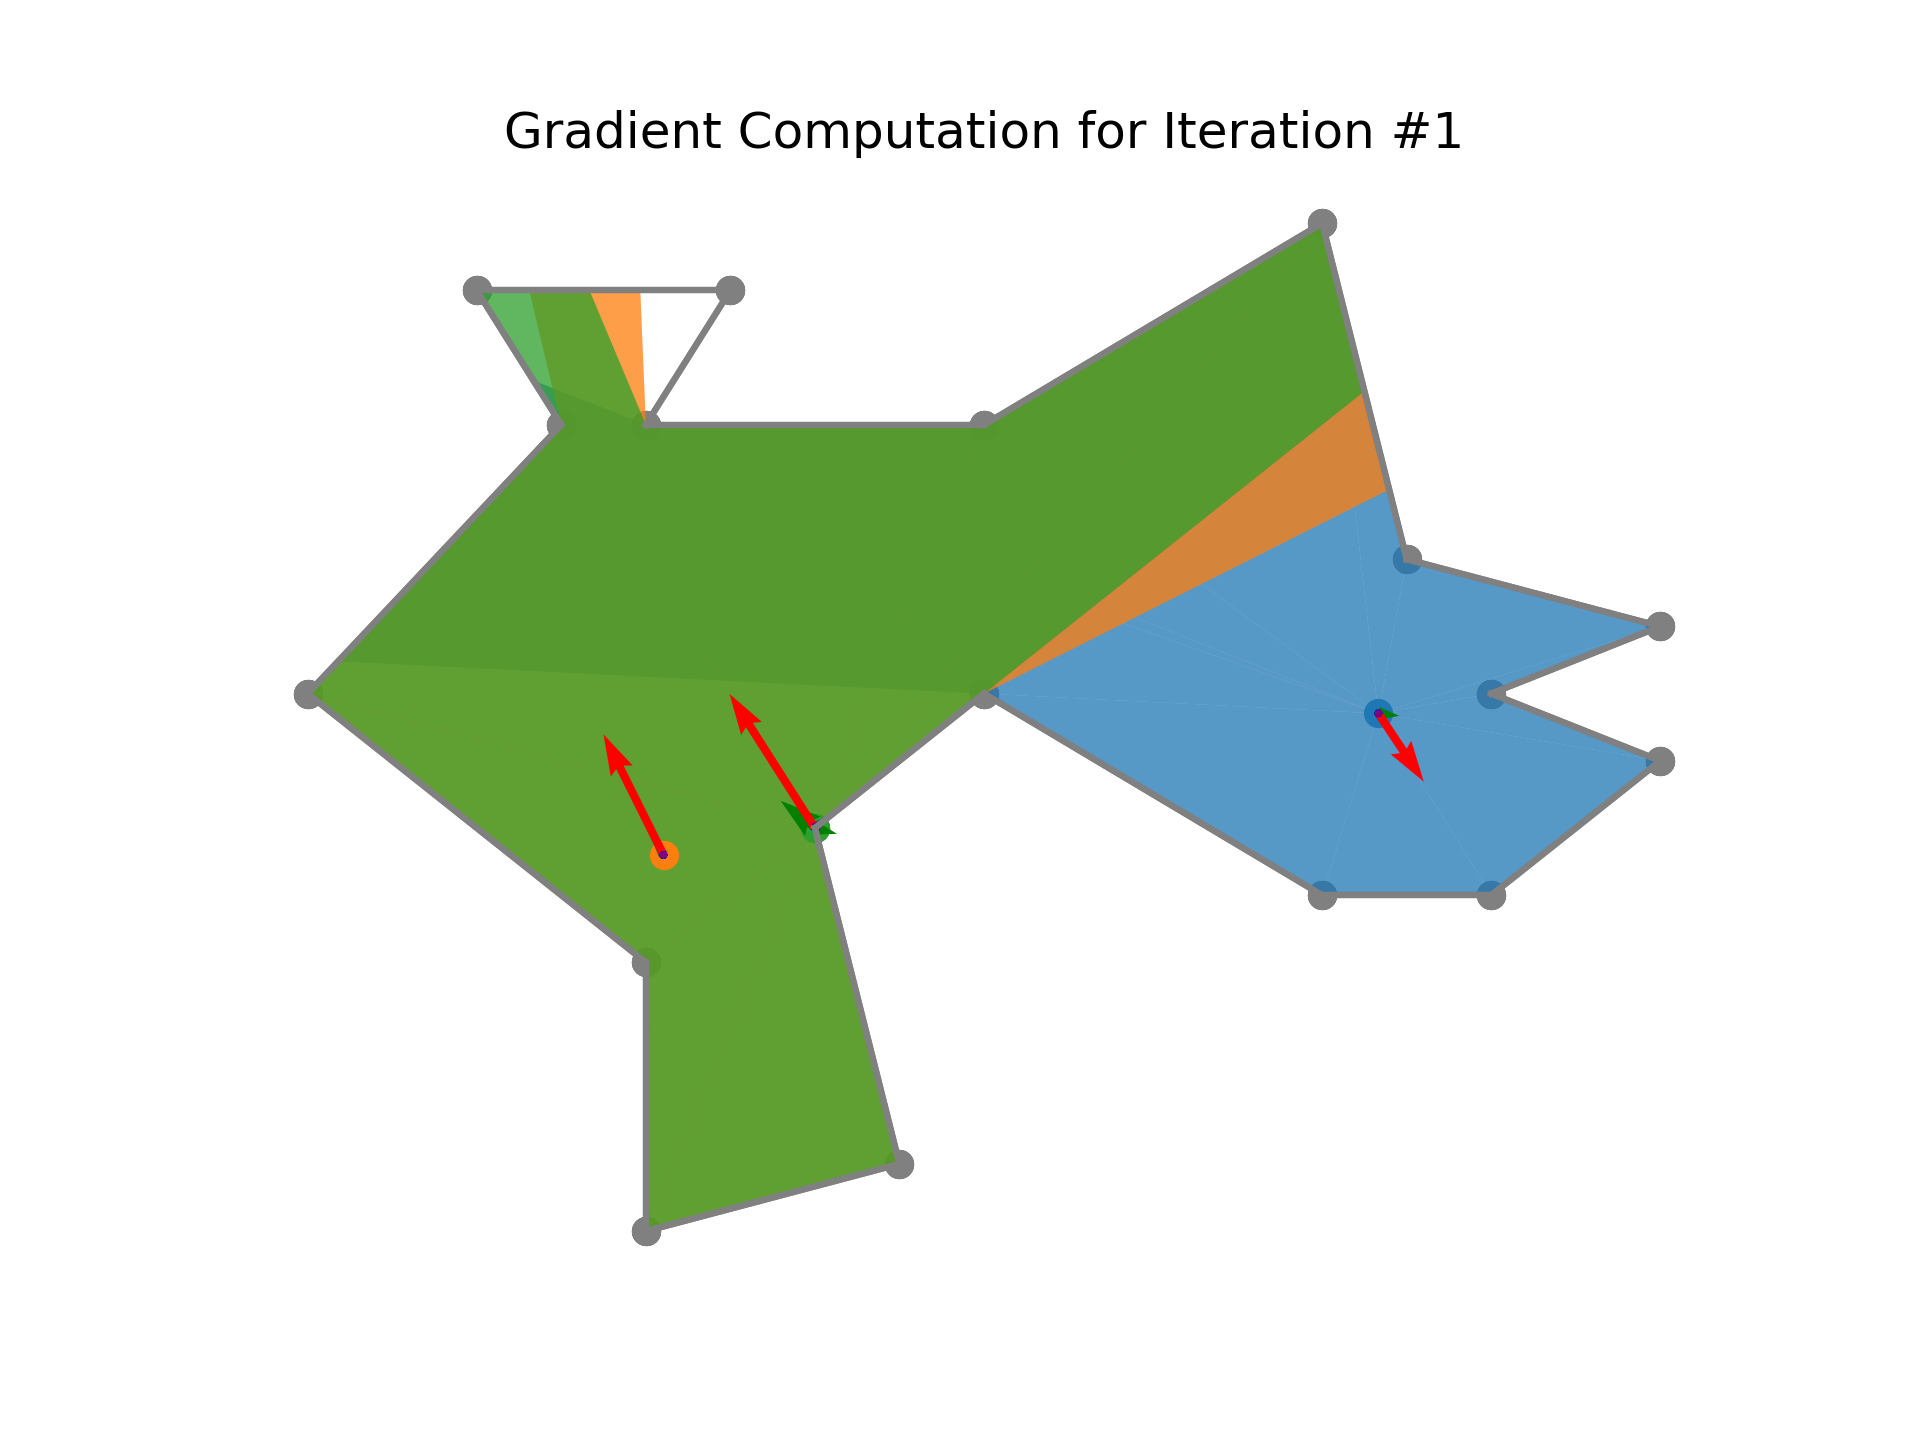
\includegraphics[width = \textwidth]{experiments/random_all_pull_pos1_fixed.png}
        \caption{All heuristics, iteration 1. The orange guard's movement is towards upper left.}
        \label{fig:all_angle_pos1}
    \end{subfigure}
    \vfill
    \begin{subfigure}{0.45\textwidth}
        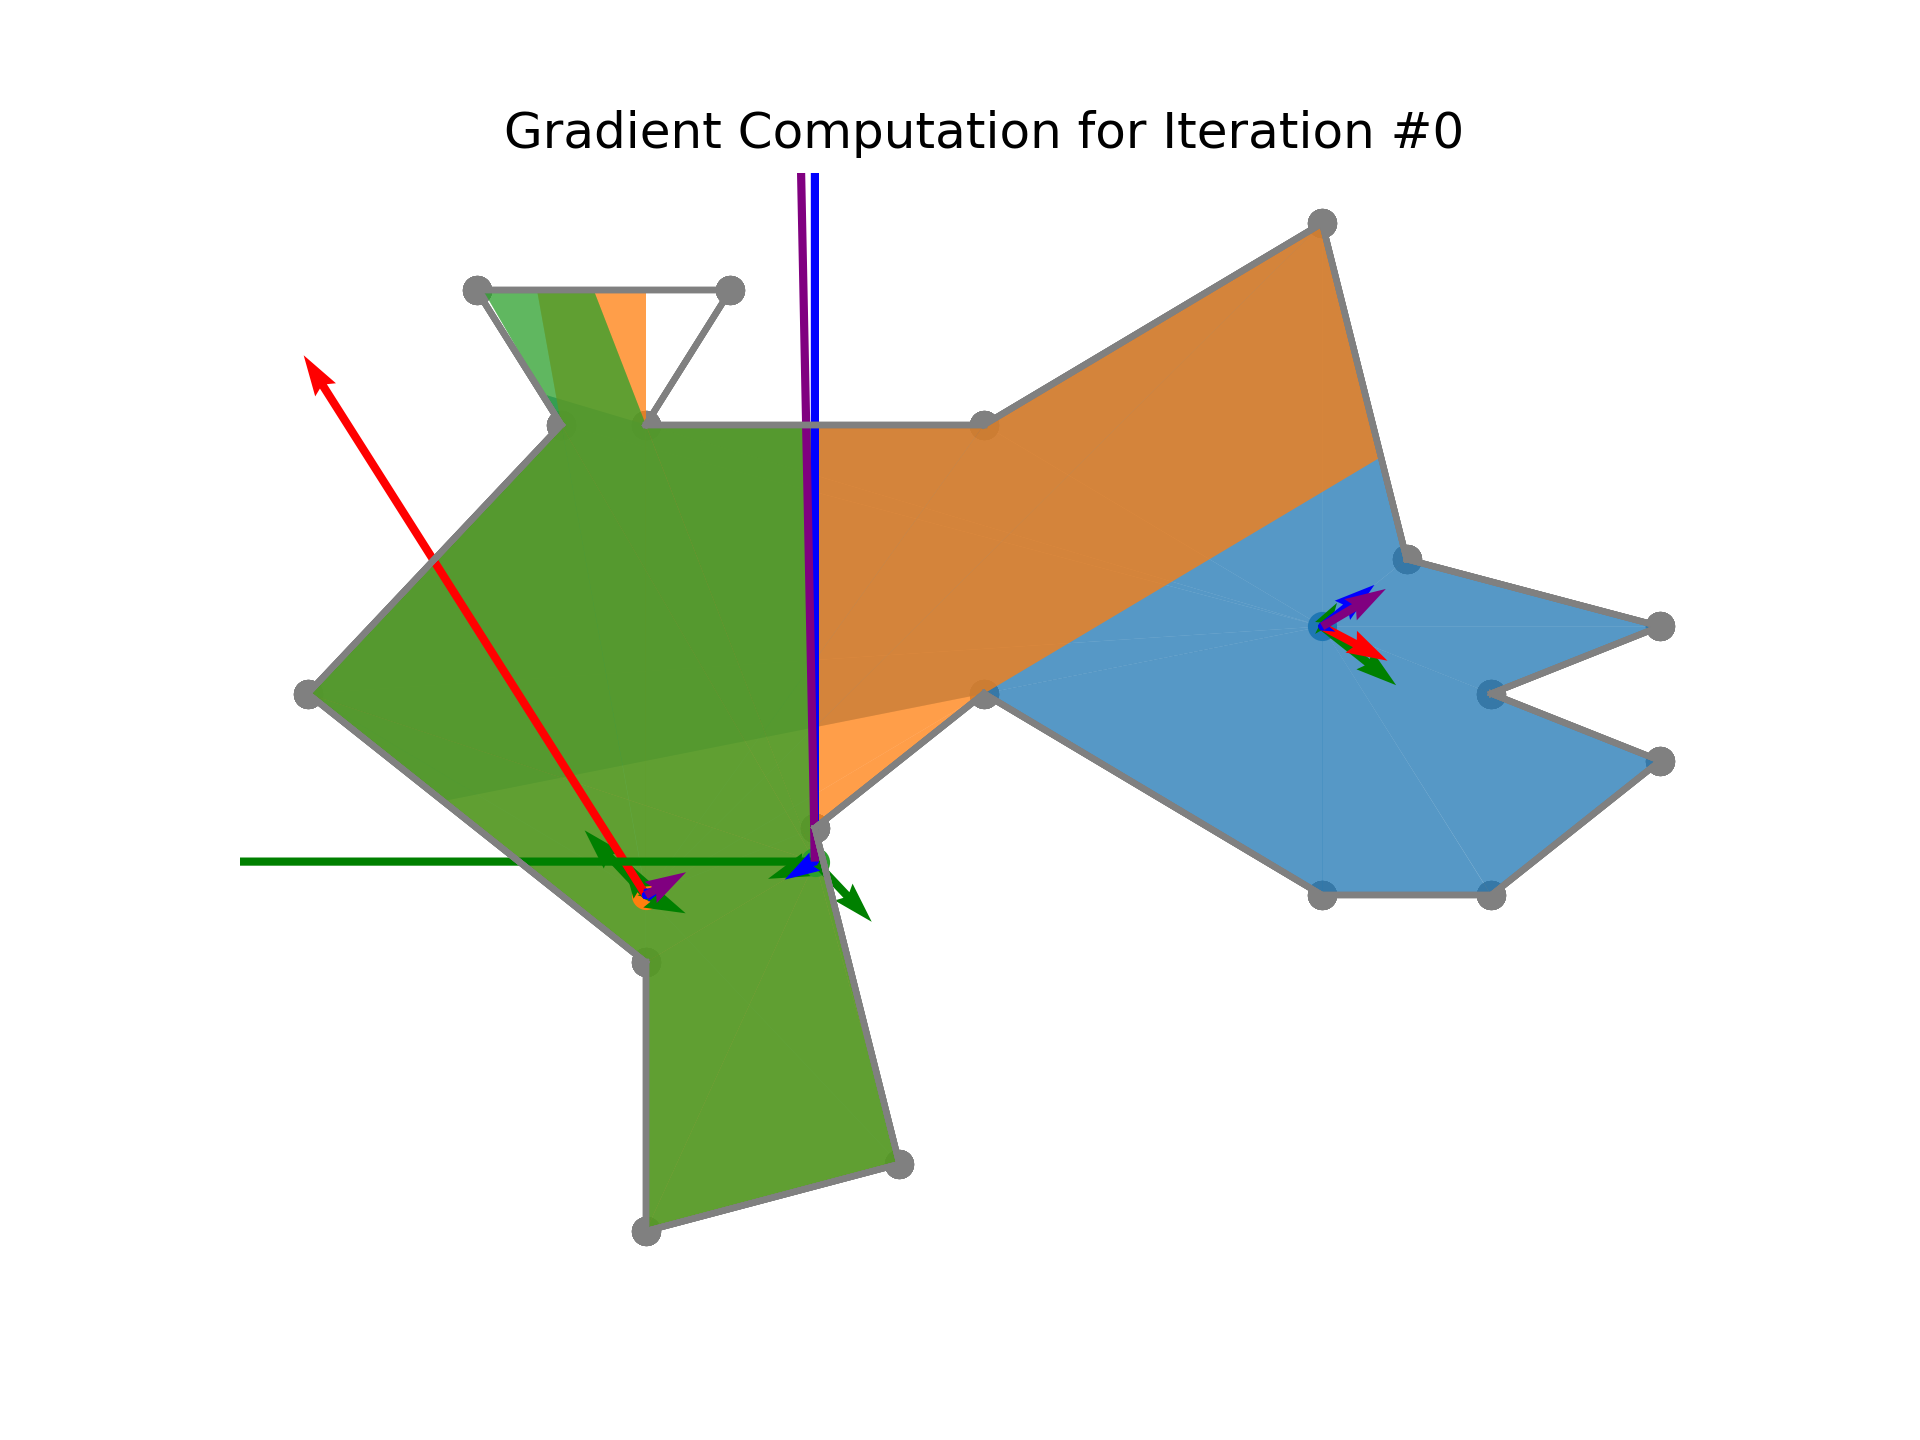
\includegraphics[width = \textwidth]{experiments/random_no_angle_pos0.png}
        \caption{No angle behind the reflex vertex, iteration 0. The orange guard's movement is all the way to the left boundary of the polygon.}
        \label{fig:no_angle_pos0}
    \end{subfigure}
    \hfill
    \begin{subfigure}{0.45\textwidth}
        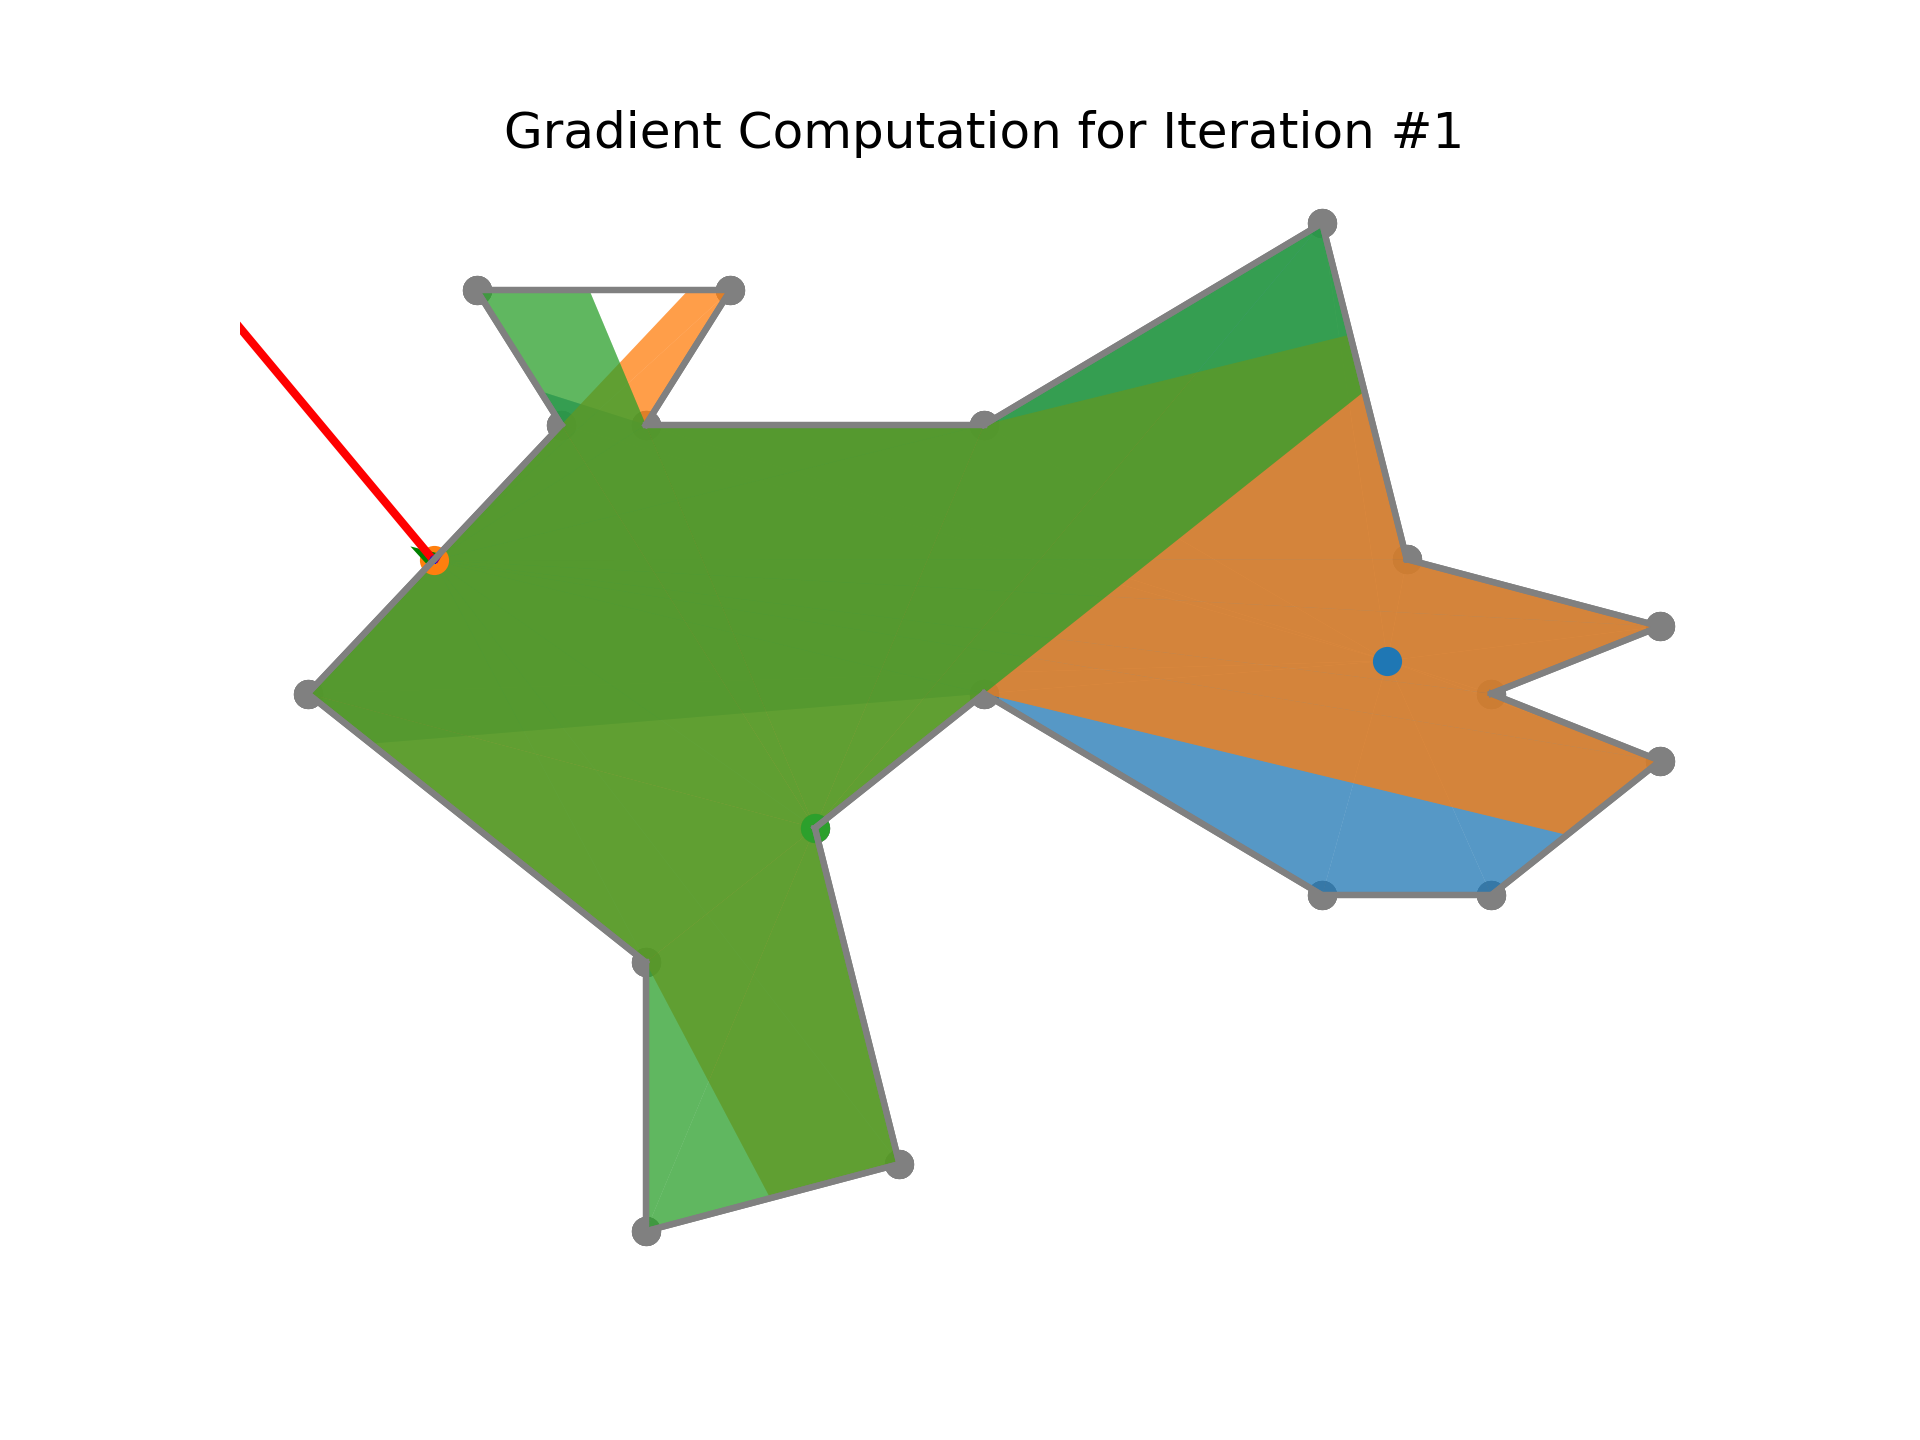
\includegraphics[width = \textwidth]{experiments/random_no_angle_pos1.png}
        \caption{No angle behind the reflex vertex, iteration 1. The orange guard's movement is towards the left-side outside of the polygon.}
        \label{fig:no_angle_pos1}
    \end{subfigure}
    \vfill
    \begin{subfigure}{0.45\textwidth}
        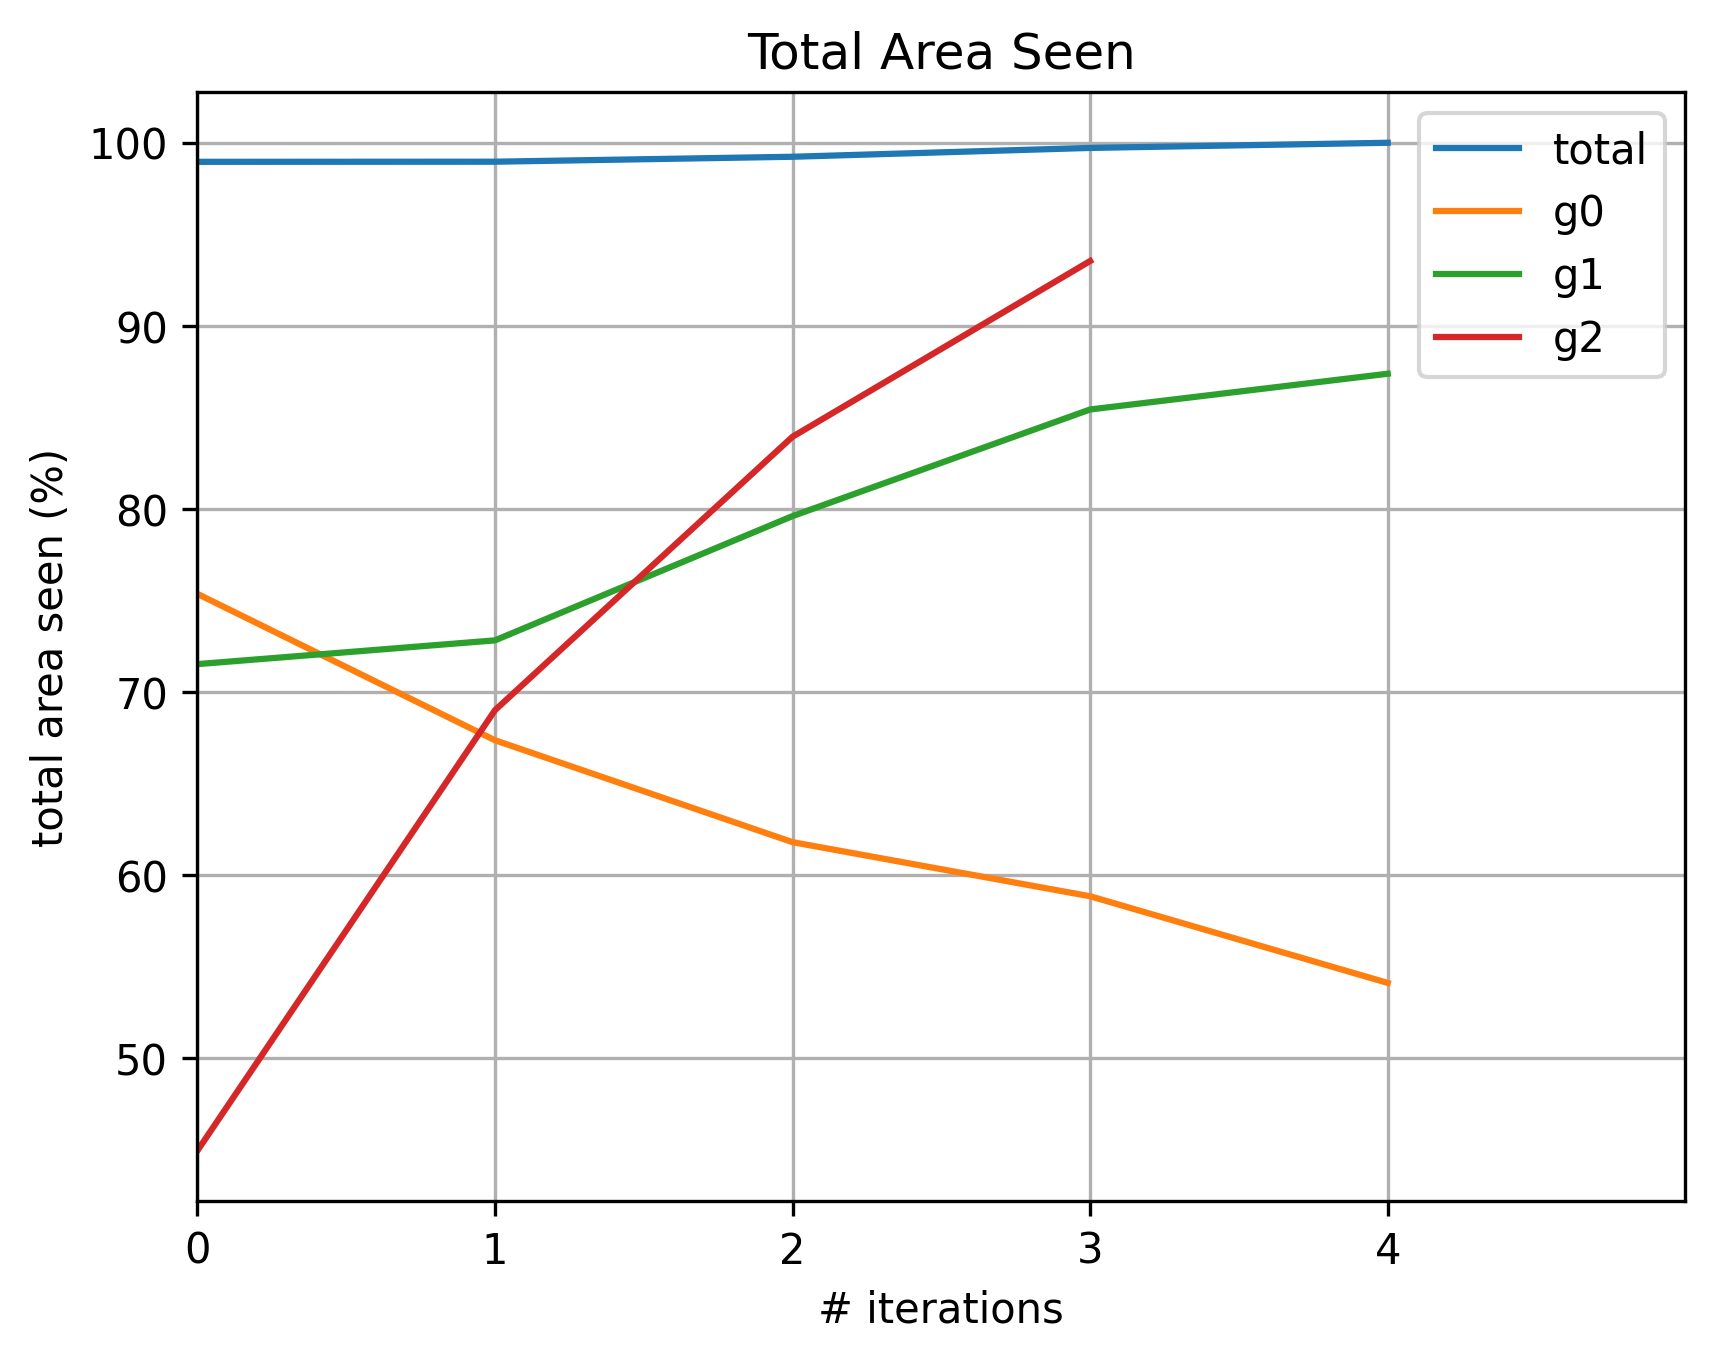
\includegraphics[width = \textwidth]{experiments/area_random_all_fixed.png}
        \caption{Seen area for all heuristics.}
        \label{fig:area_all_angle}
    \end{subfigure}
    \hfill
    \begin{subfigure}{0.45\textwidth}
        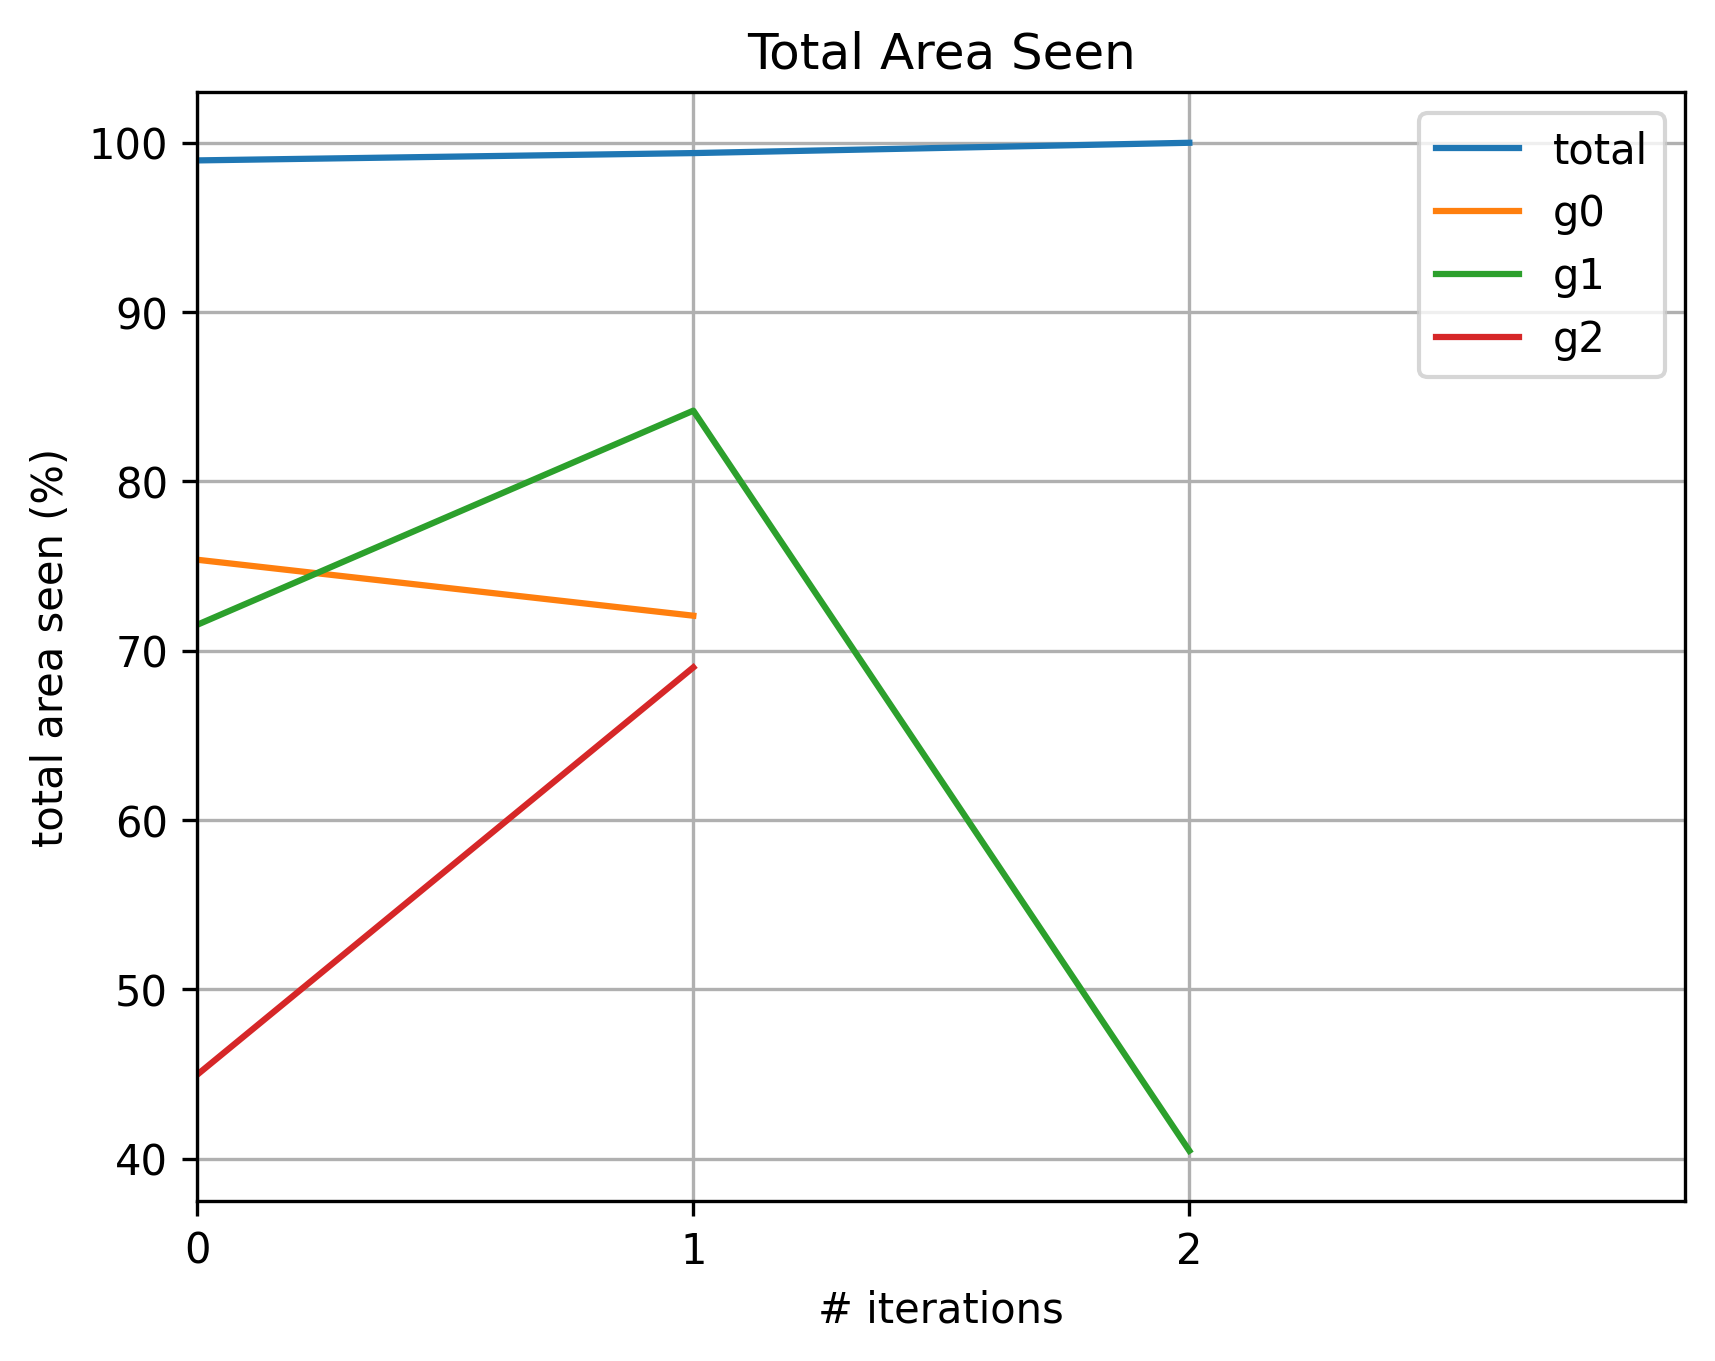
\includegraphics[width = \textwidth]{experiments/area_random_no_angle.png}
        \caption{Seen area without the angle behind the reflex vertices.}
        \label{fig:area_no_angle}
    \end{subfigure}
    \caption{Comparison between using and not using the angle behind a reflex vertex in an arbitrary polygon.}
    \label{fig:no_angle}
\end{figure}

\subsubsection{Greedy Initialisation}
In this section we will discuss the benefits of using a greedy initialisation technique for our algorithm. Section \ref{sec:greedy} introduces this heuristic as beneficial for giving a head start to our algorithm. In our experiments we will greedily initialise the guards in the middle of the leftmost segment of each of their visibility regions. The reason behind this choice is that CGAL did not offer a quick way to pick a randomised position inside the visibility area. Due to the time constraints of this thesis, we decided to use a deterministic positioning.

So far we have not used greedy initialisation in any of our examples. The reason is that this technique can already solve some polygons at guard placement time. Naturally, this would not allow us to show the benefits of using any of the other heuristics. An example in this case is the comb polygon with four teeth in Figure \ref{fig:comb_greedy}.

\begin{figure}[h!]
    \centering
    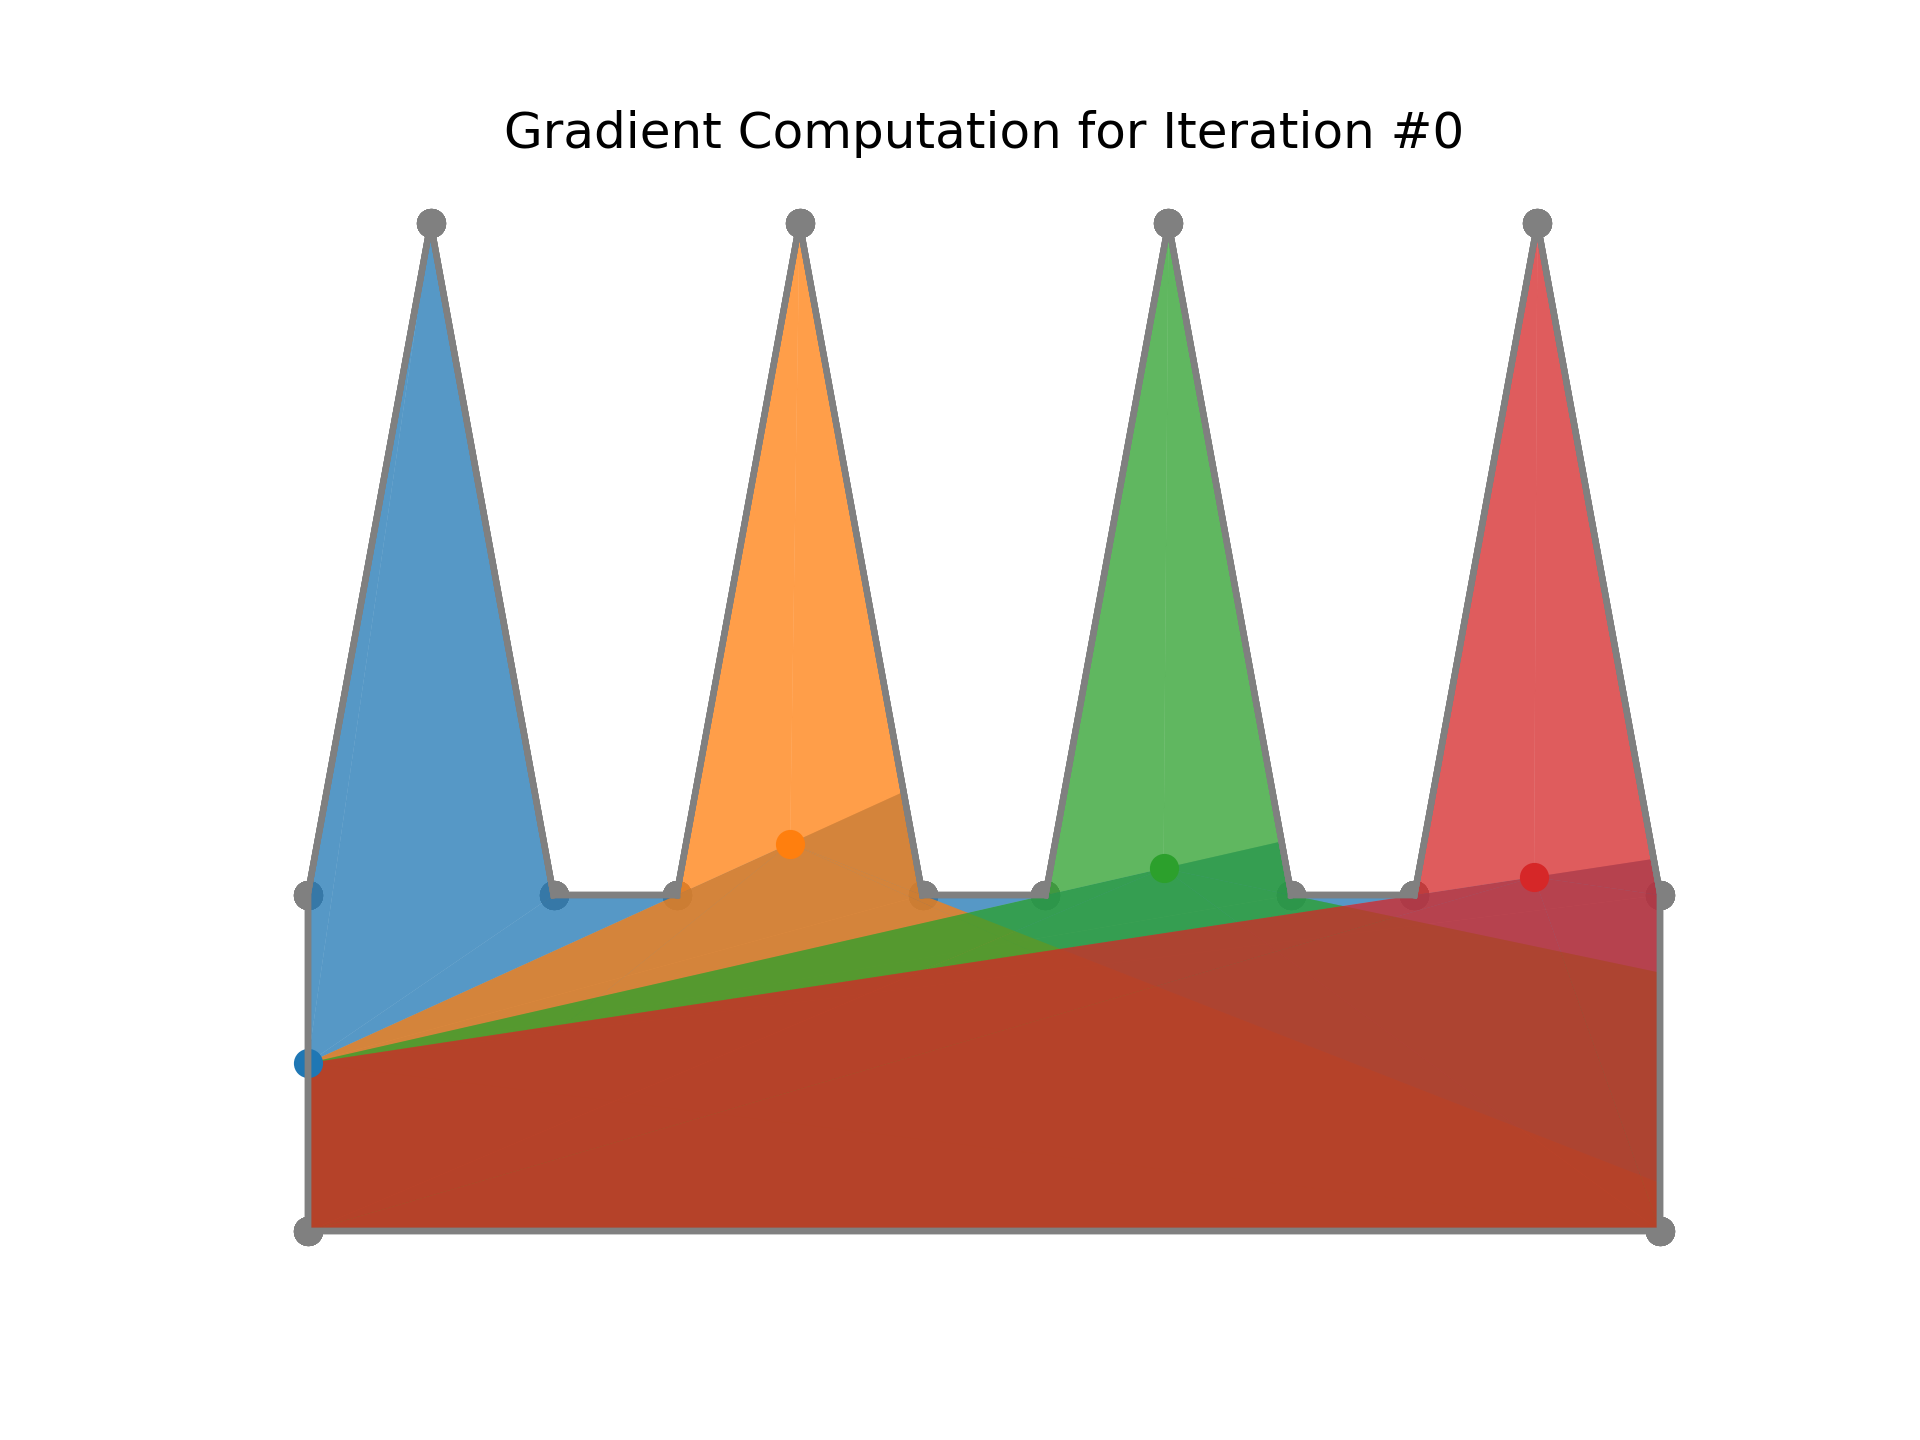
\includegraphics[width = 0.7\textwidth]{experiments/comb_greedy.png}
    \caption{The comb polygon with four teeth is already completely seen at greedy initialisation time.}
    \label{fig:comb_greedy}
\end{figure}

In the case of polygons who are not completely seen at initialisation time, it is unclear whether the greedy placement improves the overall progress. How well the algorithm behaves is highly dependent on the initial placement of the guards. Namely, the algorithm often does not finish with different starting positions (it is stuck in local optima). Because of this drawback, we cannot create extensive experiments with different starting guard positionings. It is additionally not feasible to find a generalisation in the type of placements that allow the algorithm to finish.

Therefore, we believe a randomised placement of the guards during the greedy initialisation would be beneficial for giving a head start to the algorithm. However, due to time constraints, this heuristic is to be explored more with a more robust algorithm implementation.
% - momentum
% - reflex vertex pull
    % - onto reflex vertex
    % - pull Capping
% - line search
% - reflex area
% - hidden gradient
% - angle behind reflex vertex
% - greedy initialisation

\subsection{Scaling for the Comb Polygon}
In this section we will observe how the algorithm scales on the comb polygon. We will take the comb polygons with 2, 3, ..., 10, 15, 20, 50, 100 teeth. We will note how the algorithm progresses in terms of the total area seen per iteration.
As such, we will run the algorithm with all heuristics for all the previously mentioned comb polygons. All guards will start at the same $y$-coordinate, 0.1 units apart from each other. An example of such a starting point can be found in Figure \ref{fig:comb6_start_pos}. In this way, we can ensure that the performance of the algorithm can be compared using the same starting position of the guards. We will deem a timeout of two hours for declaring an algorithm unfeasible for larger polygons. We will then analyse how the algorithm performed under each of the circumstances. Lastly, we will offer some points of improvement.

\begin{figure}[h!]
    \centering
    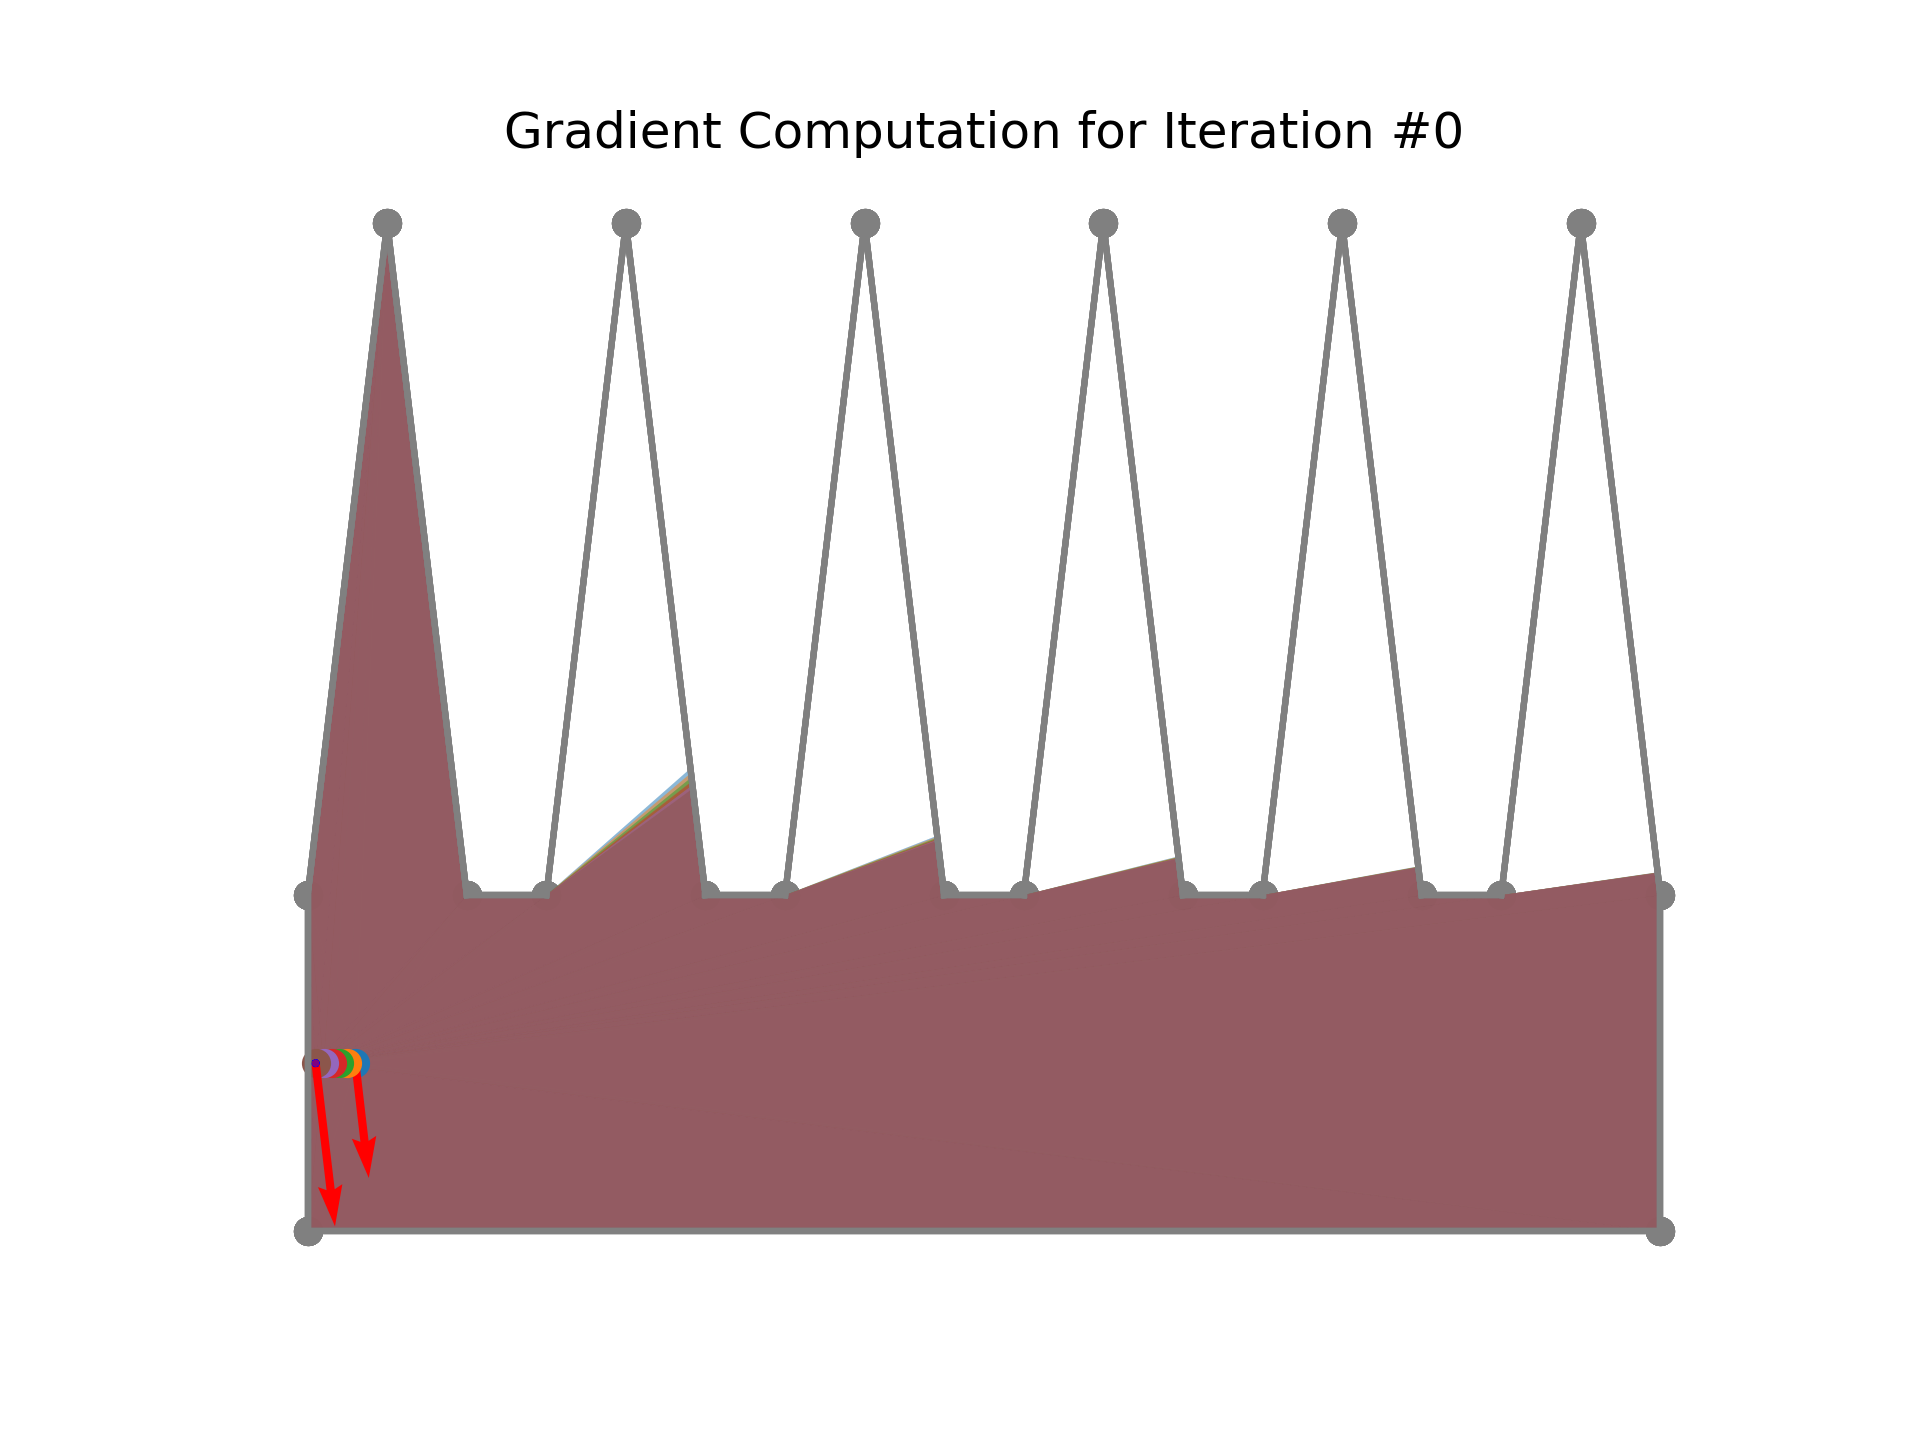
\includegraphics[width = 0.7\textwidth]{experiments/comb6_start_pos.png}
    \caption{In the comb polygon with 6 teeth, all guards start at the same $y$-coordinate, with 0.1 units in between them.}
    \label{fig:comb6_start_pos}
\end{figure}

We expect that the number of iterations needed would scale with the number of teeth of the polygon. We are also interested in how the execution time would scale. We expect that the time limit would already be achieved with less than 20 comb teeth.

Figure \ref{fig:all_combs} display the progression of our algorithm for the comb polygons with 2, 3, ..., 10, 15, 20 teeth within one hour. The comb polygons with 50 and 100 teeth did not complete any iteration within that time.
For comb polygons with 5 teeth and more than 6 teeth, the timeout was not enough to find a feasible solution. Nonetheless, it is worth discussing their behaviour, as it highlights the different issues the algorithm faces. 
For comb polygons with 7, 9 and 10 teeth, the guards appear to be stuck in a local plateau that it did not manage to escape. This can be traced to an edge case where the guards are stuck in their position because their movement vector does not improve the total area. Another reason why the guards do not move is that they are still trying to maximise their local viewed area in the case where the total area seen cannot be increased within that step. This could result in them all moving to the same part of the polygon. Since that part of the polygon maximises their locally seen area, they will not move anymore.
For comb polygon with 5 teeth, the guards appear to be stuck in a local maxima that they manage to escape. Unfortunately, they later return to it and restart the cycle. It is unclear whether the comb polygon with 8 teeth would display a similar looping behaviour. Given the timeout, the guards trying to solve the comb polygon with 8 teeth display a less predictable behaviour. We believe that hyperparameter tuning could address this issue.

\begin{figure}[h!]
    \centering
    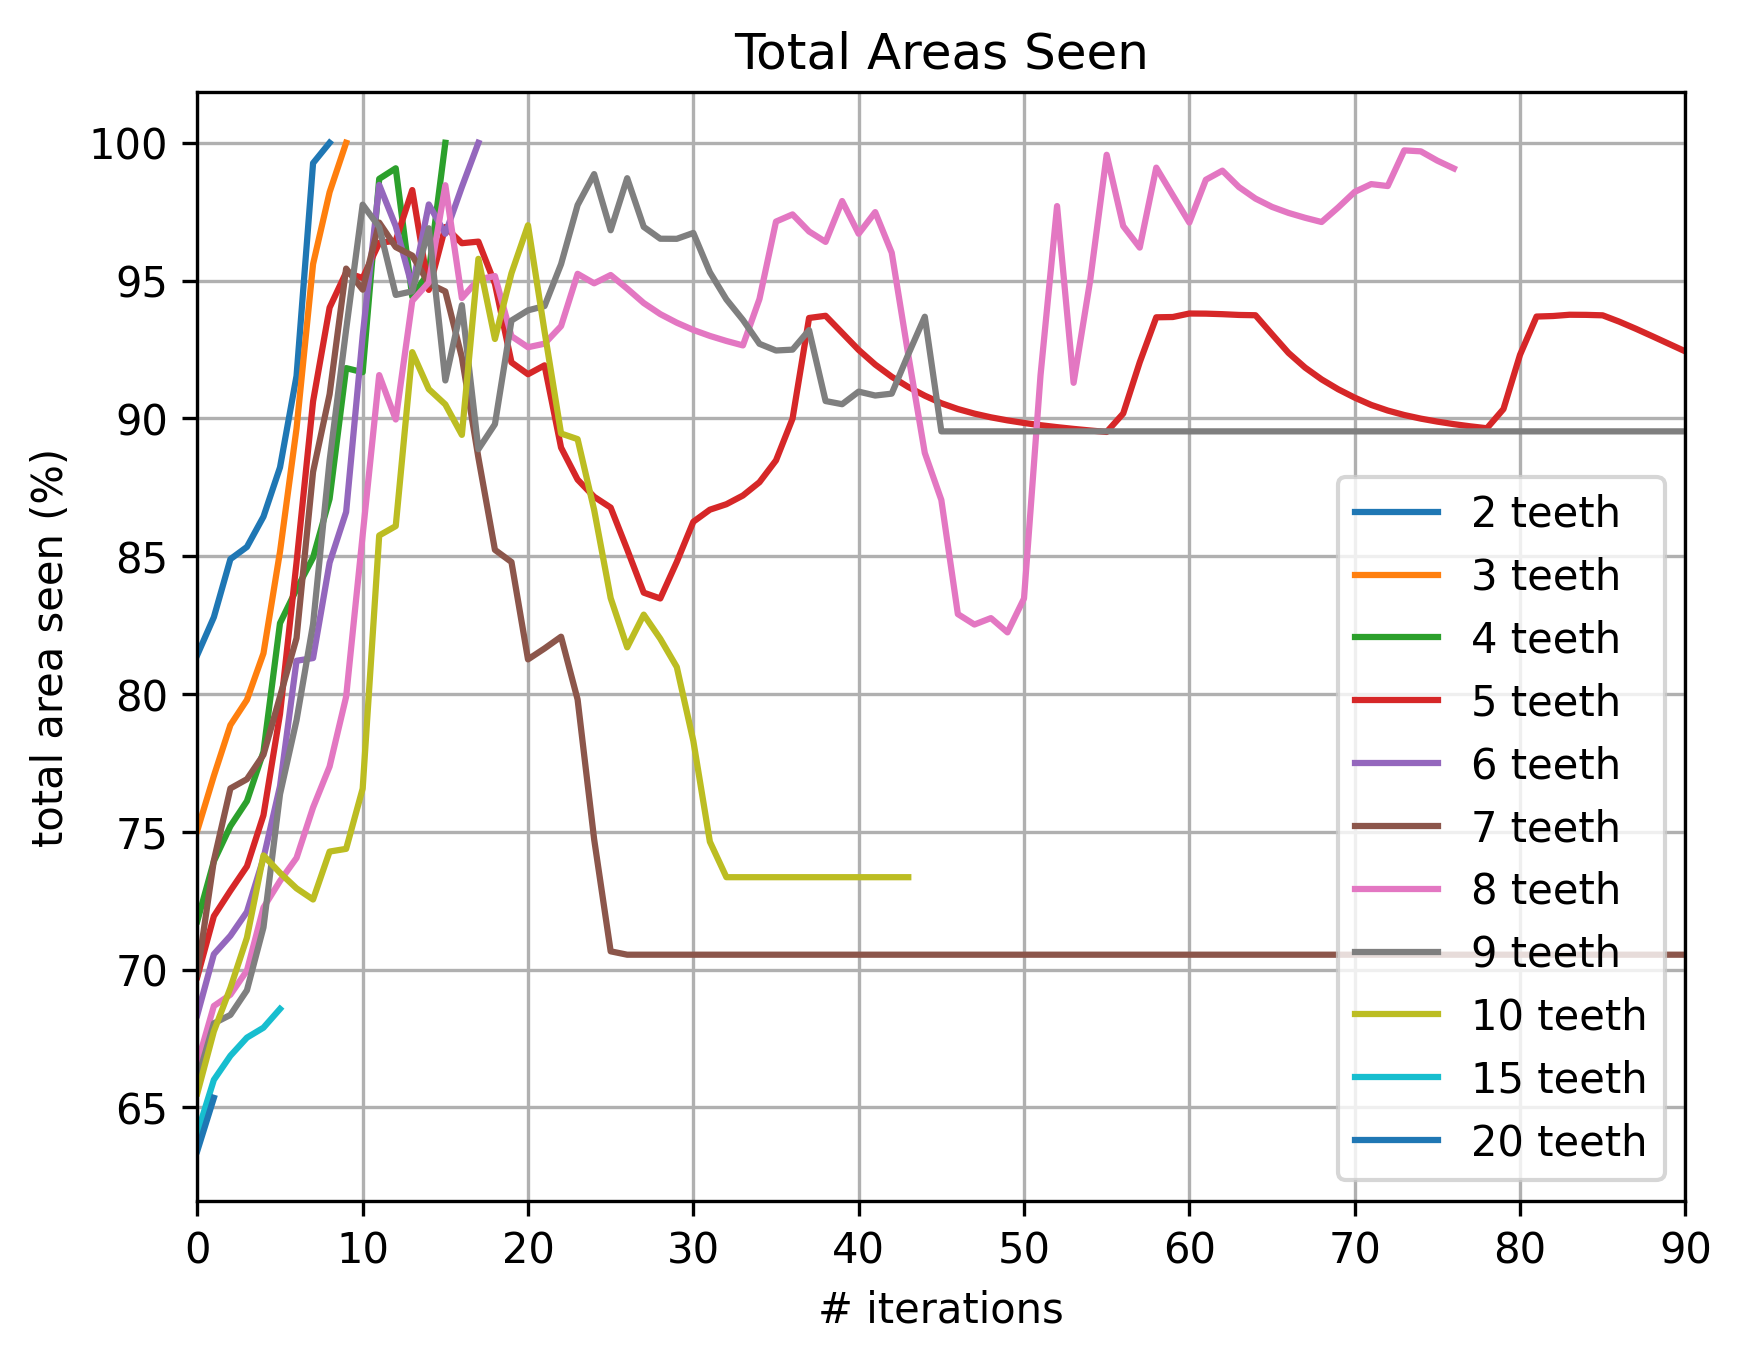
\includegraphics[width = \textwidth]{experiments/all_combs_areas.png}
    \caption{The percentage of the area seen in terms of iterations for comb polygons with 2, 3, ..., 10, 15, and 20 teeth.}
    \label{fig:all_combs}
\end{figure}

Conversely, it is also crucial to address the comb polygons which the algorithm manage to solve: 2, 3, 4 and 6 teeth. In this case, we can observe a clear scaling: the more teeth a comb polygon has, the longer it takes to be solved. What is more, the solution also scales with the number of teeth. The comb polygon with 4 and 6 teeth take twice as many iterations to be solved than the ones with 2 and 3 teeth, respectively. We would expect a similar behaviour for comb polygons with more teeth, if the algorithms would finish.

\begin{figure}[h!]
    \centering
    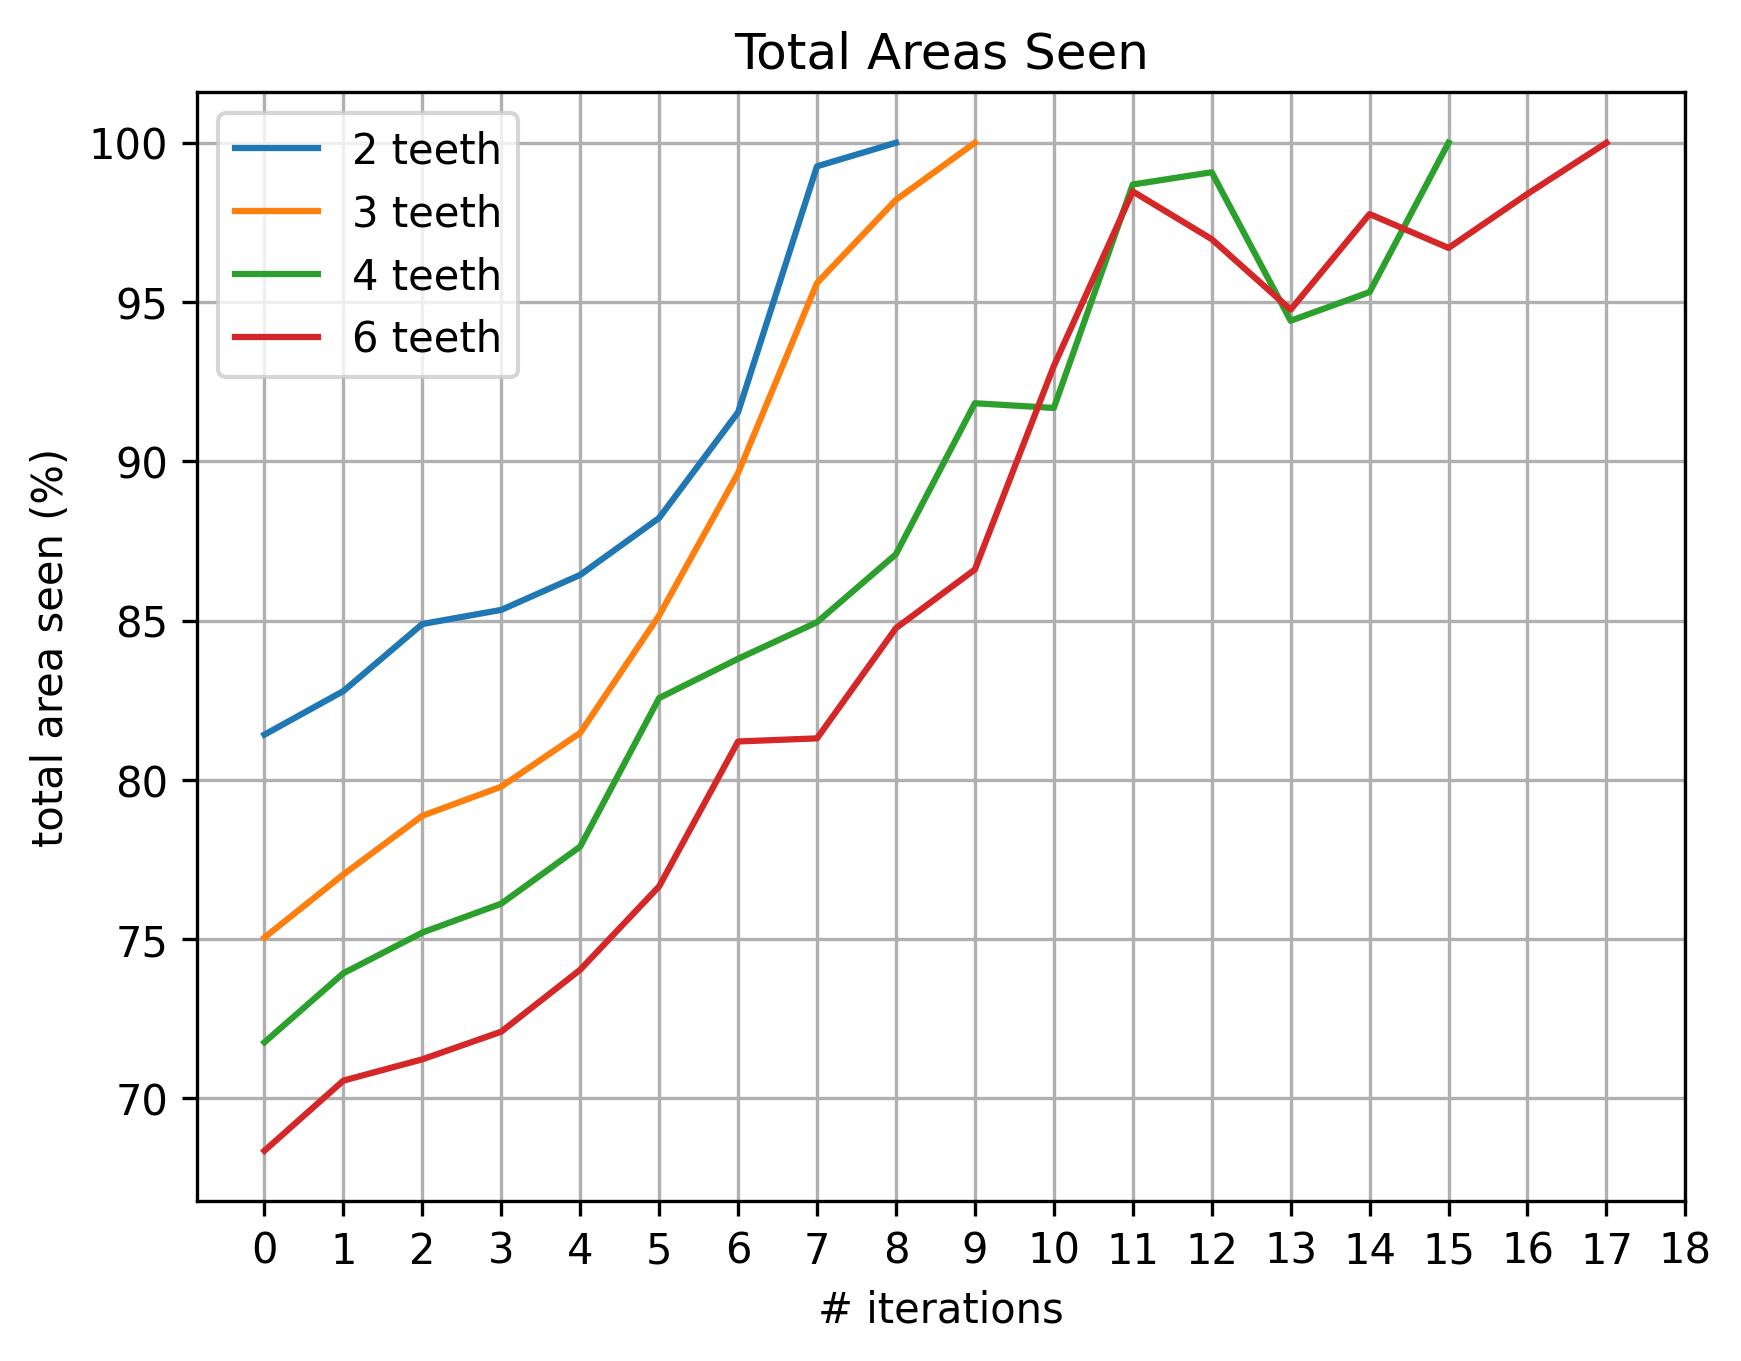
\includegraphics[width = \textwidth]{experiments/good_combs_areas.png}
    \caption{The percentage of the area seen in terms of iterations for comb polygons with 2, 3, 4, and 6 teeth.}
    \label{fig:good_combs}
\end{figure}

It is worth discussing how the initial guard placement and comb polygon shapes could influence the performance of the algorithm.
Firstly, it is importance to discuss the initial placement strategy. Guards are placed in the same lower left part of the polygon. However, the larger a polygon, the lower the initially seen area. For example, we can observe how the comb polygon with 2 teeth starts at more than 80\% seen area. On the other hand, the comb polygon with 20 teeth has a less than 65\% seen area at start. We could argue that this gives larger polygons a start disadvantage.
Moreover, the algorithm is sensitive to the shape of the polygons. The bigger a comb polygon grows, the sharper and narrower its teeth are. A good example in this case is Figure \ref{fig:comb20}, which displays a comb polygon with 20 teeth. Clearly, the teeth are much narrower than in the case of a comb with 4 teeth. This raises the question about the role the shape of the teeth plays into the algorithm performing better or worse. A possible solution to this aspect would be to scale up the polygon. However, a similar question would remain: does the algorithm necessarily perform better or worse because of the polygon shape? and what would be the optimal such shape?

\begin{figure}[h!]
    \centering
    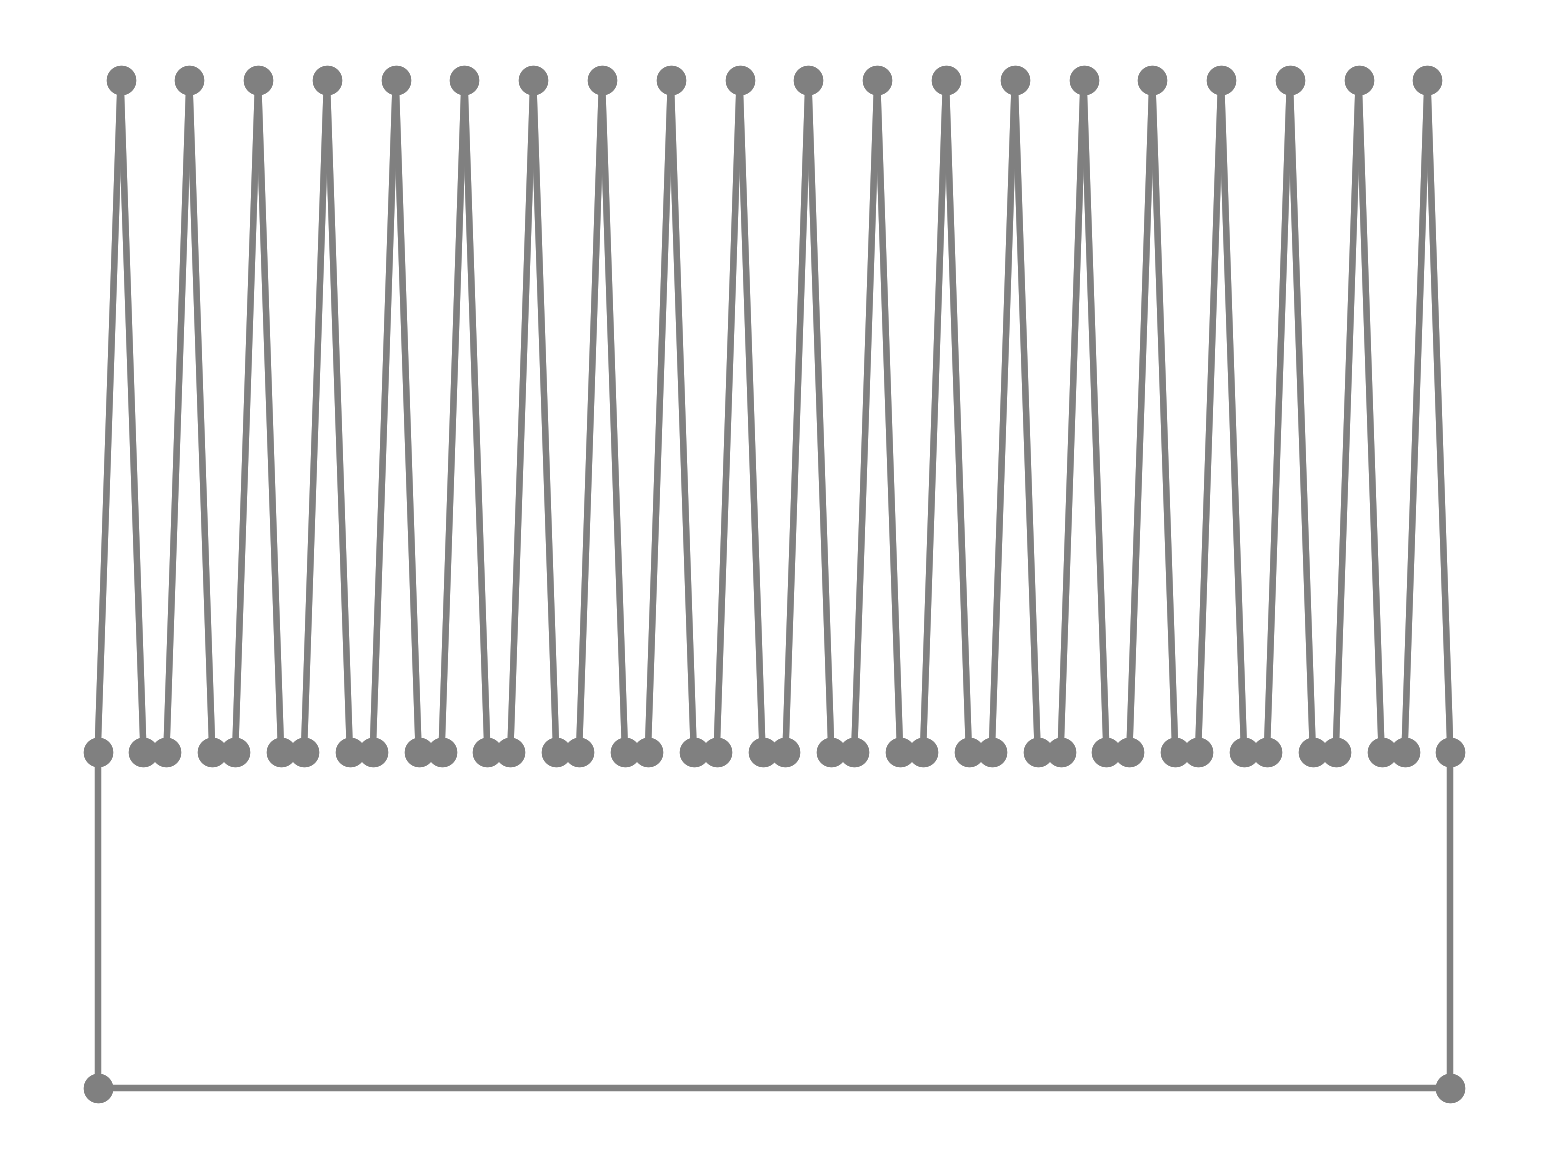
\includegraphics[width = 0.8\textwidth]{experiments/comb20.png}
    \caption{Comb polygon with 20 teeth.}
    \label{fig:comb20}
\end{figure}